\part{CÁLCULO INTEGRAL.}
\chapter{Integral Indefinida}
	
\section{Primitiva de una función}

Nuestro problema va a ser: dada $f:[a,b]\to \mathbb R$, ?`será posible encontrar otra función $F:]a,b[\to \mathbb R$, tal que su derivada coincida con $f$, es decir, que $F'(x)=f(x)\,$? Si es así, ?`será $F$ única?.

\begin{defi}
Sea $f:[a,b]\to \mathbb R$ una función real de variable real, decimos que 	$F:]a,b[\to \mathbb R$ es una \textbf{primitiva} de $f$ si y solo sí $F'(x)=f(x)$
\end{defi}

\begin{ejem}
$f(x)=2x \to F(x)=x^2$ es una primitiva de $f$, ya que $F'=2x=f$.

Pero $F(x)=x^2-5$ también lo es, y $F(x)=x^2+17 ; \; \cdots$

\end{ejem}

\begin{teor} 
Si una función $f(x)$ admite una primitiva $F(x)$, realmente tiene \textbf{infinitas primitivas}, todas las de la forma $F(x)+\mathcal C$	, siendo $\mathcal C$ una constante (un número real indeterminado). Esta $\mathcal C \in \mathbb R$ es la llamada \textbf{constante de integración.}
\end{teor}
\begin{proof}
Evidentemente: $ \left( F(x)+\mathcal C  \right)'=F'(x)+0=F'(x)=f(x)$
\end{proof}

\begin{ejem}
	Encontrar todas las primitivas de $f(x)=\cos x$
	
	$F(x)=\sin x + \mathcal C \textcolor{gris}{\quad \to \quad F'(x)=\cos x = f(x)}$
\end{ejem}

\section{Integral Indefinida}

\begin{defi}
Al conjunto de todas las primitivas de una función $f(x)$, es decir, a $F(x)+\mathcal C	$, se le llama \textbf{integral indefinida} de $f(x)$ y se denota así:

\begin{equation}
 \int f(x)\; \dd x = F(x) + \mathcal C	
\end{equation}

Expresión que se lee como `integral indefinida de $f(x)$ diferencial de $x$ es igual a $F(x)$ más la constante de integración' 

\end{defi}

\begin{ejem}
 Encuentra las siguientes integrales indefinidas.
\begin{multicols}{2}
$\displaystyle \int (2x)\; \dd x = x^2 + \mathcal C$	

$\displaystyle \int \cos x\; \dd x = \sin x + \mathcal C$
\end{multicols}	
\end{ejem}

La integración es la operación contraria a la derivación, incluso hay autores que a la primitiva (o a la integral indefinida) le llaman la \emph{antiderivada}.

	\begin{figure}[H]
			\centering
			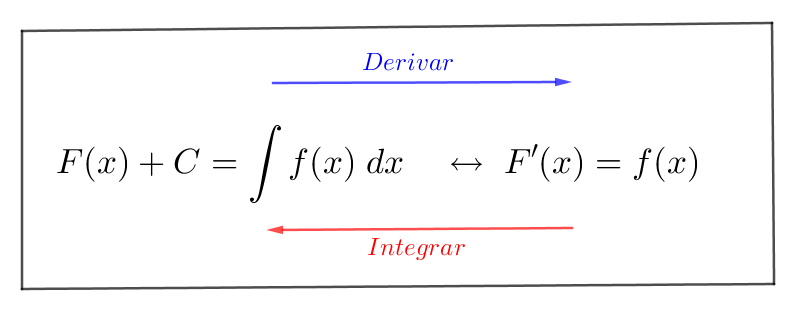
\includegraphics[width=0.7
			\textwidth]{imagenes/imagenes07/T07IM01.png}
		\end{figure}

	\begin{ejem}
		$F(x)=x^3+2x+3$, ?`es una primitiva de $f(x)=3x^2+2?$
		
	$F'(x)=(x^3+2x+3)'=	3x^2+2=f(x)\; $. Sí lo es, aunque sabemos que hay infinitas, esta es una de ellas.
	\end{ejem}

	\begin{ejem}
		Encuentra una primitiva $F(x)$ de $f(x)=3x^2+2$, tal que $F(-1)=2$
		
		En el ejemplo anterior hemos visto que una primitiva de $f(x)$ es  $F(x)=x^3+2x+3$, pero todas ellas son: $\displaystyle \int (3x^2+2) \; \dd x =x^3+2x+\mathcal C \to F(x) =x^3+2x+\mathcal C$
		
		Ahora vamos a determinar $\mathcal C$, pues tenemos que la primitiva $F(x)$ que buscamos ha de cumplir la condición $F(-1)=2$.
		
		$F(x)=x^3+2x+\mathcal C \to F(-1)=(-1)^3+2(-1)+\mathcal C= -3 + \mathcal C =2 \to \mathcal C=5  $
		
		La primitiva buscada es: $F(x)=x^3+2x+5$	
	\end{ejem}
	
	\section{Propiedades de las integrales indefinidas}
	
	\begin{teor}
	Si $F$ y $G$ son, respectivamente, primitivas de $f$ y $g$, entonces ($\to $), $F\pm G$ es una primitiva de $f \pm g$	
	\end{teor}
	\begin{proof}
		En efecto: $(F \pm G)'=F' \pm G'=f \pm g=(f\pm g)$, de donde:
		\begin{equation}
			\int (f(x)\pm g(x))\; \dd x = \int f(x)\; \dd x \pm \int g(x)\; \dd x 
		\end{equation}
	\centerline {\textbf{`La integral de la suma (resta) es la suma (resta) de integrales'.}	}
	\end{proof}
	
	\begin{teor}
	Si $F$ es una primitiva de $f$ y $ k\in \mathbb R$, entonces ($\to$), $k\cdot F$ es una primitiva de $k\cdot f$
	\end{teor}
	\begin{proof}
		Efectivamente, $(k\cdot F(x))'=k\cdot F'(x)=k\cdot f(x)=(k\cdot f(x))$, de donde
		\begin{equation}
			\int (k\cdot f(x))\; \dd x= k\cdot \int f(x)\; \dd x
		\end{equation}
		\centerline {\textbf{`En la integral de una constante por una función,}}
		\centerline {\textbf{podemos sacar la constante fuera del signo integral'}}
	\end{proof}
	\begin{teor} {LINEALIDAD DE LA INTEGRAL INDEFINIDA.}
	\label{linealidad-II}
		\begin{equation}
			\boxed{	\quad \int \left( a\; f(x)+ b\; g(x) \right) \; \dd x = a\cdot \int f(x) \; \dd x + b\cdot \int g(x) \; \dd x 	\quad}\; \; ; \quad a,b\in\mathbb R 
		\end{equation}
	\end{teor}
	
	\begin{ejem} Sabiendo que $\int e^x \dd x =e^x + \mathcal C_1 \quad \wedge \quad \int \cos x \dd x=\sin x + \mathcal C_2$, 
	
	calcula:  $\int (3e^x-2\cos x) \dd x$ 
	
	
	Por la linealidad de la integral indefinida, tenemos:
		
	$\int (3e^x-2\cos x) \; \dd x = 3 \cdot \int e^x \; \dd x - 2 \cdot  \int \cos x \; \dd x = 3\; e^x -2 \;  \sin x + \mathcal C$ 
	\end{ejem}
	
	\begin{teor} Integrales de las funciones elementales.	
	\begin{itemize}
		\item Funciones potenciales: Es evidente que $\int 5x^4\; \dd x= x^5 + \mathcal C \to \int x^4\; \dd x = \dfrac {x^5}{5} + \mathcal C$, de donde se deduce, en general: 
		
		$ \quad \boxed{  \int x^n \; \dd x = \dfrac {x^{n+1}}{n+1} + \mathcal C \; ; \; n\neq -1 } $
		
		\item Funciones logarítmicas ($n=-1$) :  $ \boxed{ \displaystyle  \int \dfrac 1 x \; \dd x = \mathrm{ln} \;  |x| + \mathcal {C} } $ , ya que $(\mathrm{ln} x)'=\dfrac 1 x$
		
		\item Funciones exponenciales: Como $(e^x)'=e^x$, deducimos: $\boxed{ \int e^x \; \dd x = e^x + \mathcal C }$
		
		\item Funciones trigonométricas Sabido que $(\sin x)'=\cos x$ y que $(\cos x)'=-\sin x$, tenemos: $\boxed{ \int \sin x \; \dd x= - \cos x + \mathcal C } \quad$ y $\quad \boxed{ \int \cos x \; \dd x=  \sin x + \mathcal C } $
		\item Trigonométricas inversas: Recordando las derivadas de $\arcsin x$ y de $arctan x$, podemos deducir: $\boxed{\displaystyle  \int \dfrac {1}{\sqrt{1-x^2}} \; \dd x = \arcsin x + \mathcal C } \quad $ y que $\quad \boxed{\displaystyle  \int \dfrac {1}{1+x^2} \; \dd x = \arctan x + \mathcal C } $
	\end{itemize}
	\end{teor}
	\begin{proof}
		Las demostraciones están incluidas en el propio teorema.
	\end{proof}

\begin{ejem}
Calcula $\int (5x^4-6x^3+4x-7) \; \dd x$	

Aplicando la linealidad de la integral indefinida, llamado por algunos autores `método de descomposición' para el cálculo integral y fijándonos en la integración de funciones potenciales que aparece en la tabla: $\displaystyle \int x^n \; \dd x = \dfrac {x^{n+1}}{n+1} +\mathcal{C}; \; n\neq -1$, tendremos:
	
	$\int (5x^4-6x^3+4x-7) \; \dd x= 5 \dfrac {x^5}{5}-6 \dfrac {x^4}{4} + 4 \dfrac {x^2}{2} -7x + +\mathcal{C} =	 x^5-3 \dfrac {x^4}{2} + 2 x^2 -7x + +\mathcal{C} $

\end{ejem}	

\begin{ejem} Calcula las siguientes integrales: 
\begin{multicols}{2}
\begin{enumerate}[a) ]
\item $\displaystyle \int \sqrt{x}\; \dd x$
\item $\displaystyle \int \dfrac {3 \sqrt[4]{x}}{5 \sqrt[3]{x^2}}\; \dd x$
\item $\displaystyle \int \left(4x^3-3x^2+2-\dfrac 5 x +\dfrac {7}{x^5} +\sin x  \right)\; \dd x $
\item $\displaystyle \int \tan^2 x \; \dd x $
\end{enumerate}
\end{multicols}
$\circ \quad a)\; $ Como $\sqrt{x}=x^{1/2}$, aplicamos la integral potencial y tenemos:

$\displaystyle \int \sqrt{x}\; \dd x =\displaystyle \int x^{1/2}\; \dd x = \dfrac {x^{1/2+1}}{1/2\; + \; 1}+ \mathcal C=\dfrac {x^{3/2}}{3/2\; + \; 1}+ \mathcal C=\dfrac { 2x \sqrt{x} } { 3 } + \mathcal C$

$\circ \quad b)\; $ Expresaremos el integrando como una única potencia e $x$ (división de potencias de la misma base) y usaremos la fórmula de integrales potenciales.

$\dfrac {3 \sqrt[4]{x}}{5 \sqrt[3]{x^2}}=\dfrac {3 \cdot  x^{1/4}}{5 \cdot x^{2/3}}= \dfrac 3 5 x^{1/4\; -\; 2/3}=\dfrac 3 5 x^{-5/3}$

$\displaystyle \int \dfrac {3 \sqrt[4]{x}}{5 \sqrt[3]{x^2}}\; \dd x=\displaystyle \int \dfrac 3 5 x^{-5/3} \; \dd x \; $ =[ linealildad de la I.I.] $\; = \displaystyle \dfrac 3 5 \int  x^{-5/3} \; \dd x = \dfrac 3 5 \cdot \dfrac {x^{-5/3+1}}{-5/3+1}+\mathcal C= \frac 3 5 \; \dfrac {x^{-2/3}}{-2/3}+ \mathcal c = \dfrac {-27}{10 \sqrt[3]{x^2}}+\mathcal C $

$\circ \quad c)\; $ Usando el método de descomposición (linealidad de la integral indefinida), podemos integrar directamente la integral como:

 $\displaystyle \int \left(4x^3-3x^2+2-\dfrac 5 x +\dfrac {7}{x^5} +\sin x  \right)\; \dd x = 4 \dfrac {x^4}{4}-3\dfrac {x^3}{3}-2 x-5 \mathrm{ln} |x|+ 7 \dfrac {x^-4}{-4}-\cos x + \mathcal C= x^4-x^3-2x-5 \mathrm{ln} |x|-\dfrac {7}{4x^4}-\cos x+\mathcal C$
 
 $\circ \quad d)\; $ Para esta integral vamos a necesitar `mucha ASTUCIA': sumaremos y restaremos $1$ al integrando (con lo cual, queda inalterado) y aplicaremos el método de descomposición. Conviene recordar  una de las formas de escribir $(\tan x)'=1+\tan^2 x$. Hay que reconocer que la primera vez que se ve esta forma de integrar $\tan^2 x$ asombra, pero con la práctica se le irán ocurriendo `ideas felices' también al lector.
 
 $\displaystyle \int \tan^2 x \; \dd x =\displaystyle \int (\tan^2 x  \; + 1 - \; 1)\; \dd x =\displaystyle \int (\tan^2 x \; + \; 1) \; \dd x - \displaystyle \int 1 \; \dd x = \tan x \; - x \; +\mathcal C$
\end{ejem}

\begin{teor} Integrales de las funciones compuesta ampliación de las fórmulas de integración obtenidas a la regla de la cadena.
	
	Funciones potenciales:  ahora, para poder tener como resultado de una integral de tipo potencial $\dfrac {f^{n+1} (x)}{n+1}$, en el integrando debe estar su derivada: 
	
	$\left( \dfrac {f^{n+1} (x)}{n+1} \right)' = \dfrac {1}{n+1} (n+1)\;  f^n (x)\cdot \textbf{f'(x)}$. Obsérvese que en el integrando debe aparecer, necesariamente, $\textbf{f'(x)}$, por ello: $   \int f^n \cdot \textbf{f'} \; \dd x = \dfrac {f^{n+1}}{n+1} + \mathcal C \; ; \; n\neq -1  $
		
		Y lo mismo ocurre para todas las integrales de las funciones elementales vistas anteriormente, p.e. como $(\cos f(x))'=- \textbf{f'(x)} \cdot \sin f(x)$.
		
		Las fórmulas anteriores se convierten en:
	
	\begin{multicols}{2}
			
	 $ \boxed{ \displaystyle \int f^n \cdot \textbf{f'} \; \dd x = \dfrac {f^{n+1}}{n+1} + \mathcal C \; ; \; n\neq -1 } $
	
	 $ \boxed{ \displaystyle  \int \dfrac 1 f \cdot \textbf{f'} \; \dd x = \mathrm{ln} \;  |f| + \mathcal {C} }$
	
	  $ \boxed{ \displaystyle \int e^f \cdot \textbf{f'} \; \dd x = e^f + \mathcal C } $
	
	 $ \boxed{ \displaystyle \int \textbf{f'} \cdot \sin f \; \dd x=  - \cos f + \mathcal C } $ 
	
	 $ \boxed{ \displaystyle \int \textbf{f'} \cdot \cos f \; \dd x=  \sin f + \mathcal C }  $
	

	  $ \boxed{ \displaystyle  \int \dfrac {\textbf{f'}} {\sqrt{1-f^2}} \; \dd x = \arcsin f + \mathcal C } $

	 $\boxed{ \displaystyle  \int \dfrac {\textbf{f'}}{1+f^2} \; \dd x = \arctan f + \mathcal C } $
	 
	 \end{multicols}

	 
	 \begin{figure}[H]
		\centering
		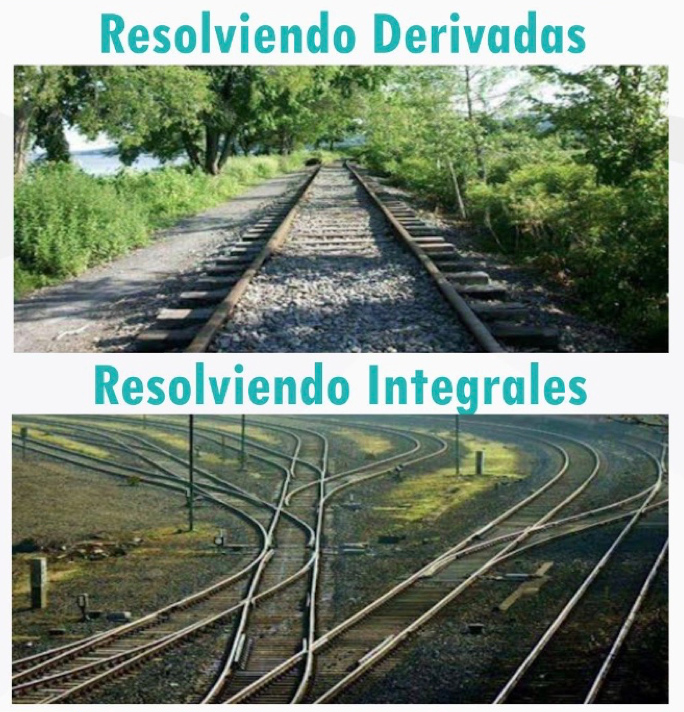
\includegraphics[width=0.5
		\textwidth]{imagenes/imagenes07/xiste07.png}
	\end{figure}

	
	
\end{teor}

\begin{proof}
	Las demostraciones están incluidas en el propio teorema.
\end{proof}

\begin{ejem} Integra las siguientes funciones:
\begin{multicols}{2}
\begin{enumerate}[a) ]
	\item $\displaystyle  \int (3x-2)^4\; \dd x$
	\item $\displaystyle  \int e^{5x} \; \dd x$
	\item $\displaystyle  \int \tan x \; \dd x$
	\item $\displaystyle  \int 5x^2  \; \cos (6x^3-5)\; \dd x$
\end{enumerate}
\end{multicols}

$\circ \quad a) \quad \displaystyle \int (3x-2)^4\; \dd x =\;$ \small{[necesitamos un 3 en el integrando : multiplicamos y dividimos por 3 y usamos la linealidad de la I.I.] }$\; = {\frac 1 3} \displaystyle \int 3 \; (3x-2)^4\; \dd x \; $ =[podemos aplicar la fórmula de integración potencial para funciones compuestas] = $\; \frac 1 3 \dfrac {(3x-4)^5}{5}+\mathcal C=  \dfrac {(3x-4)^5}{15}+ \mathcal C$

$\circ \quad b) \quad \displaystyle  \int e^{5x} \; \dd x= \displaystyle  \frac 1 5 \; \displaystyle \int 5 \; e^{5x} \; \dd x= \frac 1 5 e^{5x} + \mathcal C$

$\circ \quad c) \quad \displaystyle  \int \tan x \; \dd x = \displaystyle  \int \dfrac {\sin x}{\cos x} \; \dd x = $
$\displaystyle - \int (-sin x) \cdot \dfrac {1}{\cos x} \; \dd x $
$\textcolor{gris}{ = \displaystyle  \int \dfrac 1 f \cdot \textbf{f'} \; \dd x = \mathrm{ln} \;  |f| + \mathcal {C}} =$

$=- \mathrm{ln} |\cos x| + \mathcal C$

$\circ \quad d) \quad \displaystyle  \int 5x^2  \; \cos (6x^3-5)\; \dd x= $ 
\small{[ necesitamos un $18x^2$ dentro del símbolo integral, tenemos $5x^2$. No hay problema: el 5 puede salir y multiplicamos y dividimos por 18. !`Lo que no se pede hacer es multiplicar o dividir por $x$, solo por $k\in \mathbb R$! ]} 
$\; = \displaystyle 5 \int x^2  \; \cos (6x^3-5)\; \dd x =$

$= \displaystyle 5\; \frac 1 {18} \int 18 x^2  \; \cos (6x^3-5)\; \dd x \; $ = [ Usando la integración trigonométrica para funciones compuestas ] = $\; \frac 5 {18}\; \sin (6x^3-5)+ \mathcal C$ 

\end{ejem}
	

	
	\section{Tabla de integrales inmediatas}
	
	Se llaman así porque se obtienen directamente de las tablas de derivadas. 
	
	En el apéndice \ref{app:tabla-integrales} `Tabla de integrales inmediatas', aparecen más ampliada que aquí.
	

\begin{table}[h]
\centering
\def\arraystretch{2}
\begin{tabular}{|c|c|}
\hline
\multicolumn{2}{|c|}{Tabla de integrales inmediatas} \\ \hline
      \emph{Función elemental} & 	\emph{Función compuesta}      \\ \hline
  $\displaystyle \int k \; \dd x=kx+\mathcal{C}$    &  $\quad$        \\ \hline
   $\displaystyle \int x^n \; \dd x = \dfrac {x^{n+1}}{n+1} +\mathcal{C}; \; n\neq -1$         &   $\displaystyle \int f'\cdot  f^n \; \dd x = \dfrac {f^{n+1}}{n+1} +\mathcal{C}; \; n\neq -1$          \\ \hline
     $\displaystyle \displaystyle \int {\dfrac 1 x \; \dd x} = \mathrm{ln}|x|+\mathcal{C}$      &     $\displaystyle \displaystyle \int {\dfrac {f'} {f} \; \dd x} = \mathrm{ln}|f|+\mathcal{C}$       \\ \hline
 $\displaystyle \int e^x\; \dd x= e^x +\mathcal{C}$          &    $\displaystyle \int f' \cdot  e^f\; \dd x= e^f +\mathcal{C}$         \\ \hline
  $\displaystyle \int a^x\; \dd x= \dfrac {a^x}{\mathrm{ln}a} +\mathcal{C}$          &    $\displaystyle \int f' \cdot  a^f\; \dd x= \dfrac{a^f}{\mathrm{ln}a} +\mathcal{C}$         \\ \hline
  $\displaystyle \int \sin x \; \dd x= - \cos x + \mathcal{C}$         &  $\displaystyle \int f'\cdot \sin f \; \dd x= - \cos f + \mathcal{C}$           \\ \hline
    $\displaystyle \int \cos x \; \dd x=\sin x + \mathcal{C}$         &  $\displaystyle \int f'\cdot \cos f \; \dd x= \sin f + \mathcal{C}$           \\ \hline
     $\displaystyle \int \sinh x \; \dd x=  \cosh x + \mathcal{C}$         &  $\displaystyle \int f'\cdot \sinh f \; \dd x= \cosh f + \mathcal{C}$           \\ \hline
        $\displaystyle \int \cosh x \; \dd x=  \sinh x + \mathcal{C}$         &  $\displaystyle \int f'\cdot \cosh f \; \dd x= \sinh f + \mathcal{C}$           \\ \hline
    $\displaystyle \int \dfrac {1}{\sqrt{1-x^2}}\; \dd x = \arcsin x + \mathcal{C}$       &      $\displaystyle \int  \cdot \dfrac {f'}{\sqrt{1-f^2}}\; \dd x = \arcsin f + \mathcal{C}$         \\ \hline
     $\displaystyle \int \dfrac {1}{1+x^2}\; \dd x = \arctan x + \mathcal{C}$      &     $\displaystyle \int \dfrac {f'}{1+f^2}\; \dd x = \arctan f + \mathcal{C}$        \\ \hline
\end{tabular}
\end{table}

\section{Ejercicios de integrales inmediata.}
\subsection{Ejercicios resueltos de integrales inmediatas}

\begin{ejre} Calcula las siguientes integrales inmediatas:
\begin{multicols}{2}
\begin{enumerate}[a) ]
	\item $\displaystyle \int \dfrac {x^2-x+5}{x} \dd x$
	\item $\displaystyle \int (3x^2-5x+7-3\sqrt[4]{x^3}) \dd x$
	\item $\displaystyle \int \dfrac {6x^2-3}{4x^3-6x} \dd x$
	\item $\displaystyle \int \dfrac {1 + \tan^2 \sqrt{x}}{\sqrt{x}} \dd x$
	\item $\displaystyle \int \dfrac {\dd x}{\sqrt{3-5x^2}}$
	\item $\displaystyle \int \dfrac {3\; \dd x}{x\; \mathrm{ln} x}$
\end{enumerate}	
\end{multicols}
\end{ejre}

\begin{proofw}\renewcommand{\qedsymbol}{$\diamond$}	
Nos preguntaremos si nuestra integral es de tipo potencial o logarítmico ($n=-1$), exponcencial, tipo seno o coseno o tipo arcotangente o arcoseno. 

	$\circ \quad  a) \quad \displaystyle \int \dfrac {x^2-x+5}{x} \dd x= \displaystyle \int \left( x - 1 + 5 \dfrac 1 x  \right) \dd x= \dfrac {x^2}{2} - x +5 \mathrm{ln} |x|+ \mathcal C$
	
	$\circ \quad b) \quad \displaystyle \int (3x^2-5x+7-3\sqrt[4]{x^3}) \dd x= \displaystyle \int  (3x^2-5x+7-3x^{3/4}) \dd x= 3 \dfrac {x^3}{3} - 5 \dfrac {x^2}{2} +7x - 3 \dfrac {x^{7/4}}{7/4}+\mathcal C= x^3 -\dfrac 5 2 x^2 +7x - \dfrac {12}{7} \sqrt[4]{x^7}+\mathcal C $
	
	$\circ  \quad c) \quad \displaystyle \int \dfrac {6x^2-3}{4x^3-6x} \dd x= \displaystyle \int \dfrac {3(2x^2-1)}{2(2x^3-3x)} \dd x= \displaystyle \dfrac 3 2 \int \dfrac {(2x^2-1)}{(2x^3-3x)} \dd x =\; $ 
	
	\small{Esta integral es de tipo logarítmico, luego en el numerador necesitamos la derivada del denominador que es $6x^2-3$ y no $2x^2-1$. Lo arreglamos multiplicando y dividiendo por $3$ (más fácilmente, introduciendo el $3$ que hemos sacado del numerador)} 
	
	$\; =\displaystyle \dfrac 3 2 \; \dfrac 1 {(3)} \int \dfrac {(3)\cdot (2x^2-1)}{(2x^3-3x)} \dd x= \displaystyle  \dfrac 1 2 \int \dfrac {6x^2-3}{(2x^3-3x)} \dd x= \dfrac 1 2 \mathrm{ln} |2x^3-3x| + \mathcal C$
	
	$\circ \quad d) \quad \displaystyle \int \dfrac {1 + \tan^2 \sqrt{x}}{\sqrt{x}} \dd x = \displaystyle \int  \dfrac {1} {\sqrt{x}} \cdot (1 + \tan^2 \sqrt{x}) \;  \dd x\; = $ 
	
	\small{ tenemos una integral de tipo $\tan x; \mbox{ ya que } (\tan x)'=1+\tan^2 x	$ ; solo nos falta la `regla de la cadena': $(\tan \sqrt(x))' = (1+\tan^2 \sqrt(x))\cdot (\sqrt(x))'$, pero $( \sqrt{x} )'=\dfrac {1}{2 \sqrt{x}}\; $ }
	
	$= \displaystyle 2 \int  \dfrac {1} {2\sqrt{x}} \cdot (1 + \tan^2 \sqrt{x}) \;  \dd x= 2 \tan \sqrt x + \mathcal C$ 
	
	$\circ \quad e) \quad \displaystyle \int \dfrac {\dd x}{\sqrt{3-5x^2}}=\;$ [Esta integral `tiene pinta' de $\arcsin f$]  $=\; \displaystyle \int \dfrac {\dd x}{\sqrt{3(1-\frac 5 3 x^2)}}= \dfrac {1}{\sqrt{3}} \displaystyle \int \dfrac {\dd x}{\sqrt{1-\frac 5 3 x^2}}= \dfrac {1}{\sqrt{3}} \displaystyle \int \dfrac {\dd x}{ \sqrt {1- \left( \frac {\sqrt 5} {\sqrt 3} x \right)^2} } = $ 
	
	 Para aplicar la regla de la cadena, falta tener en el integrando $f'=\left( \sqrt{\dfrac 5 3 }\; x \right)'=\sqrt{\dfrac 5 3}$;  pues multiplicamos y dividimos por $\sqrt{\dfrac 5 3}\; $ 
	
	$ = \dfrac {1}{\sqrt{3}}\cdot \dfrac {1}{\sqrt{\dfrac 5 3}} \displaystyle \int \dfrac {\sqrt{\dfrac 5 3}}{ \sqrt {1- \left( \frac {\sqrt 5} {\sqrt 3} x \right)^2} } \; \dd x = \dfrac {\sqrt{5}}{5	}\; \arcsin \left(\sqrt{\frac 5 3}\; x  \right) + \mathcal C$
	
	$\circ \quad f) \quad  \displaystyle \int \dfrac {3\; \dd x}{x\; \mathrm{ln} x} = \displaystyle 3 \int \dfrac {1 }{x}\; \dfrac {1}{\mathrm{ln} x} \; \dd x =\; $ [ Como  $(\mathrm{ln} x)'= 1/x$, tenemos una integral de tipo logarítmico:$\;\;$ ] $\;\; \; =\; 3\;  \mathrm {ln}\;  (\mathrm{ln} \;  x) + \mathcal C$
	
	\end{proofw}

\begin{ejre} Calcula las siguientes integrales inmediatas:
\begin{multicols}{2}
\begin{enumerate}[a) ]
	\item $\displaystyle \int \sqrt{x} (x^3+1) \dd x$ 
	\item $\displaystyle \int 3x (x^2+2)^3 \dd x$
	\item $\displaystyle \int \dfrac {(1+\sqrt x)^2}{\sqrt x} \dd x$
	\item $\displaystyle \int \dfrac {3x\dd x}{\sqrt[3]{x^2+3}}$
	\item $\displaystyle \int \sin^3 x \; \cos x \; \dd x$
	\item $\displaystyle \int \dfrac {e^x}{2e^x-3} \dd x$
\end{enumerate}	
\end{multicols}
\end{ejre}
	
\begin{proofw}\renewcommand{\qedsymbol}{$\diamond$}
	
Nos preguntaremos si nuestra integral es de tipo potencial o logarítmico ($n=-1$), exponcencial, tipo seno o coseno o tipo arcotangente o arcoseno. 

$\circ \quad  a) \quad \displaystyle \int \sqrt{x} (x^3+1) \dd x\; $ [ multipliquemos el integrando ] =$\; \displaystyle \int x^{1/2} (x^3+1) \dd x =\displaystyle \int  (x^{7/2}+x^{1/2}) \dd x= \dfrac {x^{9/2}}{9/2} + \dfrac {x^{3/2}}{3/2} + \mathcal C= \dfrac {2 \sqrt{x^2}}{9} + \dfrac {2 \sqrt{x^3}}{3} + \mathcal C$
	
$\circ \quad b) \quad \displaystyle \int 3x (x^2+2)^3 \dd x\; $ = [ la integral es de tipo potencial, arreglemos $f'$ ]=

$\; = \displaystyle 3  \frac 1 2 \int 2x (x^2+2)^3 \dd x= \frac 3 2 \dfrac {(x^2+3)^3}{3}+\mathcal C=\dfrac {(x^2+3)^3}{2}+\mathcal C$

$\circ \quad c) \quad \displaystyle \int \dfrac {(1+\sqrt x)^2}{\sqrt x} \dd x\; $ =[ Esta integral es de tipo potencial ] =
$\; \displaystyle (2) \int \dfrac {1} {(2)\sqrt{x}} \cdot  ( 1+\sqrt{x} )^2 \dd x = 2  \dfrac {( 1+\sqrt{x} )^3}{3}+\mathcal C=    \dfrac {2( 1+\sqrt{x} )^3}{3}+\mathcal C$

$\circ \quad d) \quad \displaystyle \int \dfrac {3x\dd x}{\sqrt[3]{x^2+3}}= 3 \displaystyle \int \dfrac {x\dd x}{\sqrt[3]{3(1/3\; x^2+1)}}=\dfrac {3} {\sqrt[3]{3}} \displaystyle \int \dfrac {x\dd x}{ \sqrt[3] {\left( \dfrac  {x^2}{3}+1 \right)}  }\;= $ 

Si $f=x^2/3 \to f'=2/3 \; x\;$, luego necesitamos $2/3$ en el numerador del integrando 
 
  $\; =  \dfrac {3} {\sqrt[3]{3}} \left( \dfrac 3 2 \right)  \displaystyle \int \dfrac {\left(\dfrac 2 3 \right)x\dd x}{ \sqrt[3] { \left( \dfrac  {x^2}{3}+1 \right) }  } = \dfrac {9}{2 \sqrt[3]{3} } \displaystyle \int \dfrac {2x}{3} \left(\dfrac {x^2}{3}+1  \right)^{1/3}\; \dd x= \dfrac {9}{2 \sqrt[3]{3} } \dfrac {\left(\dfrac {x^2}{3}+1  \right)^{1/3+1}}{1/3 + 1}+ \mathcal C= \dfrac {27}{8 \sqrt[3]{3} } \dfrac {\left(\dfrac {x^2}{3}+1  \right)^{1/3+1}}{4/3}+ \mathcal C=\dfrac {27}{ 8 \sqrt[3]{3} } \sqrt[3] { \left (\dfrac {x^2}{3} + 1  \right)^{4} } + \mathcal C $ 

$\circ \quad e) \quad \displaystyle \int \sin^3 x \; \cos x \; \dd x\; $ =[ Esta integral es claramente potencial ]= $\;  \dfrac {\sin^4 x}{4}+\mathcal C$

$\circ \quad f) \quad \displaystyle \int \dfrac {e^x}{2e^x-3} \dd x= \displaystyle \int e^x \; \dfrac {1}{2e^x-3} \dd x$ =\small{[ integral típicamente potencial, a falta de un 2 en el numerador, pero $n=-1$, logarítmica pues ]}=$ \; \dfrac {1}{(2)}\displaystyle \int (2) e^x \; \dfrac {1}{2e^x-3} \dd x= \dfrac {\mathrm{ln}|2e^x-3|}{2}+\mathcal C$ 
\end{proofw}

\begin{ejre} Calcula las siguientes integrales inmediatas:
\begin{multicols}{2}
\begin{enumerate}[a) ]
	\item $\displaystyle \int (1+\tan x)^2 \dd x$
	\item $\displaystyle \int \left( \dfrac {e^x-4}{e^{2x}}\right) \dd x$
	\item $ \displaystyle \int \frac {2 \sin x \; \cos x}{1+\sin^2 x} \dd x$
	\item $\displaystyle \int \frac {\cos x}{1+\sin^2 x} \dd x$
	\item $\displaystyle \int x\; e^{\sin (x^2)}\; \cos (x^2)\; \dd x$
	\item $\displaystyle \int \dfrac {\sin(\mathrm{ln}x)}{x} \dd x$
\end{enumerate}	
\end{multicols}
\end{ejre}
	
\begin{proofw}\renewcommand{\qedsymbol}{$\diamond$}	

	$\circ \quad a) \quad \displaystyle \int (1+\tan x)^2 \dd x = \displaystyle \int (1+2\tan x +\tan^2 x) \dd x= \displaystyle \int (1 +\tan^2 x) \dd x + \displaystyle \int 2\tan x  \dd x = \tan x - 2 \mathrm{ln}|\cos x|+ \mathcal C$


 	\hspace{-7mm} $\circ \quad b) \quad \displaystyle \int \left( \dfrac {e^x-4}{e^{2x}}\right) \dd x= \displaystyle \int (e^{-x} -4e^{-2x})   \dd x=\displaystyle (-1) \int (-1)\; e^{-x}    \dd x+\displaystyle -4  \dfrac {1}{(-2)} \int (-2)\; e^{-2x}    \dd x = -e^{-x} +2 e^{-2x}+\mathcal C$
	
 	\hspace{-7mm} $\circ \quad c) \quad \displaystyle \int \frac {2 \sin x \; \cos x}{1+\sin^2 x} \dd x= \displaystyle \int (2 \sin x \; \cos x)\cdot  \frac {1}{1+\sin^2 x} \dd x \; $ = \small{[ tipo logarítmico ]} \normalsize{=} $\;  \mathrm{ln} (1+\sin^2 x) +\mathcal C\; $ \small{( nótese que es este caso no hemos puesto $|\cdot|$ al logaritmo al ser su argumento siempre positivo )} \normalsize{.}
	
 	\hspace{-7mm} $\circ \quad d) \quad \displaystyle \int \frac {\cos x}{1+\sin^2 x} \dd x= \displaystyle \int \frac {\cos x}{1+(\sin x)^2} \dd x\; $ \small{ [ integral claramente de tipo arcotangente ] } \normalsize{$\; =  \arctan (\sin x) + \mathcal C$}
	
 	\hspace{-7mm} $\circ \quad e) \quad \displaystyle \int x\; e^{\sin (x^2)}\; \cos (x^2)\; \dd x= \displaystyle \dfrac {1}{(2)} \int (2) x\; \cos (x^2)\;  e^{\sin (x^2)} \; \dd x =\frac 1 2  e^{\sin^2 x}+ \mathcal C$
	
	   \hspace{-7mm} $\circ \quad f) \quad \displaystyle \int \dfrac {\sin(\mathrm{ln}x)}{x} \dd x = \displaystyle \int \dfrac 1 x \cdot \sin(\mathrm{ln}x) \dd x = - \cos(\mathrm{ln})x + \mathcal C$
\end{proofw}

\begin{ejre} Calcula las siguientes integrales inmediatas:
\begin{multicols}{2}
\begin{enumerate}[a) ]
	\item $\displaystyle \int \dfrac {\sen x - \cos x}{\sin x + \cos x} \; \dd x$
	\item $\displaystyle \int \sin x \; \cos x  \; \dd x$
	\item $\displaystyle \int \dfrac {x}{\sqrt{1-x^4}} \; \dd x$
	\item $\displaystyle \int \sin x \;  3^{\; \cos x + 2} \; \dd x$
	\item $\displaystyle \int \dfrac {1}{x\; \mathrm{ln}x} \; \dd x$
	\item $\displaystyle \int \dfrac {1}{\sqrt{x}(1+x)} \; \dd x$
\end{enumerate}	
\end{multicols}
\end{ejre}
	
\begin{proofw}\renewcommand{\qedsymbol}{$\diamond$}	



	$\circ \quad a) \quad \displaystyle \int \dfrac {\sen x - \cos x}{\sin x + \cos x} \; \dd x = \displaystyle (-1)\int \dfrac {-\sen x +\cos x}{\sin x + \cos x} \; \dd x = \displaystyle -1\int \dfrac {\cos x - \sin x}{\sin x + \cos x} \; \dd x = \; $ \small{ [ el numerador es directamente el denominador ] } = \normalsize{$ - \mathrm{ln} \left| \sin x + \cos x \right| + \mathcal C$}
	
	
	$\circ \quad b) \quad \displaystyle \int \sin x \; \cos x  \; \dd x= \;$  
	
Integral de tipo potencial, podemos considerar tanto $f=\sin x$ como $f=\cos x$, pero elegiremos la primera, ya que el $\cos x = f'$ directamente, sin necesidad de introducir ningún signo menos. Si elegimos la otra opción obtenemos otro resultado pero, al  diferir en una constante, se trata de la misma integral (relación fundamental de la trigonometría) 

$\;= \displaystyle \int (\sin x)^1 \; \cos x  \; \dd x = \dfrac {(\cos x)^2}{2} + \mathcal C  = \dfrac {\cos^2 x}{x} + \mathcal C$
	
	$\circ \quad c) \quad \displaystyle \int \dfrac {x}{\sqrt{1-x^4}} \; \dd x= \displaystyle  \dfrac{1}{(2)} \int \dfrac {(2)\; x}{\sqrt{1-(x^2)^2}} \; \dd x= \; $ \small{[ integral de tipo arcoseno ]} \normalsize{ $\; = \dfrac 1 2 \arcsin x + \mathcal C $}
	
	$\circ \quad d) \quad \displaystyle \int \sin x \; 3^{\; \cos x + 2} \; \dd x= \; $ \small{[ integral de tipo exponencial, pero la base no es $e$, la diferencia es que ahora se arrastra una constante $\mathrm{ln}3$. Ver apéndice \ref{app:tabla-integrales} `Tabla de integrales inmediatas' ]} \normalsize{}$\; = \displaystyle(-1) \int -\sin x \; 3^{\; \cos x + 2} \; \dd x= - \dfrac {3^{\; \cos x + 2}}{\mathrm{ln}3} + \mathcal C$
	
	$\circ \quad e) \quad \displaystyle \int \dfrac {1}{x\; \mathrm{ln}x} \; \dd x= \int \dfrac {1}{x} \cdot \dfrac {1} {\mathrm{ln}x} \; \dd x =\; $ \small{[ Integral tipo logarítmico ]} \normalsize{ $\; = \mathrm {ln} |\mathrm {ln} x| + \mathcal C$}
	
	$\circ \quad f) \quad \displaystyle \int \dfrac {1}{\sqrt{x}(1+x)} \; \dd x = \; $ \small{[Esta integral, de tipo arcotangente, requiere de cierta astucia]}  \normalsize{$\; = \displaystyle (2) \int \dfrac {1}{(2) \sqrt{x} \left( 1+(\sqrt{x})^2 \right)} \; \dd x =(2) \int \dfrac {1}{(2) \sqrt{x}} \; \dfrac {1}{\ 1+(\sqrt{x})^2 } \; \dd x =2 \arctan (\sqrt{x})+\mathcal C$}
\end{proofw}

\begin{teor}{Integrales inmediatas de valores absolutos.}

Se trata de integrar funciones de la forma 

$F(x)= \int |f(x)| \dd x$ donde $F(x)$ es una primitiva cualquiera. 

Como $f(x)$ es ctna., tanbién lo es $|f(x)|$, por tratarse de una composición de funciones continuas.

Romperemos $f(x)$ a trozos e integraremos a trozos. Para cada trozo aparecerá una constante de integración $C_i$, que guardarán relación entre ellas, pues:

Al ser $F(x)$ derivable, necesariamente será continua (ver teorema y demostración \ref{teor:deriv-cont}). 

Al exigir que $F(x)$ sea continua, determinaremos las relaciones entre las distintas constantes de integración que aparecerán y quedará la primitiva en función de una sola constante de integración.
\end{teor}

\begin{proof}
Recordad el teorema de que derivabilidad implica continuidad, visto en el capitulo \ref{ch-la-derivada}, teorema \ref{teor:deriv-cont}

Como, evidentemente, $F(x)$ es derivable: $F'(x)=|f(x)|$	 (la derivada de la primitiva (o de la integral indefinida) es el integrando). Luego, necesariamente, $F(x)$ ha de ser continua.
\end{proof}


\begin{ejre} Calcula:
	
		 $a) \quad \displaystyle \int |x+2| \; \dd x \qquad$
		 $b) \quad \displaystyle \int (3+|x|) \; \dd x \qquad$
		 $c) \quad \displaystyle \int 3x\: |x-2| \; \dd x $
	
\end{ejre}
\begin{proofw}\renewcommand{\qedsymbol}{$\diamond$}


$a) \quad$ Rompamos la función $f(x)=\begin{cases}
								-x-2 &; \; x<-2 \\
								x+2  &; \; x\ge -2
								\end{cases}\; $ Y ahora, integremos a trozos.
	$F(x)=\begin{cases}
			-\frac {x^2}{2}-2x+\mathcal {C}_1 &; \; x<-2 \\
			\frac {x^2}{2}+2x+\mathcal {C}_2  &; \; x\ge -2
			\end{cases}\; $ Exijamos ahora que $F$ sea ctna. en $x=-2$.
			
	Vamos a aplicar el método rápido (recordad que, para mayor rigor, hay que seguir el método de los tres pasos (definición \ref{def-ctndad}).
	
	$F_-(2)=2+\mathcal {C}_1=F_+(-2)=6+\mathcal {C}_2 \to \mathcal {C}_2=4+\mathcal {C}_1$ Llamado $\mathcal {C}_1=\mathcal {K}$, podemos escribir $F(x)$ así:
	
	$F(x)=\begin{cases}
			-\frac {x^2}{2}-2x+ \mathcal {K} &; \; x<-2 \\
			\frac {x^2}{2}+2x+4+\mathcal {K}  &; \; x\ge -2
			\end{cases}\; $

$b) \quad$ Rompamos la función $f(x)=\begin{cases}
								3-x  &; \;  x<0 \\
								3+x  &; \;  x\ge 0
								\end{cases} \;$ 


Integramos a trozos: $F(x)=\begin{cases}
						-\frac {x^2}{2}+\mathcal{C}_1 &; \; x<0 \\
						\frac {x^2}{2}+\mathcal{C}_2 &; \; x\ge 0
								\end{cases}$
								
$F$ ha de ser ctna. en $x=0 \to F_-(0)=\mathcal {C}_1=F_+(0)=\mathcal {C}_2 \to \mathcal {C}_1=\mathcal {C}_2=\mathcal {K}$

Luego: $F(x)=\begin{cases}
			-\frac {x^2}{2}+\mathcal{K}&; \; x<0 \\
			\frac {x^2}{2}+\mathcal{K} &; \; x\ge 0
			\end{cases}$
			
$c) \quad$ Rompamos la función $f(x)=\begin{cases}
								-3x^2+6x+  &; \;  x<2 \\
								3x^2-6x  &; \;  x\ge 2
								\end{cases} \;$
							
Integramos a trozos: $F(x)=\begin{cases}
				-x^3+3x^2+\mathcal{C}_1 &; \; x<2 \\
				x^3-3x^2+\mathcal{C}_2 &; \; x\ge 2
					\end{cases}$
					
Exigimos ctndad. en $x=2 \to F_-(2)=4+\mathcal{C}_1=F_+(2)=-4+\mathcal{C}_2 \to \mathcal{C}_2=8+\mathcal{C}_1$, llamando $\mathcal{C}_1=\mathcal{K}; \; \; F(x)\; $ será:

 $F(x)=\begin{cases}
		-x^3+3x^2+\mathcal{K} &; \; x<2 \\
		x^3-3x^2+8+\mathcal{K} &; \; x\ge 2
		\end{cases}$


\end{proofw}

\subsection{Ejercicios propuestos de integrales inmediatas}
\begin{multicols}{2}
\begin{enumerate}[a) ]
\item $\displaystyle \int \dfrac {\sin x}{\sqrt{\cos x}} \dd x \textcolor{gris}{= -2 \sqrt{\cos x}+\mathcal C}$ 
\item $\displaystyle \int \dfrac {x^2}{x^3-2} \dd x \textcolor{gris}{=\dfrac 1 3 \mathrm{ln} |x^3-2|+\mathcal C}$
\item $\displaystyle \int \dfrac {e^{\tan x}}{\cos^2 x} \; \dd x \textcolor{gris}{= e^{\tan x} +\mathcal C}$ 
\item $\displaystyle \int \dfrac {1}{2+3x^2} \; \dd x \textcolor{gris}{ = \dfrac {\sqrt{6}}{6}\; \arctan \left( \sqrt{ \dfrac {3x}{2} } \right) +\mathcal C }$ 
\item $\displaystyle \int \dfrac {1}{(x-3)^2} \; \dd x \textcolor{gris}{= -\dfrac {1}{x-3} +\mathcal C}$ 
\item \footnotesize{ $\displaystyle \int (x^2+1) \sin (3x^2+3) \; \dd x \textcolor{gris}{= \dfrac {-1}{3} \cos (x^3+3x) +\mathcal C}$ } \normalsize{.}
\item  $\displaystyle \int \dfrac {\sin x + \cos x}{\cos x} \; \dd x \textcolor{gris}{= -\mathrm{ln}|\tan x|+ x +\mathcal C}$ 
\item  $\displaystyle \int \dfrac {e^{1/x^2}}{x^3} \; \dd x \textcolor{gris}{= -1/2 \; e^{1/x^2} +\mathcal C}$ 
\item  $\displaystyle \int \dfrac x 2 \; 2^{3-5x^2} \; \dd x \textcolor{gris}{= \dfrac {-5} {\mathrm{ln} 2}\; 2^{3-5x^2}+\mathcal C}$
\item  $\displaystyle \int 	\tan^2 3x \; \dd x \textcolor{gris}{= \dfrac {\tan 3x}{3}-x +\mathcal C}$
\item  \footnotesize{ $\displaystyle \int \left( x^2+\dfrac {1}{\sqrt[3]{x}} \right)^2 \; \dd x \textcolor{gris}{= \dfrac {x^5}{5}+\dfrac {3 x^2 \sqrt[3]{x^2}}{4}+3\sqrt[3]{x} +\mathcal C}$ \normalsize{.}
\item  $\displaystyle \int \dfrac {\mathrm{ln} x}{x} \; \dd x \textcolor{gris}{= \frac 1 2 \mathrm{ln}^2 x +\mathcal C}$}
\item  $\displaystyle \int \dfrac {\dd x }{3x-7} \; \textcolor{gris}{= \frac 1 3 \mathrm{ln}|3x-7| +\mathcal C}$
\item  $\displaystyle \int \sqrt{x^2+1}\; x \; \dd x \textcolor{gris}{= \frac 1 3 \sqrt{(x^2+1)^3} +\mathcal C}$
\item  $\displaystyle \int \dfrac {\cos x}{\sin^2 x} \; \dd x \textcolor{gris}{= - \dfrac {1}{\sin x} +\mathcal C}$
\item  \small{$\displaystyle \int \dfrac {\dd x}{\cos^2 x \cdot \sqrt{\tan x - 1}} \;  \textcolor{gris}{= 2 \sqrt{\tan x - 1} +\mathcal C}$} \normalsize{.}
\item  $\displaystyle \int \dfrac {\sin 2x}{(1+\cos 2x)^2} \; \dd x \textcolor{gris}{= \dfrac {1}{2(1+\cos 2x)} +\mathcal C}$
\item  $\displaystyle \int \dfrac {\arctan x}{1+x^2} \; \dd x \textcolor{gris}{= \frac 1 2 \arctan^2 x +\mathcal C}$
\item  $\displaystyle \int e^{x^2+4x+3}\; (x+2) \; \dd x \textcolor{gris}{= \frac 1 2 e^{x^2+4x+3} +\mathcal C}$
\item  $\displaystyle \int \dfrac {\dd x}{1+2x^2} \;  \textcolor{gris}{= \frac {1}{\sqrt{2}} 	\arctan (\sqrt{2} \; x) +\mathcal C}$
\item  $\displaystyle \int \dfrac {\cos x}{a^2+\sin^2 x} \; \dd x \textcolor{gris}{= \frac 1 a \arctan \left(\dfrac {\sin x}{a} \right) +\mathcal C}$
\item  \footnotesize{$\displaystyle \int 	\dfrac{\arccos x - x}{\sqrt{1-x^2}} \; \dd x \textcolor{gris}{= \frac 1 2 (\arcsin x)^2+\sqrt{1-x^2} +\mathcal C}$} \normalsize{.}
\item  $\displaystyle \int \dfrac {\dd x }{\sqrt{1-x^2}\cdot \arcsin x} \; \textcolor{gris}{= \mathrm{ln} |\arcsin x| +\mathcal C}$
\end{enumerate}
\end{multicols}

$w)\quad \displaystyle \int |2x-1| \;  \dd x =  \textcolor{gris}{= \begin{cases}
	-x^2+x+\mathcal K &;\; x<1/2  \\
	x^2-x+1/2+\mathcal K &;\;  x\ge 1/2
	\end{cases}}$ 
	
$x)\quad \displaystyle \int |\frac x 2 - 2| \;  \dd x =  \textcolor{gris}{= \begin{cases}
	-\frac {x^2}{4}+2x+\mathcal K &;\;  x<4 \\
	\frac {x^2}{4}-2x+8+\mathcal K &;\;  x\ge 4
	\end{cases}}$ 
	
$y)\quad \displaystyle \int |\frac {2x}{3}-4| \;  \dd x =  \textcolor{gris}{= \begin{cases}
	-\frac {x^2}{3}+4x+\mathcal K &;\;  x<6 \\
	 \frac {x^2}{3}-4x+24+\mathcal K &;\;  x\ge 6
	\end{cases}}$ 
	
$z)\quad \displaystyle \int e^{|x|} \;  \dd x =  \textcolor{gris}{= \begin{cases}
	-e^{-x}+ \mathcal K &;\;  x<0 \\
	e^x -2+ \mathcal K &;\;  x\ge 0
	\end{cases}}$ 


\section{Algunos métodos de integración}
\section{Integración por partes}

\begin{teor}{Método de integración por partes}.

Sean $u(x)$ y $v(x)$ dos funciones integrables. Recordad que $\dd f(x) = f'(x)\;  \dd x$, más sencillamente escribiremos $\dd f$
\begin{equation}
\label{partes}
	 \boxed{\; \displaystyle \; \int u\cdot \dd v = u\; v - \displaystyle \int v\cdot \dd u \;} 
\end{equation}
\end{teor}
\begin{proof} En efecto, si recordáis la derivada del producto: $(u \cdot v)' = u'\; v + u\; v'$, pues ahora escribimos la `diferencial del producto':

$\dd (u\cdot v)= u \cdot \dd v + v \cdot \dd  u\; $, despejando: $\; u \cdot \dd v = \dd (u\cdot v) - v \cdot \dd  u$	

Integrando esta última expresión, recordad que $\int f'(x)\; \dd x= \int \dd f = f\; $, ya que $(f)'=f'$, tenemos:

$\; \int u \cdot \dd v = \cancel{\int} \cancel{\dd }(u\cdot v) - \int v \cdot \dd  u$	 \emph{(Espero que no haya ningún matemático leyendo estos tachones por el bien de sus vestiduras XD )}, es decir:

\begin{multicols}{2}
\vspace{2mm} \centerline{$\; \int u \cdot \dd v = (u\cdot v) - \int v \cdot \dd  u$	}

\vspace{3mm} La regla nemotécnica para recordar esta fórmula, dice así:

\vspace{3mm} ``\underline{U}n \underline{d}ía \underline{v}i \underline{u}na \underline{v}aca \underline{v}estida \underline{d}e \underline{u}niforme'' 

	\begin{figure}[H]
			\centering
			
\includegraphics[width=0.25
			\textwidth]{imagenes/imagenes07/T07IM02.png}
	\end{figure}
\end{multicols}
\end{proof}

\emph{Observaciones al método por partes}. Este método se suele aplicar en los siguientes casos:

$\circ \quad \displaystyle \int p(x) \;  \sin x \; \dd x ;\; (\cos x)\; \; ; \quad \displaystyle \int p(x) \; e^x \; \dd x \quad \to \quad u=p(x)$

$\circ \quad \displaystyle \int e^x \; \sin x \dd x ; \; (\cos x) \; \quad \to \quad u= e^x \mbox{ o } u=\sin x \; (\cos x)$; pero siempre el mismo cambio. suelen ser \emph{integrales cíclicas} como veremos en ejemplos.

$\circ \quad \displaystyle \int \mathrm {}ln x \; \dd x \; ; \; \displaystyle \int \arcsin x \; \dd x \; ; \; \displaystyle \int \arctan x \; \dd x \quad \to \quad u=$ función transcendente.

La integral de la suma es la suma de integrales, ¡pero no así con el producto!. El método por partes se usa para resolver la integral de un producto donde, al menos, una de las funciones `u' la sabemos derivar (`du') y la otra `dv' la tomamos para para integrar (`v').

Si al usar el método por partes llegamos a una integral más complicada, podemos probar a intercambiar la elección de `u' y `v'.

\begin{ejem}
	Calcula las siguientes integrales:
	\begin{multicols}{2}
	\begin{enumerate}[a) ]
		\item $\displaystyle \int \mathrm{ln} x \; \dd x$
		\item $\displaystyle \int x^2\; e^x\; \dd x$
		\item $\displaystyle \int x\; \sin x\; \dd x$
		\item $\displaystyle \int e^x\; \sin x\; \dd x$
		\item $\displaystyle \int \arcsin x \; \dd x$
		\item $\displaystyle \int x^2 \; \cos x \; \dd x$
		\item $\displaystyle \int x \: \mathrm{ln}x \; \dd x$
		\item $\displaystyle \int \arctan x \; \dd x$
		\item $\displaystyle \int (3x^2+2x-5)\; e^x\; \dd x$
	\end{enumerate}	
	\end{multicols}
	\vspace{3mm}
	$a) \quad \displaystyle \int \mathrm{ln} x \; \dd x = \; $ (Partes) $ \; \left[ \begin{matrix} u=\mathrm{ln}x & \to & du=\frac 1 x \dd x \\ \dd v= \dd x & \to & v=x \end{matrix} \right] = x\cdot \mathrm{ln}x - \int \cancel{x} \frac {1} {\cancel{x}} \dd x =x\cdot \mathrm{ln}x - \int \dd x= x\cdot \mathrm{ln}x -x +\mathcal C = x\cdot (\mathrm{ln}x -1)+\mathcal C\; $ \textcolor{gris}{Compruebe el lector que la derivada de la integral es, realmente, el integrando.}
	
	$b) \quad \displaystyle \int x^2\; e^x\; \dd x \; =$ (partes) $\; \left[ \begin{matrix} u=x^2 & \to  & \dd u = 2x \dd x \\ \dd v = e^x \dd x & \to & v=\int e^x \dd x = e^x \end{matrix} \right]= x^2 e^x- \int 2x e^x \dd x=x^2 e^x- 2\int x e^x \dd x\; $ =(partes en la segunda integral, de nuevo) $\;\displaystyle  \left[ \begin{matrix} u=x & \to & \dd u = \dd  x \\ \dd v=e^x \dd x  & \to & v=e^x \end{matrix} \right] = x^2 e^x- 2 \left(x e^x - \int e^x \dd x \right)= x^2 e^x - 2 x e^x + e^x + \mathcal C= (x^2-2x+1)\; e^x +  \mathcal C\; $ \textcolor{gris}{Compruebe el lector que la derivada de la integral es, realmente, el integrando.}

	$c) \quad \displaystyle \int x\; \sin x\; \dd x = \; $ (partes)
	$ \displaystyle \left[ \begin{matrix} u=x & \to & \dd u=\dd x \\ \dd v= \sin x \dd x & \to & v=\int \sin x \; \dd x = -\cos x \end{matrix} \right]= -x\cos x - \int (-\cos x) \dd x = -x\cos x +\int \cos x \dd x= -x \cos x + \sin x +\mathcal C$
	
	$d) \quad \displaystyle I=\int e^x\; \sin x\; \dd x= \; $
	
	Llamamos I a esta integral porque es una `integral cíclica', al aplicar el método por partes varias veces , volverá a aparecer I, despejaremos y encontraremos su valor. Al final añadiremos la constante de integración $\mathcal C$. Da igual llamar $u$ a la parte exponencial o a la parte trigonométrica, pero todas las veces que apliquemos `partes' tomaremos la misma elección.
	
	$=\; $ (partes) $ \displaystyle \left[ \begin{matrix} u=e^x & \to & \dd u = e^x \dd x  \\ \dd v = \sin x \dd x & \to & v=-\cos x \end{matrix} \right] = -e^x \cos x - \int (-\cos x) e^x \dd x=  -e^x \cos x + \int \cos x \; e^x \dd x= \;$ (partes a la segunda integral, con la misma elección de $u$ y $\dd v$) 
	
	$ \left[ \begin{matrix} u=e^x  & \to & \dd u = e^x \dd x \\ \dd v= \cos x \dd x & \to & v=\sin x \end{matrix} \right] = \displaystyle  -e^x \cos x + \left( e^x \sin x -\int e^x \; \sin x \; \dd x \right) = e^x (\sin x - \cos x) - \int e^x \; \sin x \; \dd x$
	
	Otra vez aparece la integral de partida $I$ (el método, en este caso es `cíclico'). Tenemos:
	
	$\displaystyle I= e^x (\sin x - \cos x) - I \to 2I = e^x (\sin x - \cos x)  \to I = \dfrac {e^x (\sin x - \cos x)}{2} + \mathcal C$
	
	Nótese que hemos introducido la constante de integración al acabar la integral.
	
	$e) \quad \displaystyle \int \arcsin x \; \dd x= \; $ (partes)
	$ \left[ \begin{matrix} u=\arcsin x & \to & \dd u = \dfrac {1}{\sqrt {1-x^2}} \dd x \\ \dd v= \dd x  & \to & v=x \end{matrix} \right] \; =\displaystyle x \arcsin x - \int \dfrac {x \; \dd x}{\sqrt{1-x^2}} =\; \;  $ 
	(La última integral es, claramente una inmediata potencial) 
	$\; = \displaystyle x \arcsin x - \frac {1}{(-2)} \int (-2) \; x \cdot (1-x^2)^{-1/2} \; \dd x= x \arcsin x + \frac 1 2 \frac {(1-x^2)^{1/2}}{1/2}+\mathcal C= x \arcsin x + \sqrt{1-x^2}+\mathcal C$
	
	
	$f) \quad \displaystyle \int x^2 \; \cos x \; \dd x= \; $ \small{(partes) $ \left[ \begin{matrix} u=x^2 & \to & \dd u= 2x \dd x \\\dd v= \cos x \dd x  & \to & v=\sin x \end{matrix} \right] \; $} \normalsize{=} $ \displaystyle x^2 \sin x - \int 2x\sin x \dd x=$ \small{(de nuevo partes, $u$ a la parte polinómica de la segunda integral)} \normalsize{=} $ \left[ \begin{matrix} u=x   & \to & \dd u=\dd x \\ \dd v = \sin x \dd x & \to & v= -\cos x \end{matrix} \right] \; =\displaystyle x^2 \sin x - 2 \left( -x\cos x - \int (-\cos x) \dd x \right)= x^2 \sin x + 2x\cos x + 2\int \cos x \dd x = x^2\sin x +2x\cos x+2\sin x +\mathcal C $
	
	$g) \quad \displaystyle \int x \: \mathrm{ln}x \; \dd x= \;$ (partes, en esta ocasión tomaremos para derivar (u) a la parte logarítmica, es cuestión de probar y si la cosa si complica, cambiar de elección.)
	
	\small{$ \displaystyle \left[ \begin{matrix} u=\mathrm{ln}x & \to & \dd u = \frac 1 x \dd x \\ \dd v = x \dd x & \to & v= \frac {x^2}{2} \end{matrix} \right]\;$} \normalsize{=} $\frac {x^2} {2} \mathrm{ln} x- \int \frac {x^2}{2} \frac 1 x \; \dd x  = \frac {x^2} {2} \mathrm{ln} x- \frac 1 2 \int x\; \dd x =  \frac {x^2} {2} \mathrm{ln} x -\frac {x^2}{4}+\mathcal C$
	
	
	$h) \quad \displaystyle \int \arctan x \; \dd x= \; $ (partes) $ \left[ \begin{matrix} u=\arctan x  & \to & \dd u = \dfrac {1}{1+x^2} \dd x  \\ \dd v = \dd x & \to & v=x \end{matrix} \right] \; =  \displaystyle x \arctan x - \int \frac {x}{1+x^2} \dd x =  x \arctan x - \frac {1}{(2)} \int \frac {(2)x}{1+x^2} \dd x =x \arctan x - \frac 1 2 \mathrm{ln} (1+x^2) +\mathcal C $
	
	$h) \quad \displaystyle \int (3x^2+2x-5)\; e^x\; \dd x =  $ (partes) $ \left[ \begin{matrix} u=3x^2+2x-5 & \to &  \dd u = (6x+2) \dd x \\ \dd v = e^x \dd x & \to & v=e^x \end{matrix} \right] \; = e^x(3x^2+2x-5)-\int (6x+2)e^x \dd x=  $ (partes) $ \displaystyle \left[ \begin{matrix} u=6x+2 & \to & \dd u= 6 \dd x \\ \dd v = e^x \dd x & \to & v=e^x \end{matrix} \right] \; = e^x(3x^2+2x-5) - \left((6x+2)e^x - \int 6 e^x \dd x  \right)= (3x^2-4x-7)e^x+6\int e^x \dd x= (3x^2-4x-7)e^x+6e^x +\mathcal C= (3x^2-4x-1)\; e^x +\mathcal C$
\end{ejem} 


\subsection{Ejercicios resueltos del método por partes}

\begin{ejre} Resuelve las siguientes integrales por el método de integración por partes:
\begin{multicols}{2}
\begin{enumerate}[a) ]
	\item $\displaystyle \int (x^2+3x)\; e^{-2x} \; \dd x $
	\item $\displaystyle \int 2x\; \sin (3x)  \; \dd x $
	\item $\displaystyle \int e^{-x} \sin (2x)  \; \dd x $
	\item $\displaystyle \int (-x^7+5x^3-2x)\; \mathrm{ln} (3x) \; \dd x $
\end{enumerate}
\end{multicols}	
\end{ejre}

\begin{proofw}\renewcommand{\qedsymbol}{$\diamond$}	 

$a) \quad \displaystyle \int (x^2+3x)\; e^{-2x} \; \dd x = \; \left[ \begin{matrix} u=x^2+3x  & \to & \dd u= (2x+3) \dd x \\   \dd v= e^{-2x} \dd x& \to & v= \frac {1}{-2} \int (-2) e^{-2x} \dd x=-\frac {e^{-2x}}{2} \end{matrix} \right] \; = -\dfrac {e^{-2x}}{2} (x^2+3x) - \int - \frac {e^{-2x}}{2} (2x+3) \dd x =  -\dfrac {e^{-2x}}{2} (x^2+3x) + \frac 1 2 \int  e^{-2x} (2x+3) \dd x = \; \left[ \begin{matrix} u=2x+3   & \to & \dd u = 2 \dd x \\ \dd v= e^{-2x} \dd x & \to  & v=-\frac {e^{-2x}}{2}  &   \end{matrix} \right] =  -\dfrac {e^{-2x}}{2} (x^2+3x) + \frac 1 2 \left( -((2x+3) \frac {e^{-2x}}{2}   + \int \frac {e^{-2x}}{\cancel{2}} \; \cancel{2} \; \dd x \right) = -\dfrac {e^{-2x}}{2} (x^2+3x) - \dfrac 1 2 \-((2x+3) \frac {e^{-2x}}{4}   + \dfrac 1 2 \int e^{-2x}  \; \dd x =-\dfrac {e^{-2x}}{2} (x^2+3x) - \dfrac 1 2 \-((2x+3) \frac {e^{-2x}}{4}  - \dfrac {e^{-2x}}{4} + \mathcal C =-\dfrac {e^{-2x}}{2} (x^2+4x+2)+ \mathcal C$



$b) \quad \displaystyle \int 2x\; \sin (3x)  \; \dd x = \; \left[ \begin{matrix} u=2x & \to & \dd u = 2 \dd x \\ \dd v = \sin 3x\; \dd x  & \to & v= -\frac 1 3 \cos 3x \end{matrix} \right] \; =  -\frac 2 3 \; x \; \cos x + \frac 2 3 \int \cos 3x \; \dd x = -\frac 2 3 \; x \; \cos x + \frac 2 9 \; \sin 3x + \mathcal C$ 

$c) \quad \displaystyle I = \int e^{-x} \sin (2x)  \; \dd x = \; \left[ \begin{matrix} u=\sin 2x & \to & \dd u = 2\; \cos 2x \;  \dd x  \\  \dd v= e^{-x} \dd x  & \to & v= -e^{-x} \end{matrix} \right]=$

$ =   -\sin 2x \; e^{-x} + 2  \int e^{-x}\; \cos 3x \; \dd x = \;   \left[ \begin{matrix} u=\cos 3x & \to & dd u = \frac 1 3 \sin 3x \ \\ \dd v = e^{-x} \dd x & \to & v=-e^{-x} \end{matrix} \right] \; = -\sin 2x \; e^{-x} + 2 \left( -e^{-x}\; \cos 3x-\int -e^{-x} \; \frac 1 3 \; \sin 3x \; \dd x = \right) =  -\sin 2x \; e^{-x} -2 \; e^{-x}\; \cos 3x +\frac 2 3 \int \sin 3x \; \dd x =-\sin 2x \; e^{-x} -2 \; e^{-x}\; \cos 3x +\frac 2 3 \; \frac {-1}{3} \;\cos 3s \; + \mathcal C =$

$= -\sin 2x \; e^{-x} -2 \; e^{-x} \; \cos 3x -2 \sin 2x + \mathcal C$


$d) \quad \displaystyle \int (-x^7+5x^3-2x)\; \mathrm{ln} (3x) \; \dd x = \; $ \footnotesize{$ \left[ \begin{matrix} u=\mathrm{ln} (3x)  &  \cdot \to &  \dd u= \frac 1 {3x}3 \; \dd x = \frac 1 x \dd x \  \\  dv=(-x^7+5x^2-2x) \dd x & \to & v= - \frac {x^8}{8}+ \frac {5x^3}{3}-x^2 \end{matrix} \right] \;$} \normalsize{=} $ (- \frac {x^8}{8}+ \frac {5x^3}{3}-x^2)\cdot   \mathrm{ln} (3x) - \int (- \frac {x^8}{8}+ \frac {5x^3}{3}-x^2) \; \frac 1 x \; \dd x =(- \frac {x^8}{8}+ \frac {5x^3}{3}-x^2)\cdot   \mathrm{ln} (3x) - \int (- \frac {x^7}{8}+ \frac {5x^2}{3}-x) \; \dd x =(- \frac {x^8}{8}+ \frac {5x^3}{3}-x^2)\cdot   \mathrm{ln} (3x) - (- \frac {x^9}{72}+ \frac {5x^4}{12}-\frac {x^2}{2}) + \mathcal C=$
\end{proofw}

\begin{ejre} Calcula las siguientes integrales:
\begin{multicols}{2}
\begin{enumerate}[a) ]
\item $\displaystyle \int \mathrm{ln}(1-x) \; \dd x $
\item $\displaystyle \int \mathrm{ln}(x^2+1) \; \dd x $
%\item $\displaystyle \int x\cdot \cos^2 x \; \dd x $
\item $\displaystyle \int x^n\; \mathrm{ln}x \; dd x$
\item $\displaystyle \int \cos(\mathrm{ln}x) \; \dd x $	
\end{enumerate}
\end{multicols}
\end{ejre}

\begin{proofw}\renewcommand{\qedsymbol}{$\diamond$}	

Son integrales por partes.

$a) \quad  \displaystyle \int \mathrm{ln}(1-x) \; \dd x = \;  \left[ \begin{matrix} u=\mathrm{ln}(1-x) & \to & \dd u= \frac {-1}{1-x}\; \dd x \\ \dd v = \dd x & \to & v=x \end{matrix} \right] \; = x\; \mathrm{ln}(1-x) - \int \dfrac {-x}{1-x}\; \dd x =$

\small{(Usamos un poco de astucia: sumamos y restamos $1$ al numerador del integrando)}\normalsize{.}

$= \displaystyle  x\; \mathrm{ln}(1-x) - \int \dfrac {\left((-x+1)-1\right)}{1-x}\; \dd x = x\; \mathrm{ln}(1-x) - \int \dfrac {-x+1}{1-x}\; \dd x + \int \dfrac 1 {1-x} \; \dd x=x\; \mathrm{ln}(1-x) - \int 1\; \dd x + (-1) \int \dfrac {-1}{1-x} \dd x = x \mathrm{ln}(1-x)-x-\mathrm{ln}(1-x)+ \mathcal C = (x-1)\mathrm{ln}(1-x) - x + \mathcal C $


$b) \quad   \displaystyle \int \mathrm{ln}(x^2+1) \; \dd x =\; \left[ \begin{matrix} u=\mathrm{ln}(x^2+1) & \to & \dd u = \frac {2x}{x^2+1} \; \dd x \\
    \dd v = \dd x   & \to & v = x \end{matrix} \right] \; = x \; \mathrm{ln}(x^2+1) - 2\int \frac { x^2}{x^2+1}\; \dd x= x \; \mathrm{ln}(x^2+1) - 2\int \frac { x^2+1-1}{x^2+1}\; \dd x= x \; \mathrm{ln}(x^2+1) - 2 \left( \int 1\; \dd x - \int \frac { -1}{x^2+1}\; \dd x  \right) =x \; \mathrm{ln}(x^2+1) -2x +2 \arctan x +\mathcal C$ 


$c) \quad \displaystyle \int  x^n\; \mathrm{ln}x \; dd x = \;\left[ \begin{matrix}  u=\mathrm{ln}x & \to & \dd u = \frac 1 x \dd x \\ \dd v = x^n \dd x & \to & v= \frac {x^{n+1}}{n+1} \end{matrix} \right]\; =\frac {x^{n+1}}{n+1} \; \mathrm{ln}x - \int \frac {x^{n+1}}{n+1} \; \frac 1 x \; \dd x =\; =\frac {x^{n+1}}{n+1} \; \mathrm{ln}x - \dfrac {1}{n+1} \int   x^n\; \dd x = \frac {x^{n+1}}{n+1} \; \mathrm{ln}x - \dfrac {x^{n+1}}{(n+1)^2}+\mathcal C\; \; $ . ¡Siempre que $n \neq -1$, si $n=-1$ se deja que la resuelva el lector \textcolor{gris}{Solución: $\dfrac {\mathrm{ln}^2 x}{2}+\mathcal C\; $}!


$d) \quad \displaystyle I= \int \cos(\mathrm{ln}x) \; \dd x =\; $ \small{$\left[ \begin{matrix} u=\cos(\mathrm{ln}x) & \to & \dd u = -\sin(\mathrm{ln}x) \frac 1 x \dd x \\ \dd v = \dd x & \to & v=x \end{matrix} \right]\;$} \normalsize{=} $x\cos(\mathrm{ln}x) + \int \sin(\mathrm{ln}x) \dd x=$ \small{$\left[ \begin{matrix} u=\sin(\mathrm{ln}x) & \to & \dd u = \cos(\mathrm{ln}x) \frac 1 x \dd x \\ \dd v = \dd x & \to & v=x  \end{matrix} \right]\;$} \normalsize{=}  $x\cos(\mathrm{ln}x) + x\sin(\mathrm{ln}x)- \int \cos(\mathrm{ln}x) \; \dd x =$

Luego, tenemos: $\displaystyle I= x \cdot  \left( \sin (\mathrm{ln} x) + \cos (\mathrm{ln} x) \right)-I \to I= \dfrac {x \cdot  \left( \sin (\mathrm{ln} x) + \cos (\mathrm{ln} x) \right)}{2}+\mathcal C$ 
	
\end{proofw}


\subsection{Ejercicios propuestos del método por partes}

	\begin{enumerate}[a) ]
	
	
	\item $\displaystyle \int \dfrac {4-2x^2}{x}\; \mathrm{ln} x \; \dd x \textcolor{gris}{=2 \mathrm{ln}^2 x+ \dfrac{x^2}{2}+\mathcal C}$
	
	\item $\displaystyle \int \sqrt{x}\; \mathrm{ln}x \; \dd x \textcolor{gris}{=\dfrac {2 \sqrt{x^3} \mathrm{ln x}}{3}  - \dfrac {4 \sqrt{x^3}}{9}+\mathcal C}$
	
	\item $\displaystyle \int (2x^3+5x^2-2)\; \mathrm{ln} x \; \dd x \textcolor{gris}{= \mathrm{ln} x \cdot \left(  \dfrac{x^4}{2} + \dfrac {5x^3}{3} -2x \right)+ \dfrac {9x^4+40x^2-144x}{72}+\mathcal C}$
	
	\item $\displaystyle \int e^x\; \cos (3x) \; \dd x \textcolor{gris}{=\dfrac {e^x}{10}\; \left( \cos (3x) +3 \sin (3x)  \right)+\mathcal C}$
	
	\item $\displaystyle \int (3x^2-2x+3)\; \cos(5x-1) \; \dd x $
	
	\footnotesize {$\textcolor{gris}{= \dfrac {1}{125} \left[ 7x^2 \cos(5x-1) -50x\sin(5x-1)+30x\cos(5x-1)+69\sin(5x-1)-10\cos(5x-1) \right]+\mathcal C}$}
	
	\item $\displaystyle \int \mathrm{ln} (1-x) \; \dd x \textcolor{gris}{=-x-(1-x)\; \mathrm{ln}(1-x)+\mathcal C}$
	
	\item $\displaystyle \int x \arctan x \; \dd x \textcolor{gris}{=\dfrac  {(x^2+1)\arctan x}{2} -\dfrac x 2 +\mathcal C}$
	
	\item $\displaystyle \int e^{ax}\; \sin bx \; \dd x \textcolor{gris}{= \dfrac{e^{ax}}{a^2+b^2}\; (a \sin bx - b \cos bx) +\mathcal C}$
	
	\item $\displaystyle \int \dfrac {\arctan x}{x^2} \; \dd x \textcolor{gris}{=- \dfrac {\arctan x}{x}- \dfrac 1 2 \mathrm{ln}\left(\dfrac {x^2+1}{x^2}\right)+\mathcal C}$
	
	\end{enumerate}

%   $\left[ \begin{matrix} 1 & \to & 2 \\ 3 & \to & 4 \end{matrix} \right]$   PARA Int.por PARTES


\section{Integración de funciones racionales}

Nuestra misión va a ser integrar funciones racionales, serán integrales del tipo: $\displaystyle \int \frac {p(x)}{q(x)}\; \dd x$.

Si $\text{grado}(p(x)) < \text{grado} (q(x))$, abordaremos seguidamente el problema (*), pero si $\text{grado}(p(x)) \ge  \text{grado} (q(x))$, entonces efectuaremos la división, cuya `prueba' permitirá escribir $p(x)=c(x)\cdot q(x) \; + \; r(x) \to \dfrac {p(x)}{q(x)}= \dfrac {c(x)\cdot q(x) \; + \; r(x)}{q(x)}= c(x) + \dfrac {r(x)}{q(x)}$. Por el método de descomposición: 
$\displaystyle \int \frac {p(x)}{q(x)}\; \dd x = \int\left( c(x) + \dfrac {r(x)}{q(x)} \right) \; \dd x = \int c(x)\; \dd x + \int   \dfrac {r(x)}{q(x)} \; \dd x$. La primera integral es polinómica y no reviste ningún  problema y la segunda de ella es a las que vamos a dedicarnos (*).

\emph{!`Atención!}: si  $\text{grado}(p(x)) \ge  \text{grado} (q(x))$, lo primero que haremos será dividir los polinomios y separar el cociente que dará lugar a una integral polinómica y la segunda integral será racional con $\text{grado}(p(x)) < \text{grado} (q(x))$ que son a las que vamos a dedicarnos ahora.

\hspace{20mm} $\boxed {\; \displaystyle \int \frac {p(x)}{q(x)}\; \dd x\; $, con $\; \text{grado}(p(x)) < \text{grado} (q(x))} \; $

La primera tarea que tenemos es encontrar las raíces reales y complejas del denominador: el `teorema fundamental del álgebra' asegura que un polinomio de grado $n$ tiene `exactamente' $n$ raíces $\mathbb R$ o $\mathbb C$, incluyendo su multiplicidad (como veremos en ejemplos). Hay que revolver pues $q(x)=0$ y encontrar todas sus raíces.

Supongamos que q(x) tiene. en $x=a$ una raíz real simple (RRS), en $x=b$ una raíz real triple (RRM(3)) y en $x=r \pm s\; i$ una raíz real `compleja conjugada' (RCS). El caso de las raíces complejas múltiples se resuelven por el método de Hermite que daremos como una ampliación.. Supongamos también que $k$ es el coeficiente del término dominante de q(x). Es evidente que podemos escribir:

\centerline{$\displaystyle q(x)=k\; (x-a)\; (x-b)^3\;  \left(\;  (x-r)^2+s^2 \; \right)$}

En este caso, la descomposición de la fracción $\dfrac {p(x)}{q(x)}$ puede descomponerse em \emph{`fracciones simples'} como:

\hspace{10mm} $\dfrac {p(x)}{q(x)} = \dfrac {A}{x-a} +\dfrac {B_1}{x-b} +\dfrac {B_2}{(x-b)^2} +\dfrac {B_3}{(x-b)^3} +\dfrac {Mx+N}{(x-r)^2+s^2} $

Donde $A, \; B_1, \; B_2, \; B_3, \; M \text { y } N\; $ son constantes a determinar, lo haremos reduciendo el miembro de la derecha a común denominador y, cuando los denominadores sean iguales, igualaremos los numeradores. Entonces tendremos una igualdad entre dos polinomios: `dos polinomios son iguales si toman valores numéricos iguales', ello nos determinará un sistema de ecuaciones lineales (SEL) que nos permitirá   determinar el valor de las constantes \emph{(siempre usaremos las RRS como una de las posibilidades para el cálculo de los valores numéricos)}.

Nótese que nuestra integral de partida, descompuesta en fracciones simples y aplicando el método de descomposición (linealidad de la integral indefinida), quedará reducida a:



\small{$\displaystyle \int \frac {p(x)}{q(x)}\; \dd x\; = \int \dfrac {A}{x-a}\; \dd x +\int \dfrac {B_1}{x-b}\;  \dd x +\int \dfrac {B_2}{(x-b)^2}\; \dd x +\int \dfrac {B_3}{(x-b)^3}\; \dd x +\int \dfrac {Mx+N}{(x-r)^2+s^2} \; \dd x$}\normalsize{

\vspace{4mm}\normalsize{Donde se observa que las RRS dan lugar a un $\mathrm{ln}$; las RRM dan lugar a un $\mathrm{ln}$ y las demás son integrales de `tipo potencial' y la parte de integral debida a la RCS la veremos en ejemplos porque dará lugar a `un $\mathrm{ln}\; \text { y un } \; \arctan $', usaremos para ello `el método de Herón de completar cuadrados'. }

Veamos ejemplos de todos los casos:

\begin{ejem}  $\displaystyle \int \dfrac {x \; \dd x}{x^2-3x-4}\; \dd x$

Como el numerador es de grado menor al denominador, no hay que dividir. Pasamos, directamente, a buscar las raíces del denominador:

$x^2-3x-4 = 0 \to x=4 \; \wedge \; x=-1$. Ambas RRS, con lo que la descomposición en fracciones simples será:

$ \dfrac {x }{x^2-3x-4} = \dfrac {A}{x-4} + \dfrac {B}{x+1}$. Reduciendo a común denominador:


$ \dfrac {x}{x^2-3x-4} = \dfrac {A(x+1)+B(x-4)}{(x-4)(x+1)}$

Como los denominadores son iguales, igualamos los numeradores:

$ x = A(x+1)+B(x-4) \to 
\left[ \begin{matrix} x=-1 & \to & -1=-5B &\to& B=1/5 \\ 
x=4 & \to & 4= 5A &\to& A=4/5 \end{matrix} \right]$

Tendremos que integrar la fracción: $ \dfrac {x }{x^2-3x-4} = \dfrac {4/5}{x-4} + \dfrac {1/5}{x+1}$.

$\displaystyle \int  \dfrac {x }{x^2-3x-4}\; \dd x = \int \dfrac {4/5}{x-4} \; \dd x + \int \dfrac {1/5}{x+1}\; \dd x $. Ambas claramente logarítmicas.

$ \displaystyle \int \dfrac {x }{x^2-3x-4} \; \dd x = 4/5 \mathrm{ln}|x-4|+1/5 \mathrm{ln}|x+1|+\mathcal C$.
	
\end{ejem}


\begin{ejem} $\displaystyle \int \dfrac {x^4-x^3-x-1}{x^3-x^2}\; \dd x$

Ahora sí es el numerador de grado superior al denominador, primero que todo hay que dividir. El resultado es:

$\dfrac {x^4-x^3-x-1}{x^3-x^2}= x + \dfrac {-x-1}{x^3-x^2}=x - \dfrac {x+1}{x^3-x^2}$

Nos centramos en la segunda fracción, que ya es de grado de numerador menor que denominador y la descompondremos en fracciones simples:

Raíces del denominador $x^3-x^2=x^2(x-1)=0 \to \begin{cases}
 						x^2=0 & x=0 \text{ RRM(2)} \\
 						x-1=1 & x=1 \text{ RRS}
 						\end{cases}$
 
 La descomposición será: $\dfrac {x^4-x^3-x-1}{x^3-x^2}= \dfrac{A}{x-1} + \dfrac{B}{x} + \dfrac{C}{x^2} $. 
 
 Reduciendo a común denominador:  $\dfrac {x^4-x^3-x-1}{x^3-x^2}= \dfrac {Ax^2 + Bx(x-1)+C(x-1)}{x^2(x-1)} $. Como los denominadores son iguales, también lo serán los numeradores:
 
 $x^4-x^3-x-1= Ax^2 + Bx(x-1)+C(x-1) $. Determinemos las constantes:
 
 $\left[ \begin{matrix} x=0  \text{ (RR)} & \to & -1=-C  & \to & C=1 \\ x=1 \text{ (RR)} & \to & -2=A  & \to & A=-2  \\ x=-1 & \to & 2=-2+2B-2  & \to & B=3 \end{matrix} \right] $ La integral inicial, con la división y esta descomposición en fracciones simples se convertirá en: una integral polinómica, dos integrales logarítmicas y una integral potencial (RRM(2)).
 
 $\displaystyle \int \dfrac {x^4-x^3-x-1}{x^3-x^2}\; \dd x= \int x\; \dd x - \int \dfrac {x+1}{x^3-x^2} \; \dd x= \int x \; \dd x - \int \dfrac {-2}{x-1} \; \dd x - \int \dfrac {3}{x} \; \dd x -\int \dfrac {1}{x^2}\; \dd x = \frac {x^2}{2} +2 \mathrm{ln} |x-1| -3 \mathrm{ln}|x|-\dfrac 1 x + \mathcal C  $

\end{ejem}

\begin{ejem} $\displaystyle \int \dfrac {5x-3}{4x^2-6x+7}\; \dd x$
	
	Como numerador es de menor grado que denominador, no hay que dividir. Vamos, directamente, a buscar las raíces del denominador:
	
	$4x^2-6x+7=0 \to \delta = (b^4-4ac)= (-6)^2-4\cdot 4\cdot 7<0
\to RCS$. No es necesario buscarlas, usaremos el método de Herón de completar cuadrados.

$4x^2\; \textbf{-}\; 6x+7$ se asemeja al cuadrado de una diferencia (el doble producto es negativo). Intentaremos ajustar un binomio tal que al elevarlo al cuadrado nos reproduzca el cuadrado del primero y el doble producto del primero por el segundo. El cuadrado del segundo lo ajustaremos restando lo que sobre:

$4x^2\; \textbf{-}\; 6x+7= (2x -  \boxed { ? } )^2$. Ajustado cual debe ser el primer término del binomio, para que al cuadrado coincida con el primer término de nuestro trinomio de RCS que queremos transformar en el cuadrado de un binomio, intentemos buscar el segundo término $ \boxed { ? } \; $ ajustando el doble producto:

$6x=2\cdot 2\cdot  \boxed { ? } \to 6=4 \;  \boxed { ? } \to  \boxed { ? } = 3/2$

Desarrollemos el binomio encontrado y comparemos con el trinomio al que queremos que se parezca:  $(2x-\frac 3 2)^2=4x^2-6x+\frac 9 4$ y nuestro trinomio de la RCS es $4x^2\; \textbf{-}\; 6x+7$.  ?`Cómo arreglar esto?.!`Fácil, sobran 9/4 y falta 7!, luego:

 $4x^2\; \textbf{-}\; 6x+7= (2x-\frac 3 2 )^2 -\frac 9 4 + 7$. Compruebe el lector que la igualdad es correcta.
 
 La descomposición en factores simples ya está hecha. Fijaos que: 
 
 $\dfrac {5x-3}{4x^2-6x+7}= \dfrac {Mx+N}{4x^2-6x+7}=\dfrac {Mx+N}{(2x-\frac 3 2 )^2 -\frac 9 4 + 7} \to M=5 \; \wedge \; N=-3$
 
 Nuestra integral es, ahora:  $\displaystyle \int \dfrac {5x-3}{4x^2-6x+7}\; \dd x = \int \dfrac {5x-3}{(2x-\frac 3 2 )^2 -\frac 9 4 + 7} \; \dd x $
 
 $ = \int \dfrac {5x-3}{(2x-\frac 3 2 )^2 + \frac {19} {4}} \; \dd x$
 
 Ya tenemos preparada la integral de RCS (este proceso, el método de Herón, se repite para todas las RCS. Si hay más raíces, la determinación de $M$ y $N$ no es tan sencilla. Lo veremos en otros ejemplos.
 
 Este tipo de integral correspondiente a RCS: 
 
 $\displaystyle \int \dfrac {Mx+N} {(ax+b)^2+c} \; \dd x$ se resuelve siempre igual: primero se busca el $\mathrm{ln}\text { denominador }$  ajustando el numerador adecuadamente y, con la parte sobrante del arreglo se busca un $\arctan$. Es el llamado método `el  logaritmo + el arcotangente'
 
 
 $ \displaystyle \int \dfrac {5x-3}{4x^2-6x+7} \; \dd x\; = $ [buscamos el logaritmo: el numerador debe ser $8x-6$, no $5x-3$. Primero `convirtamos un $5$ en un $8$] $\; = \displaystyle \int \dfrac {5(x-3/5)}{4x^2-6x+7} \; \dd x\; = 5\;  \frac {1} {\textbf{8}}\; \int  \dfrac {\textbf{8} \; (x-3/5)}{4x^2-6x+7} \; \dd x\; = \frac 5 8 \; \int  \dfrac  {(8x-24/5)}{4x^2-6x+7} \; \dd x\; = $ [nuestro numerador ya se parece más a $8x-6$, para arreglarlo, sumaremos y restaremos $6$ al numerador del integrando] = $ \displaystyle\frac 5 8 \; \int  \dfrac  {(8x-6 + 6 -24/5)}{4x^2-6x+7} \; \dd x\; = 
 \frac 5 8 \; \int  \dfrac  {(8x-6 + \frac 6 5)}{4x^2-6x+7} \; \dd x\; = \frac 5 8 \; \int  \dfrac  {8x-6 }{4x^2-6x+7} \; \dd x\;   +   \frac 5 8 \; \int  \dfrac  { \frac 6 5}{4x^2-6x+7} \; \dd x\; = $
 
 De la primera integral ya hemos extraído la parte `logarítmica' y ahora, con la segunda y poniendo el denominador en forma de cuadrado por el método de Herón, iremos a buscar la `parte arcotangente', lo que completará el proceso.
 
 $= \displaystyle \frac 5 8 \mathrm{ln} (4x^2-6x+7) + \frac 3 4 \int \dfrac  { 1}{(2x-\frac 3 2 )^2 + \frac {19} {4}} \; \dd x\; = $ De la segunda integral hemos de convertirla en tipo arcotangente ($\displaystyle \int \dfrac {u'}{1+u^2}\; \dd x = \arctan u$). Empecemos buscando el $1$ del denominador, para ello sacaremos $\frac {19}{4}$ factor común del denominador.
 
 $= \displaystyle \frac 5 8 \mathrm{ln} (4x^2-6x+7) + \frac 3 4 \int \dfrac  { 1} { \frac {19}{4} 
 \left( 
 \frac {4}{19}
 ((2x-\frac 3 2 )^2 + 1 
 \right)} \; \dd x\; = $
 
  $= \displaystyle \frac 5 8 \mathrm{ln} (4x^2-6x+7) + \frac 3 4 \cdot \dfrac  { 1} { \frac {19}{4}}
  \int 
  \dfrac {1} {\frac {4}{19}\left( 
 (2x-\frac 3 2 )^2 + 1 
 \right)}
  \; \dd x\; = $
  
  Intentemos que el denominador sea $u^2+1$, hemos de introducir 
  $\frac {4}{19}$ 
  dentro del cuadrado del binomio, obviamente, entrará como 
  $\frac {2}{\sqrt{19}}$
  
    $= \displaystyle \frac 5 8 \mathrm{ln} (4x^2-6x+7) + \frac {3}{19}  \int 
  \dfrac {1}{\left [ \frac {2}{\sqrt{19}} \left( 2x-\frac 3 2 \right) \right]^2 + 1  }
  \; \dd x\; = $
  
  Ya tenemos nuestra $u^2; \quad u=\displaystyle \frac {2}
 {\sqrt{19}}\; \left(2x-\dfrac 3 2 \right) \to  u'= \frac  {2}{\sqrt{19}}\cdot 2 =\frac {4}{\sqrt{19}}  $.
  
   Esto es lo que debe aparecer en el numerador de nuestra integral ($u'$), !`fácil!:
   
   $= \displaystyle \frac 5 8 \mathrm{ln} (4x^2-6x+7) + \frac {3}{19} \cdot \frac {\sqrt{19}}{4} \int 
  \dfrac { \left(\frac {4}{\sqrt{19}} \right) }{\left [ \frac {2}{\sqrt{19}} \left( 2x-\frac 3 2 \right)  \right]^2 +1  }
  \; \dd x\; = $ 
  
  $= \displaystyle \frac 5 8 \mathrm{ln} (4x^2-6x+7) + \frac {3 \sqrt{19}}{76}\; \arctan \left( \dfrac{\sqrt{19}}{19}\;(4x-3) \right)+ \mathcal C$
 
\end{ejem}

\begin{ejem} $I=\displaystyle \int\dfrac {8x^2+6x+6}{x^3-3x^2+7x-5} \; \dd x$

No hay que dividir, pasamos directamente a buscar las raíces del denominador:

$x^3-3x^2+7x-5=0$ Por Ruffini intentamos factorizar el polinomio probando (regla de Cardano-Vietta) por los div($\pm \frac {-5}{1})$, div($5$)= $  \{ 1, -1, 5, -5 \} $ y obtenemos:
$x^3-3x^2+7x-5=(x-1)\cdot (x^2-2x+5)$. Como la segunda ecuación no tiene soluciones reales: $x=1\; \text {RRS}; \quad x^2-2x+5\; \text {RCS}$. con lo que la descomposición del integrando en fracciones simples quedará como:


$\displaystyle\dfrac {8x^2+6x+6}{x^3-3x^2+7x-5} =\dfrac{A}{x-1} + \dfrac {Mx+N}{x^2-2x+5}= \dfrac {A(x^2-2x+5)+(Mx+N)\; (x-1)}{(x-1)\cdot (x^2-2x+5) }$

Al ser los denominadores iguales, igualamos los numeradores y daremos valores a $x$, (el valor $x=1$ es óptimo pues proviene de una RR) para determinar las contantes $A$, $M$ y $N$:

$8x^2+6x+6 = A(x^2-2x+5)+(Mx+N)\; (x-1) \to $

$\to \left[ \begin{matrix} x=1  & \to & 20=4A & \to & A=5 \\
x=0  & \to & 6=25-N & \to & N=19\\
x=1 & \to & 8=40+(-M+19)(-2) & \to &  M=3\end{matrix} \right] $


Con lo que la integral se convierte en:

$I=\displaystyle \int \dfrac{5}{x-1}\; \dd x + \int \dfrac {3x+19}{x^2-2x+5}\; \dd x=\; $ [la primera es logarítmica y la segunda `logaritmo + arcotangente', para lo cual usaremos el método de Herón (completar cuadrados)]

$=\displaystyle 5 \mathrm{ln}|x-1|+\int \dfrac {3x+19}{x^2-2x+5}\; \dd x=\; $ [Para buscar primero el logaritmo, el numerador del integrando debe ser $2x-2$ y es $3x+19$. Arreglémoslo.]

$=\displaystyle 5 \mathrm{ln}|x-1|+\int \dfrac {3(x+19/3)}{x^2-2x+5} \; \dd x= \displaystyle 5 \mathrm{ln}|x-1|+3\;\frac {1} {(2)} \;  \int \dfrac {(2)(x+19/3)}{x^2-2x+5}\; \dd x= \displaystyle 5 \mathrm{ln}|x-1|+\frac {3} {(2)}\;  \int \dfrac {2x\textbf{-2+2}+38/3}{x^2-2x+5}\; \dd x=  \displaystyle 5 \mathrm{ln}|x-1|+\frac {3} {2}\; 
\left(  \int \dfrac {2x-2}{x^2-2x+5}\; \dd x + \int \dfrac {44/3}{x^2-2x+5}\; \dd x \right) =\; $  [la primera de las integrales es la parte logarítmica y con la segunda y el método de Herón, buscaremos la parte arcotangente]

$\displaystyle 5 \mathrm{ln}|x-1|+\frac {3} {2}\; 
 \mathrm{ln}(x^2-2x+5) + \frac {3} {2}\; \int \dfrac {44/3}{x^2-2x+5}\; \dd x  = \displaystyle 5 \mathrm{ln}|x-1|+\frac {3} {2}\; 
 \mathrm{ln}(x^2-2x+5) + 22\; \int \dfrac {1}{x^2-2x+5}\; \dd x  =\; $ 
 
 Vamos, ahora, a aplicar el método de Herón para asemejar el denominador a $u^2+1$. Intentemos escribir como el cuadrado de un binomio $x^2-2x+5$. Evidentemente ha de ser el cuadrado de una resta y el primer término es x.
 
$x^2-2x+5=(x-\boxed{?} )^2+\cdots$; puesto que el doble producto ha de ser $2x=2\cdot x \cdot \boxed{?} \to \boxed{?}=1$, luego
$x^2-2x+5=(x-1)^2+\cdots= x^2-2x +1 +\cdots $, evidentemente	 sobra ese $1$, debería ser un $5$, lo arreglamos fácilmente: 
$x^2-2x+5=(x-1)^2+\cdots= x^2-2x +1 -1 +5 =x^2-2x+1 \; +4 = (x-1)^2 +4$. Nuestra integral se escribe, ahora, como:

$I= \displaystyle 5 \mathrm{ln}|x-1|+\frac {3} {2}\; 
 \mathrm{ln}(x^2-2x+5) + 22\; \int \dfrac {1}{(x-1)^2+4}\; \dd x  =\;$
 
 Ya está casi, el denominador debe ser $u^2+1$, hemos de sacar $4$ factor común:
 
$=\displaystyle 5 \mathrm{ln}|x-1|+\frac {3} {2}\; 
 \mathrm{ln}(x^2-2x+5) + 22\; \int \dfrac {1}{4\left( \dfrac {(x-1)^2}{4}+1\right) }\; \dd x  =\;$ 
 
 $\displaystyle 5 \mathrm{ln}|x-1|+\frac {3} {2}\; 
 \mathrm{ln}(x^2-2x+5) + \frac {11}{2}\; \int 
 \dfrac {1}
 { \left(\dfrac {x-1}{2}  \right)^2 + 1} \; \dd x  =\;$ [$u'=1/2$] $\; = \displaystyle 5 \mathrm{ln}|x-1|+\frac {3} {2}\; 
 \mathrm{ln}(x^2-2x+5) + \frac {11}{2} \cdot (2)\; \int 
 \dfrac {1/(2)}
 { \left(\dfrac {x-1}{2}  \right)^2 + 1} \; \dd x  = \displaystyle 5 \mathrm{ln}|x-1|+\frac {3} {2}\; 
 \mathrm{ln}(x^2-2x+5) + 11	\; \arctan \left( \dfrac  {x-1}{2} \right) + \mathcal C$
 

\end{ejem}

%$ \left[ \begin{matrix} 1 & \to & 2 \\ 3 & \to & 4 \end{matrix} \right] $   PARA encontrar ctes. int. func. racionales

\subsection{Ejercicios resueltos de funciones racionales}

\begin{ejre} Resuelve las siguientes integrales racionales:
\begin{multicols}{2}
\begin{enumerate}[a) ]
\item  $\displaystyle \int \dfrac {1}{x^2-9}\; \dd x$
\item  $\displaystyle \int \dfrac {x^4}{(1-x)^3} \; \dd x$
\item  $\displaystyle \int \dfrac {3x+5}{x^3-x^2-x+1}\; \dd x$
\item  $\displaystyle \int \dfrac {\dd x}{(x^2+1)(x+1)} \; \dd x$	
\end{enumerate}
\end{multicols}	
\end{ejre}

\begin{proofw}\renewcommand{\qedsymbol}{$\diamond$}	 

$a) \quad \displaystyle \int \dfrac {1}{x^2-9}\; \dd x$

Como el numerador es de menor grado al denominador no hay que dividir.

Buscamos las raíces de denominador: $x^2-9=0 \leftarrow x=3 	\; (RRS); \; x=-3 \; (RRS)$

La descomposición en fracciones simples del integrando es:

$\dfrac {1}{x^2-9}= \dfrac {A}{x-3} + \dfrac {B}{x+3} =  \text{ (mcm) } = \dfrac {A(x+3)+B(x-3)}{(x-3)(x+3)}$

Como los denominadores son iguales, igualamos los numeradores: 

$1=A(x+3)+B(x-3) \to \begin{cases}
 					x=3 : \;  1=6A  &   \quad  A=1/6 \\
 					x=-3 : \;  1=-6B &  \quad B=-1/6
					 \end{cases}$
					 
Con lo que la integral de partida se convierte en:

$\displaystyle \int \dfrac {1}{x^2-9}\; \dd x= 1/6\; \int \dfrac 1 {x-3} \; \dd x - 1/6 \; \int \dfrac 1 {x+3} \; \dd x= \frac 1 6 \mathrm{ln}(x-3) - \frac 1 6 \mathrm{ln}(x-3) + \mathcal C=\mathrm{ln} \sqrt[6]{\dfrac {x-3}{x+3}} +\mathcal C$



$b) \quad \displaystyle \int \dfrac {x^4}{(1-x)^3} \; \dd x$


El numerador $x^4$ es de orden mayor al denominador $(1-x)^3=1-3x+3x^2-x^3$. Hemos pues de efectuar la división y obtendremos:

$\dfrac {x^4}{(1-x)^3}= -x-3+\dfrac {6x^2-8x+3}{(1-x)^3}$

Descompongamos en fracciones simples la fracción que nos ha quedado, para ello buscamos las raíces de denominador: $(1-x)^3=0 \to x=1 \text{ RRM}(3)$, la descomposición en fracciones simples es:

$\dfrac {6x^2-8x+3}{(1-x)^3}= \dfrac{A}{(1-x)}+ \dfrac{B}{(1-x)^2} +\dfrac{C}{(1-x)^3}=\dfrac {A(1-x)^2+B(1-x)+C}{(1-x)^3}$

!Ojo!, los denominadores no son iguales $(1-x)^3= [(-1)(x-1)]^3=(-1)^3(x-1)^3=-(x-1)^3$; multiplicaremos numerador y denominador de la última fracción por (-1):
$\displaystyle \dfrac {6x^2-8x+3}{(1-x)^3}= \dfrac {(-1)\left(A(1-x)^2+B(1-x)+C\right)}{(-1)(1-x)^3}$. 1`Ahora sí son iguales los numeradores!:

\small{$6x^2-8x+3=-A(1-x)^2-B(1-x)-C \to \left[ \begin{matrix} x=1 & \to & 1=-C; \; C=-1 \\ x=0 & \to & 3 = -A-B+1; \; A+B=-2 \\
x=-1 & \to & 11=-4A-2B+1; \; 4A+2B=-10 \end{matrix} \right] $}

\normalsize{Resolviendo} las dos últimas ecuaciones: $\begin{cases}
							A+B=-2 \\
							2A+B=-5
							\end{cases} \to A=-3 \; \wedge \; B=1$. Con lo que la integral de partida se convierte en:
							
$\displaystyle \int \dfrac {x^4}{(1-x)^3} \; \dd x = \int -x \; \dd x + \int (-1) \; \dd x + \int \dfrac {-3}{1-x} \; \dd x + \int \dfrac {1}{(1-x)^2} \; \dd x + \int \dfrac {-1}{(1-x)^3} \; \dd x =\; $ [Como toda RRM(3) tendremos un logaritmo y dos integrales potenciales, más la parte polinómica de haber tenido que dividir]

$=\displaystyle -x^2/2 -x +3 \mathrm{ln}|1-x| + \frac {1}{1-x} -\frac 1 2  \dfrac {1}{(1-x)^2} + \mathcal C  $


$c) \quad \displaystyle \int \dfrac {3x+5}{x^3-x^2-x+1}\; \dd x$

Grado numerador < grado denominador $\to $  buscamos las raíces de denominador: $x^3-x^2-x+1=0$. Probamos por Ruffini por $1$ y $-1$ y obtenemos: $x^3-x^2-x+1=(x-1)^2 (x+1) \to x=1 \text { RRM}(2); \; x=-1 \text{ RRS}$. La descomposición es, pues:

$\displaystyle \dfrac {3x+5}{x^3-x^2-x+1}= \dfrac{A}{x-1}+ \dfrac{B}{(x-1)^2}+ \dfrac{C}{(x+1)}= \dfrac {A(x-1)(x+1)+B (x+1)+C((x-1)^2}{(x-1)^2 (x+1)}$

Como los denominadores son iguales, igualamos los numeradores y determinamos las constantes:
$\quad 3x+5=A(x-1)(x+1)+B (x+1)+C((x-1)^2$

$ \left[ \begin{matrix} 
x=1 \text{ RR} & \to & 8=2B \to & B=4 \\ 
x=-1 \text{ RR} & \to & 2=4C \to & C=1/2 \\
x=0 & \to & 5=-A+4+1/2 \to & A=-1/2  \end{matrix} \right] $

Luego:$\displaystyle \int \dfrac {3x+5}{x^3-x^2-x+1}\; \dd x = 
\int \dfrac{-1/2}{x-1} \; \dd x+ \int \dfrac{4}{(x-1)^2} \; \dd x+ \int \dfrac{1/2}{(x+1)} \; \dd x = \frac {-1}{2} \mathrm{ln} |x-1|-\dfrac {4}{x-1}+\frac 1 2 \mathrm{ln}|x+1|+\mathcal C $


$d) \quad \displaystyle \int \dfrac {\dd x}{(x^2+1)(x+1)} \; \dd x$	Evidentemente, no hace falta dividir y las raíces del denominador son $x=-1$, RRS y $x^2+1$ que da lugar a la RCS. La descomposición en fracciones simples es:

$ \displaystyle \dfrac {1}{(x^2+1)(x+1)} = \dfrac {A}{x+1} + \dfrac {Mx+N}{x^2+1} = \dfrac {A(x^2+1)+(Mx+N)(x+1)}{(x^2+1)(x+1)} $. Determinemos las constantes.

$ \left[ \begin{matrix} 
x=-1 \text{ RR} & \to & 1=2A & \to & A=1/2\\ 
x=0 & \to & 51=1/2-N & \to & N=-1/2\\  
x=1 & \to & 1=1+(-M-1/2)(-2) & \to & M=-1/2\
\end{matrix} \right] $ La integral es:

$\displaystyle \int \dfrac {\dd x}{(x^2+1)(x+1)} \; \dd x= 
\int \dfrac {1/2}{x+1} \; \dd x + \int \dfrac {-1/2\; x- 1/2}{x^2+1} \; \dd x =
\frac 1 2 \int \dfrac {1}{x+1} \; \dd x - \frac 1 2  \int \dfrac { x+1}{x^2+1} \; \dd x =
 \frac 1 2 \mathrm{ln} |x+1| - \frac 1 {2\cdot (2)}  \int \dfrac {(2( (x+1)}{x^2+1} \; \dd x 
  \frac 1 2 \mathrm{ln} |x+1| - \frac 1 {4}  \int \dfrac {(2x)}{x^2+1} \; \dd x - \frac 1 {4}  \int \dfrac {2}{x^2+1} \; \dd x = 
  \frac 1 2 \mathrm{ln} |x+1| - \frac 1 {4} \mathrm{ln} (x^2+1) -\frac 1 {2}  \int \dfrac {1}{x^2+1} = 
   \frac 1 2 \mathrm{ln} |x+1| - \frac 1 {4} \mathrm{ln} (x^2+1) -\frac 1 {2} \arctan x + \mathcal C$

\end{proofw}

\begin{ejre} Calcula la integral: $I= \displaystyle \int  \dfrac {6x^5+8x^4+x^2+3x+1}{3x^4+4x^3+1} \; \dd x$
	
\end{ejre}
\begin{proofw}\renewcommand{\qedsymbol}{$\diamond$}	 

 !Antes de empezar: comprobar que no tenemos una integral inmediata!. Hasta ahora no la había dicho pues todo eran ejemplos y ejercicios de integrales e funciones racionales, pero, ante cualquier integral `lo primero que comprobaremos es si se trata de una integral racional'. 

No, la integral no es inmediata, es racional. Lo primero que haremos es dividir ( gr(num)>gr(den) ):


$\dfrac {6x^5+8x^4+x^2+3x+1}{3x^4+4x^3+1} = 2x + \dfrac {x^2+x+1}{3x^4+4x^3+1} $

Ya hemos sacado la parte polinómica. $I=\displaystyle \int 2x \; \dd x + \int \dfrac {x^2+x+1}{3x^4+4x^3+1} \; \dd x= x^2 + I_2$,

Donde $I_2= \displaystyle \int \dfrac {x^2+x+1}{3x^4+4x^3+1} \; \dd x$. Ahora buscamos las raíces del denominador del integrando de $I_2$:

$3x^4+4x^3+1=0$ Probamos por Ruffini por $\{1,\; -1, \; 1/3, \; -1/3 \}$ y obtenemos: $3x^4+4x^3+1=(x+1)^2 (3x^2-2x+1) \to x=-1 \text{ RRS}(2); \; \; (3x^2-2x+1) \text { RCS}$

La descomposición en fracciones simples es: 

$\displaystyle \dfrac {x^2+x+1}{3x^4+4x^3+1} = \dfrac{A}{x+1} + \dfrac{B}{(x+1)2} + \dfrac{Mx+N}{3x^2-2x+1} =$

$=\displaystyle \dfrac {A(x+1)(3x^2-2x+1) + B (3x^2-2x+1) + (Mx+N)(x+1)^2}{(x+1)^2 (3x^2-2x+1)}$

Ante la igualdad de denominadores, igualamos los numeradores:

$x^2+x+1=A(x+1)(3x^2-2x+1) + B (3x^2-2x+1) + (Mx+N)(x+1)^2$

Vamos a determinar las $4$ constantes $\{A, B, M ,N \}$. Solo tenemos una raíz real $x=-1$, nos faltarán pues 3 valores más para identificar los valores numéricos de ambos polinomios; tomaremos $\{ 0, 1, 2\}$

$\begin{cases}
x=-1 \to  & 1=6B \to B=1/6  \\
x=0 \to   & 1=A+1/6+N \to A+N=5/6 \quad (*1) \\
x=1 \to   & 3=4A+2\; 1/6 + (M+N)\; 4 \to A+M+N=2/3 \quad (*2) \\
x=2 \to   & 7=27A+9\; 1/6 + (2M+N)\; 9 \to 3A+2M+N=11(18 \quad (*3) \\	
\end{cases}$


$(*2)-(*1) \to M=-1/6$. Llevando este resultado a las ecuaciones $(*1)$ y $(*3)$, tenemos el sistema: 

$\begin{cases}
A+N & = 5/6 \\
3A + N & = 17/18	
\end{cases} \quad \to \text { restando } A=1/18; \; \text{ volviendo a } (*1):\; N=7/9$. Tenemos, pes, la integral:

$I= \displaystyle x^2 + \frac {1}{18} \int \dfrac {1}{x+1} \; \dd x+ \frac {1}{6} \int \dfrac {1}{(x+1)^2} \; \dd x + \int \dfrac {-1/6\; x + 7/9}{3x^2-2x+1} \; \dd x$

La última integral es del tipo $\mathrm{ln \; +\; \arctan}$. Empecemos buscando la parte logarítmica:

$I=\displaystyle x^2 + \frac {1}{18} \mathrm{ln}|x+1| - \dfrac {1}{6(x+1)}- \frac 1 6 \int \dfrac {x-6\cdot \frac 7 9}{3x^2-2x+1} \; \dd x =$

$\displaystyle = x^2 + \frac {1}{18} \mathrm{ln}|x+1| - \dfrac {1}{6(x+1)}- \frac 1 6 \cdot \frac 1 6 \int \dfrac {6(x- \frac {14}{3})}{3x^2-2x+1} \; \dd x =$


$\displaystyle =x^2 + \frac {1}{18} \mathrm{ln}|x+1| - \dfrac {1}{6(x+1)}- \frac {1} {36}  \int \dfrac { (6x\; -2) \; (+2\; - 28)}{3x^2-2x+1} \; \dd x =$

$\displaystyle =x^2 + \frac {1}{18} \mathrm{ln}|x+1| - \dfrac {1}{6(x+1)}- \frac {1} {36}  \int \dfrac { 6x -2}{3x^2-2x+1} \; \dd x
 - \frac {1} {36}  \int \dfrac {-26 }{3x^2-2x+1} \; \dd x=$
 
 
$\displaystyle =x^2 + \frac {1}{18} \mathrm{ln}|x+1| - \dfrac {1}{6(x+1)}- \frac {1} {36}  \int \dfrac { 6x -2}{3x^2-2x+1} \; \dd x+\frac {13} {18}  \int \dfrac {1 }{3x^2-2x+1} \; \dd x=$
 
 La primera integral es la parte logarítmica:
 
 
 $=x^2 + \frac {1}{18} \mathrm{ln}|x+1| - \dfrac {1}{6(x+1)}- \frac {1} {36}  \mathrm{ln} (3x^2-2x+1)
 +\frac {13} {18}  \int \dfrac {1 }{3x^2-2x+1} \; \dd x=$
 
 La integral que queda es la parte del arcotangente, hemos de completar el cuadrado por Herón:
 
 $3x^2-2x+1= (\sqrt{3}x - \boxed {?})^2 +\cdots = $ Hemos de ajustar, ahora el doble producto, es decir: $2 \; \sqrt{3}\; \boxed {?}=2 \to \boxed {?}=	\frac {1}{\sqrt{3}}$. Continuando: $3x^2-2x+1= (\sqrt{3}x -\frac {1}{\sqrt{3}} )^2 +\cdots $
 
 Si desarrollamos el cuadrado, tenemos:$ (\sqrt{3}x -\frac {1}{\sqrt{3}} )^2 +\cdots = 3x^2 -2x + \frac 1 3 +\cdots = 3x^2-2x+1 \to (\sqrt{3}x -\frac {1}{\sqrt{3}} )^2 +\cdots = 3x^2 -2x + \frac 1 3 \; (- \frac 1 3 + 1) =(\sqrt{3}x -\frac {1}{\sqrt{3}} )^2 + \frac 2 3$ \textcolor{gris}{Compruebe el lector que, efectivamente $3x^2 -2x + \frac 1 3 \; (- \frac 1 3 + 1) =(\sqrt{3}x -\frac {1}{\sqrt{3}} )^2 + \frac 2 3=3x^2-2x+1$}
 
 $I=\displaystyle x^2 + \frac {1}{18} \mathrm{ln}|x+1| - \dfrac {1}{6(x+1)}- \frac {1} {36}  \mathrm{ln} (3x^2-2x+1)+\frac {13} {18}  \int \dfrac {1}{(\sqrt{3}x -\frac {1}{\sqrt{3}} )^2 + \frac 2 3} \; \dd x \; =$
 
$=\displaystyle x^2 + \frac {1}{18} \mathrm{ln}|x+1| - \dfrac {1}{6(x+1)}- \frac {1} {36}  \mathrm{ln} (3x^2-2x+1)+\frac {13} {18}  \int \dfrac {\dd x}{ \frac 2 3 \left[ \frac 2 3 \left( 1+ \frac 3 2 \cdot \left(\sqrt{3}x-\frac {1}{\sqrt{3}}  \right)^2   \right) \right]} =$


 $=\displaystyle x^2 + \frac {1}{18} \mathrm{ln}|x+1| - \dfrac {1}{6(x+1)}- \frac {1} {36}  \mathrm{ln} (3x^2-2x+1)+\frac {13} {12}  \int \dfrac {\dd x}
 {1 + \left[  \frac {\sqrt{3}}{\sqrt{2}}\; \left ( \sqrt{3} x - \frac {1}{\sqrt{3}}     \right)  \right]^2} =$

 
 $=\displaystyle x^2 + \frac {1}{18} \mathrm{ln}|x+1| - \dfrac {1}{6(x+1)}- \frac {1} {36}  \mathrm{ln} (3x^2-2x+1)+\frac {13} {12}  \int \dfrac {\dd x}
 {1 +   \left ( \frac {3}{\sqrt{2}} x - \frac {1}{\sqrt{2}}     \right)^2} =$
 
  $=\displaystyle x^2 + \frac {1}{18} \mathrm{ln}|x+1| - \dfrac {1}{6(x+1)}- \frac {1} {36}  \mathrm{ln} (3x^2-2x+1)+\frac {13} {12}\; \frac {\sqrt{2}}{3}  \int \dfrac {\frac {3}{\sqrt {2}}\dd x}
 {1 +   \left ( \frac {3}{\sqrt{2}} x - \frac {1}{\sqrt{2}}     \right)^2} $
 
 Finalmente:


  $I=\displaystyle x^2 + \frac {1}{18} \mathrm{ln}|x+1| - \dfrac {1}{6(x+1)}- \frac {1} {36}  \mathrm{ln} (3x^2-2x+1)+\frac {13\sqrt{2}}{36} \arctan \left( \dfrac {3x-1}{\sqrt{2}}\right)+\mathcal C =$
  
  \textcolor{gris}{Puede el lector derivar la integral obtenida y saldrá el integrando ;)}

\end{proofw}


\subsection{Ejercicios propuestos de funciones racionales}

\begin{enumerate}[a) ]

\item $\displaystyle \int  \dfrac {x^2+1}{x^3+x^2-2x} \; \dd x \quad $ 
\textcolor{gris}{Sol: $-\frac 1 2 \mathrm{ln}|x|+\frac 2 3 \mathrm{ln}|x-1|+ \frac 5 6 \mathrm{ln}|x+2|   +\mathcal C$}

\item $\displaystyle \int  \dfrac {4}{x^3-5x^2+7x-3} \; \dd x \quad $
\textcolor{gris}{Sol: $-\mathrm{ln}|x-1|+\dfrac {2}{x-1}+\mathrm{ln}|x-3|   +\mathcal C$}

\item $\displaystyle \int  \dfrac {3x^2-5x}{x^3+x^2-5x+3} \; \dd x \quad $
\textcolor{gris}{Sol: $\frac 3 8 \mathrm{ln} |x-1|+ \dfrac {1}{2(x-1)}+ \frac {21}{8} \mathrm{ln} |x+3|   +\mathcal C$}

\item $\displaystyle \int  \dfrac {3x-5}{x^3+2x^2+5x} \; \dd x \quad $
\textcolor{gris}{Sol: $ -\mathrm{ln}|x| + \frac 1 2 \mathrm{ln} (x^2+2x+5) + 2 \arctan \left( \dfrac {x+1}{2}  \right)  +\mathcal C$}

\item $\displaystyle \int  \dfrac {x+3}{x^3+2x-3} \; \dd x \quad $
\textcolor{gris}{Sol: $ \frac 4 5 \mathrm{ln} |x-1| - \frac 2 5 \mathrm{ln} (x^2+x-3) - \frac {2\sqrt{11}}{55} \arctan \left(\dfrac {2x+1}{\sqrt{11}} \right)  +\mathcal C$}

\item $\displaystyle \int  \dfrac {1}{3x^2-2x+2} \; \dd x \quad $
\textcolor{gris}{Sol: $ \frac {1}{\sqrt{5}} \arctan \left( \dfrac {3x-1}{\sqrt{5}}\right)  +\mathcal C$}

\item $\displaystyle \int  \dfrac {2x-1}{5x^2-x+2} \; \dd x \quad $
\textcolor{gris}{Sol:$\frac 1 5 \mathrm{ln} (5x^2-x+2)  + \frac {8} {5 \sqrt{39} } \arctan \left( \dfrac {10x-1}{\sqrt{39}} \right)  +\mathcal C$}

\item $\displaystyle \int  \dfrac {x^5+x^4-8}{x^3-4x} \; \dd x \quad $
\textcolor{gris}{Sol: $ \frac {x^3}{3}+ \frac {x^2}{2} + 4x + \mathrm{ln} \left| \dfrac {x^2 (x-2)^5)}{(x+2)^3} \right|  +\mathcal C$}

\item $\displaystyle \int  \dfrac {1}{x^3+x} \; \dd x \quad $
\textcolor{gris}{Sol: $ \mathrm {ln} \dfrac {|x|}{\sqrt{x^2+1}}  +\mathcal C$}

\item $\displaystyle \int  \dfrac {1}{x^3+8} \; \dd x \quad $
\textcolor{gris}{Sol: $ \frac {1}{12} \mathrm{ln} |x+2|-\frac {1}{24} \mathrm{ln} \left| \frac 1 3 (x-1)^2 + 1\right|  + \frac {\sqrt{3}}{12} \arctan \left( \dfrac {x-1}{\sqrt{3}}\right)+\mathcal C$}


\item $\displaystyle \int  \dfrac { 1 } { x^2-1 }    \; \dd x$
\textcolor{gris}{Sol: $\frac 1 2 \mathrm{ln} \left|\dfrac {x-1}{x+1} \right| +\mathcal C$ }

\item $\displaystyle \int  \dfrac { x^2+2x+3 } { x^3-x }    \; \dd x$
\textcolor{gris}{Sol: $ \mathrm{ln}|x+1|+ 3 \mathrm{ln}|x-1|-3\mathrm{ln}|x| +\mathcal C$}

\item $\displaystyle \int  \dfrac { x+5 } { x^3-3x+2 }    \; \dd x$
\textcolor{gris}{Sol: $ \frac 1 3 \mathrm{ln}|x+2|- \frac 1 3 \mathrm{ln}|x-1|-\dfrac {4}{x-1} +\mathcal C$}

\item $\displaystyle \int  \dfrac { x^4+4 } { (x-2)^3 }    \; \dd x$
\textcolor{gris}{Sol: $ \mathrm{ln}|x-2|-\dfrac {4}{x-2}-\dfrac {4}{(x-2)^2} +\mathcal C$}

\item $\displaystyle \int  \dfrac { 1 } { x^3+x }    \; \dd x$
\textcolor{gris}{Sol: $ \mathrm{lm}|x|- \frac 1 2 \mathrm{lm}|x^2+1|+\mathcal C$}

\item $\displaystyle \int  \dfrac { 1 } { x^4-1 }    \; \dd x$
\textcolor{gris}{Sol: $ \frac 1 4 \mathrm{ln} \left|\dfrac {x-1}{x+1}- frac 1 2 \arctan x  \right| +\mathcal C$}
	
\item $\displaystyle \int  \dfrac { x^2-x+1 } { x^3+x }    \; \dd x$
\textcolor{gris}{Sol: $ \mathrm{lm}|x|-\arctan x +\mathcal C$}

\end{enumerate}



\subsection{Ampliación: Integrales racionales con raíces complejas múltiples: método de Hermite $\; \divideontimes$ }
\textcolor{gris}{
Si  $\displaystyle \int  \dfrac { p(x) } { q(x) }    \; \dd x$, con $gr(p)<gr(q)$, tiene raíces complejas en el denominador, p.e.:}
\textcolor{gris}{
$\displaystyle q(x)=(x-a)(x-b)^2\left((x-r)^2+s^2 \right) \left((x-u)^2+v^2 \right)^3$. Tenemos en $x=a$ una RRS; en $x=b$ una RRM(2), la parte $\left((x-r)^2+s^2 \right) $ conduce a una RCS y $\left((x-u)^2+v^2 \right)^3$ a una RCM(3). La descomposición en fracciones simples sería:}

\textcolor{gris}{
 $\displaystyle   \dfrac { p(x) } { q(x) } =
 \dfrac {A}{x-a} +   \dfrac {B_1}{x-b} +     \dfrac {B_2}{(x-b)^2}  + \dfrac {Mx+N}{(x-r)^2+s^2 } +  \dfrac {P_1x+Q_1}{(x-u)^2+v^2} +   \dfrac {P_2x+Q_2}{\left((x-u)^2+v^2 \right)^2} +   \dfrac {P_3x+Q_3}{\left((x-u)^2+v^2 \right)^3}  $}
 
 \textcolor{gris}{
 Como se observa, la descomposición es totalmente análoga a la que hemos visto hasta ahora, lo que crece, naturalmente, es el número de constantes a determinar. Todas las integrales, excepto las dos últimas, las sabemos resolver. Veamos como tratar, de forma general, el caso de las dos últimas integrales:}
 
 \textcolor{gris}{
 $\displaystyle \int  \dfrac {Mx+N}{(x^2+px+q)^n} \; \dd x; \;\;  (M,N,p,q\in \mathbb R; \;\;  p^2-4p<0)$}

\textcolor{gris}{ 
 Por el método de Herón podemos escribir $x^2+px+q$ en la forma $\displaystyle \left[(x-a)^2+b^2  \right]$, con $b\neq 0$, así, nuestra integral será:}
 
 \textcolor{gris}{
 $\displaystyle \int  \dfrac {Mx+N}{(x^2+px+q)^n} \; \dd x = \int  \dfrac {Mx+N}{\left[(x-a)^2+b^2  \right]^n} \; \dd x =\int  \dfrac {M(x-a)}{\left[(x-a)^2+b^2  \right]^n} \; \dd x + 
 (Ma+N)\int  \dfrac {1}{\left[(x-a)^2+b^2  \right]^n} \; \dd x=
 \frac M 2 \int  \dfrac {2(x-a)}{\left[(x-a)^2+b^2  \right]^n} \; \dd x + 
 (Ma+N)\int  \dfrac {1}{\left[(x-a)^2+b^2  \right]^n} \; \dd x$}

\textcolor{gris}{
La primera primera integral es de tipo potencial y la segunda se calcula por un procedimiento recurrente llamado $J_n$:}

\textcolor{gris}{
$J_n= \displaystyle \int  \dfrac {1}{\left[(x-a)^2+b^2  \right]^n} \; \dd x =\frac {1}{b^2} \int  \dfrac {b^2}{\left[(x-a)^2+b^2  \right]^n} \; \dd x =$}

\textcolor{gris}{
$= \displaystyle \frac {1}{b^2} \left[  \int  \dfrac {(x-a)^2+b^2}{\left[(x-a)^2+b^2  \right]^n} \; \dd x
- \int  \dfrac {(x-a)^2}{\left[(x-a)^2+b^2  \right]^n} \; \dd x      \right] = \frac {1}{b^2}\; J_{n-1}-\frac {1}{b^2}\; K_n$}

\textcolor{gris}{
Donde $K_n=\displaystyle \int  \dfrac {(x-a)^2}{\left[(x-a)^2+b^2  \right]^n} \; \dd x $, integral que resolveremos por partes:}

\textcolor{gris}{
$\left[ \begin{matrix} u=x-a & \to & \dd u = \dd x \\
 \dd v = \dfrac {x-a}{\left[(x-a)^2+b^2  \right]^n} \dd x& \to & v= \dfrac {1}{2(1-n)\left[(x-a)^2+b^2  \right]^{n-1}}\end{matrix} \right]$}
 
 \textcolor{gris}{
 $K_n= \displaystyle \dfrac {x-a}{2b^2(1-n) \left[(x-a)^2+b^2  \right]^{n-1} } + \dfrac {2n-3}{2b^2 (n-1)} \; J_{n-1} $}
 
 \textcolor{gris}{Al final $J_1$ es del tipo `logarítmo + arcotangente'}
 
 !`Complicado!, ?`verdad? Este es uno de los motivos por el que comentaremos brevemente el \textbf{método de Hermite} para cuando aparezcan RCM (también es aplicable a RRM).
 
 \vspace{4mm}
 
 \centerline {\framebox [60 mm] [c] {\textbf{Método de HERMITE}}}
\vspace{3mm}

Sea $\dfrac {P(x)}{Q(x)}$ una función racional tal que $gr(P)=p;\; gr(Q)=q;	\; p<q$ (si no fuese así, primero se divide, se saca el cociente como forma polinómica, y, con el resto,  ya tenemos este tipo de integral). Sean $\alpha_1,\;\alpha_2,\; \cdots,\; \alpha_k$ las raíces reales de $Q(x)=0$, con órdenes de multiplicidad respectivos $m_1; \; m_2; \; \cdots ; \; m_k$ y sean $a_1\pm b_1 i; \; a_2\pm b_2 i; \; \cdots ;\; a_l \pm b_l i$ sus raíces complejas con órdenes de multiplicidad respectivos $n_1,\; n_2; \; \cdots ; \; n_l$, verificándose:

$m_1+m_2+\cdots +m_k + 2(n_1+n_2+ \cdots + n_l)=q=gr(Q)$,

entonces existe una descomposición única de $\dfrac {P(x)}{Q(x)}$ del tipo:


\vspace{3mm}


\hspace{-10mm} $\boxed { \scriptsize{\displaystyle \dfrac {P(x)}{Q(x)}= \dfrac {\dd}{\dd x} \left( \dfrac {R(x)}{S(x)}\right) + \dfrac {A_1}{x-\alpha_1} + \dfrac {A_2}{x-\alpha_2} + \cdots + \dfrac {Ak}{x-\alpha_k} + \dfrac {B_1x+C1}{(x-a_1)^2+b_1} + \cdots + \dfrac {B_lx+C_l}{(x-a_l)^2+b_l} } }$ 

\vspace{3mm}Donde $A_a, A_2, \cdots, A_k, B_1, B_2, \cdots, B_l, C_1, C_2, \cdots , C_l \in R\; $. $S(x)$ es un polinomio en $x$ con un cero en cada RRM $\alpha_i$ pero con una multiplicidad una unidad menor en cada caso $(x-\alpha_i)^{m_i-1}\; $ y/o $ \; [(x-a_j)^2+b_j^2]^{n_j-1} $ y $R(x)$ es un polinomio en $x$ de un grado menor que S(x). Una vez determinados $R(x)$ y $S(x)$ y las constantes $A_a, A_2, \cdots, A_k, B_1, B_2, \cdots,$

\vspace{-1mm} \hspace{-7mm} $ B_l, C_1, C_2, \cdots , C_l$, se puede afirmar que:

$\displaystyle \int \dfrac {P(x)}{Q(x)}\; \dd x=
\dfrac {R(x)}{S(x)} + \int \dfrac {A_1}{x-\alpha_1} \; \dd x + \int \dfrac {A_2}{x-\alpha_2} \; \dd x + \cdots + \int \dfrac {Ak}{x-\alpha_k} \; \dd x + $

$\displaystyle +\int \dfrac {B_1x+C_1}{ (x-a_1)^2+b_1^2 } \; \dd x + \cdots + \int \dfrac {B_lx+C_l} {(x-a_l)^2+b_l^2}  \; \dd x \qquad $. \textcolor{gris}{!`Ahí queda eso ;)!}

\begin{ejem}
Calcula : $\displaystyle \int \dfrac {x^3-x+1}{(x+1)(x^2+x+1)^2} \; \dd x$	

\vspace{3mm}
$\displaystyle \dfrac {x^3-x+1}{(x+1)(x^2+x+1)^2}=\dfrac {\dd }{\dd x}\; \left( \dfrac {Ax+B}{x^2+x+1} \right) + \dfrac {C}{x+1} + \dfrac {Dx+E}{x^2+x+1}  = (\to) $

Donde, el polinomio $x^2+x+1$ tiene las mismas RC que el denominador pero con un orden de multiplicidad una unidad menor y, por eso mismo, no aparece el factor $(x+1)$. El polinomio $Ax+B$ es un polinomio con coeficientes indeterminados de un grado menos que su denominador $x^2+x+1$.
Nos falta determinar $A, B, C, D, E$. Hemos de drivar primero:

$(\to )= \displaystyle \dfrac {x^3-x+1}{(x+1)(x^2+x+1)^2}=  
 \frac {A(^2+x+1)-(Ax+B)(2x+1)}{(x^2+x+1)^2}
+ \dfrac {C}{x+1} + \dfrac {Dx+E}{x^2+x+1} =$

Reduciendo a factor común e identificando denominadores:

$x^2+x+1=(-Ax^2-2Bx+A-B)(x+1)+C(x^2+x+1)^2+(Dx+E)(x^2+x+1)$

Dando valores arbitrarios ($x=-1 \;$  RR), se obtiene:

$A=1/3; \; B=5/3; \;C=1; \;D=-1; \;E=4/3$ y por no cansar más, el resultado es:

\scriptsize{ $\displaystyle \int  \dfrac {x^3-x+1}{(x+1)(x^2+x+1)^2}\; \dd x=\dfrac {\frac 1 3 x + \frac 5 3}{x^2+x+1} + \mathrm{ln}|x+1| - \frac 1 2 \mathrm{ln} \left[ \left( x+\frac 1 2  \right)^2 + \frac 3 4  \right] + \displaystyle +\frac {11}{3\sqrt{3}} \arctan \left[ \dfrac {2\left( x + \frac 1 2 \right)}{\sqrt{3}}  \right] + \mathcal C $}

\end{ejem}

\section{Integración por cambio de variable. Cambios más usuales}

Se trata de calcular $\displaystyle \int f(x) \; \dd x$, que no sabemos calcular ni a la que le es aplicable ninguno de los métodos anteriormente explicado, en determinadas ocasiones, un `cambio de variable' convierte la integral en una de tipo racional que sí sabemos resolver. Se procede del siguiente modo:

\vspace{3mm}
\centerline{ $\boxed{ \displaystyle \; \int f(x) \; \dd x= \; \left[ \begin{matrix} x=\varphi (t) \\ \dd x = \varphi'(t)\; \dd t  \end{matrix} \right] \; =\displaystyle \int f(\varphi(t))\; \varphi'(t)\; \dd t \; }$ }

\vspace{3mm}

!`Antes de empezar: comprobaremos que no tenemos una integral inmediata ni que podamos resolver por partes, ni que sea racional!

\subsection{Integración de funciones irracionales algebraicas}

$ \displaystyle \; \int \mathcal {R} \left(x, \sqrt[n_1]{ax+b} ,\sqrt[n_2]{ax+b}, \cdots , \sqrt[n_k]{ax+b} \right)\; \dd x$,
con $\{n_1, n_2, \cdots, n_k\} \in N$, 
entonces, el cambio :  $ \boxed{\; ax+b=t^M\; } \; $, 
con $M=\text{mcm} \{n_1, n_2, \cdots, n_k\}$, racionaliza la integral de partida.

\subsection{Integración de funciones exponenciales}

$ \displaystyle \; \int \mathcal {R}(a^x)\; \dd x \to \boxed{ \; a^x=t \; } $

\subsection{Integración de funciones trigonométricas}

$\circ \quad  \displaystyle \; \int \mathcal {R} (\sin^m x \cdot \cos^n x)\; \dd x ; \; m,n\in \mathbb N \to \; $:

\hspace{10mm} $ \text{---} \qquad   \; m$ impar $\; \to \;  \boxed{ \; t=\cos x\; } $ 

\hspace{10mm} $ \text{---} \qquad   \; n$ impar $\; \to \;  \boxed{ \; t=\sin x\; } $ 

\hspace{10mm} $ \text{---} \qquad   \; m$  y $n$ pares $\; \to \; $: se usarán las órmulas de reducción

Fórmulas de reducción: $\begin{cases}
\cos^2x	- \sin^2 x = \cos 2x \\
\cos^2 x + \sin^2 x = 1
\end{cases}\; $. Sumando y retando estas fórmulas, se obtiene:
$\boxed{\; \; \begin{cases}
\sin^2 x = \frac 1 2 (1-\cos 2x) \\
\cos^2 x = \frac 1 2 (1+\cos 2x) \\	
\end{cases}\; }$

\vspace{3mm}

$\circ \quad  \displaystyle \; \int \mathcal {R} (\sin x, \cos x)\; \dd x ; \to \; $ :

\hspace{5mm} $ \text{---} \qquad \mathcal {R} (\sin x, -\cos x)=-\mathcal {R} (\sin x, \cos x)\; $, $\; \mathcal{R}\; $ impar en $cos x\; \to \;  \boxed{\; t=\sin x \;} $
 
 \hspace{5mm} $ \text{---} \qquad \mathcal {R} (-\sin x, \cos x)=-\mathcal {R} (\sin x, \cos x)\; $, $\; \mathcal{R}\; $ impar en $sin x\; \to \;  \boxed{\; t=\cos x \;} $
 
 \hspace{5mm} $ \text{---} \qquad \mathcal {R} (-\sin x, -\cos x)=\mathcal {R} (\sin x, \cos x)\; $, $\; \mathcal{R}\; $ par en $sin x \text { y } \cos x\; \to \;  \boxed{\; t=\tan x \;} $
 
	\begin{figure}[H]
		\centering
		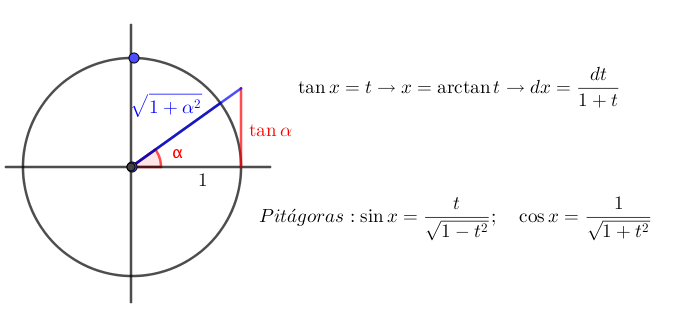
\includegraphics[width=1\textwidth]{imagenes/imagenes07/T07IM03.png}
		\caption{Recordatorio del cambio $x=\tan t$}
	\end{figure}
 
 
 \hspace{5mm} $ \text{---} \qquad$ Cualquier otro caso, usaremos el `cambio general' (sirve para todos los casos, pero no es aconsejable en los anteriores por conducir a integrales racionales más complejas).
 
 Cambio general: $\boxed{\;\tan \frac x 2 = t \;} \; \to \; x=2 \tan t \; \to \;  $ $\boxed{\dd x = \dfrac {2\; \dd t}{1+t^2}}$
 
 Para expresar $\sin x$ y $\cos x$ en función de $t$ nos basamos en las fórmulas:
 
 $\sin 2x= 2 \sin x \; \cos x \;\;  \wedge \;\;  \cos 2x= \cos^2 x - \sin^2 x$, que transformadas convenientemente $(x \leftrightarrow \frac x 2)$ se transforman en: $\sin x = 2 \sin \frac x 2 \; \cos \frac x 2 \; \; \wedge \; \; \cos x= \cos^2 \frac x 2 - \sin^2 \frac x 2\; $. De aquí:
 
 $\boxed{\sin x =} $ $\dfrac {2\sin \frac x 2 \cos \frac x 2 }{\sin^2 \frac x 2 + \cos^2 \frac x 2} \cdot \dfrac {1/\cos^2 \frac x 2}{1/ \cos^2 \frac x 2} = \dfrac {2 \tan \frac x 2}{1 + \tan^2 \frac x 2} $ $\boxed{= \dfrac {2t}{1+t^2}}$
 
  
 $\boxed{\cos x = }$ $ \dfrac {\cos^2 \frac x 2 - \sin^2 \frac x 2 }{\sin^2 \frac x 2 + \cos^2 \frac x 2} \cdot \dfrac {1/\cos^2 \frac x 2}{1/ \cos^2 \frac x 2} = \dfrac {1- \tan^2 \frac x 2}{1 + \tan^2 \frac x 2} $ $\boxed{ = \dfrac {1-t^2}{1+t^2}}$
 
 Obviamente, si aparece $\tan x= \dfrac {\sin x}{\cos x} = \dfrac {2t}{1-t^2}$
 
\subsection{Integración de irracionales algebraicas con cambios trigonométricos}

$\circ \quad  \displaystyle \; \int \mathcal {R} \left (x,\sqrt{a^2-b^2x^2}  \right) \; \dd x \; \to \; $ $\boxed{\; x= \frac a b \; sin t \; }$

$\circ \quad  \displaystyle \; \int \mathcal {R} \left (x, \sqrt{b^2x^2-a^2}  \right) \; \dd x \; \to \; $ $ \boxed{\; x= \frac a b \sec t \;} $

$\circ \quad  \displaystyle \; \int \mathcal {R}  \left ( x, \sqrt{a^2x^2+b^2} \right) \; \dd x \; \to \; $ $ \boxed{\; x=\frac a b \tan t \;} $

\vspace{3mm}

\emph{\textbf{ATENCIÓN: !`Hay que acordarse de deshacer el cambio de variable al final del proceso, en todos los casos!}}

%. $ \left[ \begin{matrix} 1 \\ 2 \end{matrix} \right] $. CV


\begin{ejem}
 
$ \displaystyle \int \dfrac {\sqrt[3]{x-1}+x-1}{\sqrt{(x-1)^3}} \; \dd x  =\; \to \text { CV: }  
\left[ \begin{matrix} x-1=t^6 \leftrightarrow x=1+t^6 \\ \dd x = 6 t^5 \dd t  \end{matrix} \right] \to   $

$ = \displaystyle \int \dfrac {\sqrt[3]{t^6} + t^6}{\sqrt{(t^6)^3}} \; 6t^5\; \dd t = \displaystyle \int \dfrac {t^2+t^6}{t^9} \; 6t^5\; \dd t= 6 \int \left( \dfrac {1}{t^2} + t^2   \right) \; \dd t =  6 \int  (t^{-2} + t^2)\; \dd t= \dfrac {-6}{t}+2t^3=\; $ [Deshacemos el CV] $\; = -\dfrac {6}{\sqrt[6]{x-1}}+ 2 \sqrt[6]{(x-1)^3}+\mathcal C =  -\dfrac {6}{\sqrt[6]{x-1}}+ 2 \sqrt{(x-1)}+\mathcal C$
	
\end{ejem}


\begin{ejem}

$ \displaystyle \int \dfrac {e^{-x}}{1+e^{-x}}\; \dd x =\; $ [aunque es una integral claramente inmediata, la trataremos mediante un CV] $ \to \; \left[ \begin{matrix} t=e^{-x} \\ \dd t = e^{-x}(-1)\dd x \leftrightarrow  \dd x= -\frac {\dd t}{t} \end{matrix} \right]\; \to  $

$\; = \displaystyle \int \dfrac {\cancel{t}}{1+t} \; \dfrac {- \dd t}{\cancel{t}} = - \int \dfrac {1}{1+t} \; \dd t = - \mathrm{ln}|1+t| =\; $ [Deshacemos el CV (cambio de variable)] $\; = \mathrm{ln} (1+e^{-x}) + \mathcal C$

\end{ejem}

\begin{ejem}
$\displaystyle \int \cos^2 (3x) \; \dd x = \;\to  \text { CV: } 	\left[ \begin{matrix} \text{fórmula reducción} \\ \cos^2 \alpha = \frac 1 2 (1 + \cos (2\alpha) \end{matrix} \right] \to  \; [ \cos^2 (3x) = \frac 1 2 (1 + \cos (6x)] \to \; = $
$\frac 1 2  \int (1 + \cos (6x)) \; \dd x = \frac 1 2 \left( x + \dfrac {\sin (6x)}{6}  \right) + \mathcal C$
\end{ejem}

\begin{ejem}
$\displaystyle \int \sin^2 x \; \cos^3 x \; \dd x = [ \text {impar en coseno,  CV: } ] \to $

$\to \left[ \begin{matrix} \sin x = t & \cos x =\sqrt{1-\sin^2 x}= \sqrt{1-t^2}\\ \cos x \dd x = \dd  t & \dd x = \dfrac {\dd t}{\sqrt{1-t^2}} \end{matrix} \right] \to    $	

$\displaystyle \int \;t^2 (\sqrt{1-t^2})^3 \dfrac {\dd t}{\sqrt{1-t^2}} = \int \;t^2 (\sqrt{1-t^2})^2  \dd t = \int t^2(1-t^2) \dd t= \int (t^2-t^4)\dd t= \frac {t^3}{3} - \frac {t^5}{5} \; [ \text { Deshacer el C.V. }] = \dfrac {\sin^3 x}{3}-\dfrac {\sin^5 x}{5}+\mathcal C$
\end{ejem}

\begin{ejem}
	$\displaystyle \int \dfrac {\sin^3 x}{\cos^2 x} \; \dd x = \; $ [La integral es impar en $\sin x$, si llamas $f$ al integrando y reemplazas el `$\sin x$' por `$-\sin x$', obtienes $-f$. El cambio adecuado en este caso es $\cos x = t ] $
	
	$\to \text{CV: } \left[ \begin{matrix} t=\cos x & \sin x=\sqrt{1-t^2} \\ \dd t = -\sin x \dd x & \dd x = - \dfrac {\dd t}{\sqrt{1-t^2}} \end{matrix} \right] \to \displaystyle \int \dfrac {(\sqrt{1-t^2})^3}{t^2} \left(- \dfrac {\dd t}{\sqrt{1-t^2}} \right)   =    $
	
	$\displaystyle - \int \dfrac {1-t^2}{t^2} \dd t = - \int (t^{-2} - 1) \dd t = -(-\frac 1 t - t)= [\text{ Deshacer CV}] = \dfrac {1}{cos x} + \cos x + \mathcal C$	
	
\end{ejem}

\begin{ejem}
$\displaystyle \int \dfrac {\cos x \; \dd x} {\cos^2 x - 2\sin x}=\; $ [si cambiamos  `$\cos x$' por `$-\cos x$', el integrando cambia de signo, la integral es impar en coseno: CV: $\sin x=t \; $]

$\to \left[ \begin{matrix} \sin x = t & \cos x =\sqrt{1-\sin^2 x}= \sqrt{1-t^2}\\ \cos x \dd x = \dd  t & \dd x = \dfrac {\dd t}{\sqrt{1-t^2}} \end{matrix} \right] \to  =\displaystyle \int \dfrac {\cancel{\sqrt{1-t^2}}}{(\sqrt{1-t^2})^2-2t} \left( \dfrac {\dd t}{\cancel{\sqrt{1-t^2}}} \right)  = \int \dfrac {\dd t}{1-2t-t^2}=- \int \dfrac {\dd t}{t^2+2t-1}= \to  $ [Integral racional: no hay que dividir. Busquemos las raíces del denominador.]

	$t^2+2t-1=0 \to x=-1\pm \sqrt{2} \to \dfrac {1}{t^2+2t-1} = \dfrac {A}{t-(-1+\sqrt
	{2})}+\dfrac {B}{t-(-1-\sqrt{2})}=\dfrac {A(t-(-1-\sqrt{2})+B(t-(-1+\sqrt{2}))}{t^2+2t-1} \to $ Identificando coeficientes de los numeradores: $\; 1= A(t+1+\sqrt{2})+B(t+1-\sqrt{2}))$
	
	$ \to \left[ \begin{matrix} t=-1+\sqrt{2}; & 1=A 2\sqrt{2};  & A= \dfrac {1}{2\sqrt{2}}\\
	 t=-1-\sqrt{2}; & 1= B(-2\sqrt{2}); &  B= \dfrac {1}{2\sqrt{2} } \end{matrix} \right] \to $
	 
	 
	$ \to =\displaystyle - \int \dfrac {\dd t}{t^2+2t-1}= - \int \dfrac { \frac { \sqrt{}2 }{ 4 } }{  t+1-\sqrt{2} } \; \dd t  + \int \dfrac { \frac { \sqrt{}2 }{ 4 } }{  t+1+\sqrt{2} } \; \dd t  =\;  $
	
	$= \displaystyle \frac {\sqrt{2}}{4} \left( -\mathrm{ln} (t+1-\sqrt{2}) + \mathrm{ln} (t+1+\sqrt{2}) \right)=\; \text { Desh. CV}; = \displaystyle \frac {\sqrt{2}}{4} \mathrm {ln}\left| \dfrac  {(t+1+\sqrt{2})}  {(t+1-\sqrt{2})} \right| =\frac {\sqrt{2}}{4} \mathrm {ln}\left| \dfrac  {(\sin x +1+\sqrt{2})}  {(\sin x+1-\sqrt{2})} \right| + \mathcal C $	
\end{ejem}


\begin{ejem}
$\displaystyle \int \sqrt{9-x^2} \; \dd x = \; \to $[Integral  irracionales algebraicas de cambios trigonométricos.] =$ \displaystyle\left[ \begin{matrix} x=3\sin t \leftrightarrow t=\arcsin (x/3) \\
\dd x = 3 \cos t  \;  \dd t \end{matrix} \right] \to\;  =  \int \sqrt{9-x^2} \; \dd x =\int \sqrt{9-9\sin^2 t} \; 3 \cos x \dd t = 3 \cdot 3 \; \int cos^2 t \; \dd t = \to  \left[ \text{fórmula reducción: } \;  \cos^2 \alpha = \frac 1 2 (1 + \cos (2\alpha) \right] \to = 9\; \frac 1 2  \int  (1 + \cos 2t) \; \dd t = \frac 9 2 \left( t+\frac 1 2 \sin (2t)   \right) = \frac 9 2 t + \frac 9 4 (2 \sin t \; cos t) =  \frac 9 2 t + \frac 9 4 (2 \sin t \; \sqrt{1-sin^2 t}) = \; \text { [Desh. CV  ] }\; =  \frac 9 2 \; \arcsin (x/3) + \frac 9 4 (2 \sin (\arcsin (x/3))  \; \sqrt{1-sin^2 (\arcsin (x/3) )})  + \mathcal C= \frac 9 2 \; \arcsin (x/3) +\frac 9 2 \; \frac x 3 \; \sqrt{1-\dfrac {x^2}{9}} + \mathcal C =  \frac 9 2 \; \arcsin (x/3) + \frac 1 2 x\; \sqrt{9-x^2} + \mathcal C$

\end{ejem}

\subsection{Ejercicios del método de sustitución (cambio de variable)}

\subsubsection{Ejercicios resueltos del método sustitución}

!`Antes de empezar: comprobar que no tenemos una integral inmediata!. 

\begin{ejer} Resuelve las siguientes integrales:
\begin{multicols}{2}
	
\begin{enumerate}[a) ]

\item $\displaystyle \int \dfrac {3^x}{1+9^x} \; \dd x$

\item $\displaystyle \int \dfrac {1}{x-\sqrt{x}} \; \dd x$

\item $\displaystyle \int \dfrac {1}{(3-x)\sqrt{2-x}} \; \dd x$

\item $\displaystyle \int \dfrac {1}{x\sqrt{1-\mathrm{ln}x}} \; \dd x$ 

\item $\displaystyle \int \sin^4 x \; \cos^3 x \; \dd x$

\item $\displaystyle \int \sin^4 x \; \dd x$

\item $\displaystyle \int \dfrac {\cos^2 x}{1+\sin^2 x} \; \dd x$

\item $\displaystyle \int \dfrac {\sin x + \cos x}{1-\sin x} \; \dd x$

\item $\displaystyle \int \sqrt{1-x^2} \; \dd x$

\item $\displaystyle \int \dfrac{x^3}{\sqrt{4-x^2}} \; \dd x$

\item $\displaystyle \int x\sqrt{1-x^2} \; \dd x$

\item $\displaystyle \int \dfrac{\sqrt{9-x^2}}{x} \; \dd x$

\item $\displaystyle \int \sin3x \; \cos 8x  \; \dd x$

\scriptsize{$\text {Transformación de productos en sumas, apéndice \ref{Kit}  } $} \normalsize{.}
	
\end{enumerate}

\end{multicols}

\end{ejer}

% \left[ \begin{matrix}  \\  \end{matrix} \right] 

\begin{proofw}\renewcommand{\qedsymbol}{$\diamond$}	 
	
\hspace{7mm} $a) \quad \displaystyle \int \dfrac {3^x}{1+9^x} \; \dd x =\text { CV: } \to  \left[ \begin{matrix} 3^x=t \leftrightarrow 9^x=(3^x)^2=t^2 \\ 3^x \; \mathrm{ln}3\; \dd x = \dd t \leftrightarrow \dd x = \dfrac {\dd t}{t \; \mathrm{ln}3}  \end{matrix} \right] \to =  \displaystyle \int \dfrac {\cancel{t}}{1+t^2} \cdot \dfrac {\dd t}{\cancel{t} \; \mathrm{ln}3} =  \dfrac {1}{\mathrm{ln} 3} \int \dfrac {\dd t}{1+t^2}=\dfrac {1}{\mathrm{ln} 3} \arctan t= \dfrac {1}{\mathrm{ln}3} \arctan 3^x + \mathcal C$

\vspace{4mm}
$b) \quad \displaystyle \int \dfrac {1}{x-\sqrt{x}} \; \dd x = \text { CV: } \to \left[ \begin{matrix} x=t^2 \\ \dd x =2 t \dd t \end{matrix} \right] \to \;  =  \int \dfrac {2 t \dd t}{t^2 -t}=$

$= \text {[ factor común en denominador ]} = \int \dfrac {2  \dd t}{t -1}= 2 \mathrm{ln} |t-1|=2 \mathrm{ln} |\sqrt{x}-1|+\mathcal C$	

\vspace{4mm}
$c) \quad \displaystyle \int \dfrac {1}{(3-x)\sqrt{2-x}} \; \dd x = \text { CV: } \to \left[ \begin{matrix}2-x=t^2 \leftrightarrow x=2-t^2  \\  \dd x = -2 \; t \;  \dd t \end{matrix} \right] \to =$

$=\int \dfrac {1}{[3-(2-t^2)] t}\; (-2)t\; \dd t = -2 \int \dfrac {\cancel{t}\; dt}{\cancel{t}(1+t^2)} = -2 \arctan t = -2 \arctan {\sqrt{2-x}}$

\vspace{4mm}
$d) \quad \displaystyle \int \dfrac {1}{x\sqrt{1-\mathrm{ln}x}} \; \dd x  = \text { CV: } \to \left[ \begin{matrix}
 1-\mathrm{ln} x = t \leftrightarrow x=e^{1-t} \\ 
 \dd x = - e^{1-t} \; \dd t 
 \end{matrix} \right]  \; \to \; = $

 $\text{ [ Pero, esta integral es `inmediata' ] } =\displaystyle (-1)\; \int (-1)\; \dfrac {1}{x}\; (1-\mathrm{ln}x)^{-1/2} \; \dd x =$
 
 $=- \dfrac {(1-\mathrm{ln}x)^{+/2}}{1/2} +\mathcal C = -2 \sqrt{1-\mathrm{ln}x}+\mathcal C$	

\vspace{4mm}
$e) \quad \displaystyle \int \sin^4 x \; \cos^3 x \; \dd x= = \text { CV: } \to \; \left[ \begin{matrix}  
    \sin x =t \leftrightarrow x=\arcsin t        \\  
    \dd x = \dfrac {\dd t}{\sqrt{1-t^2}}
   \end{matrix} \right] \; \to \; =$
   
   $= \int t^4 \; (\sqrt{1-t^2})^3 \; \dfrac {\dd t}{\sqrt{1-t^2}} = \int t^4 \; (1-t^2)\; \dd t= \int (t^4-t^6)\; \dd t = \dfrac {t^5}{5} - \dfrac {t^7}{7}=$
   
   $= \dfrac {\sin^5 x}{5} - \dfrac {\sin^7 x}{7}+\mathcal C$	



\vspace{4mm}
$f) \quad \displaystyle \int \sin^4 x \; \dd x = \int \sin^2 x \;\sin^2 x \; \dd x =\;  \to \text{ [fórmulas de reducción:] } \to $

$\to  \sin^2 x = \frac 1 2 (1-\cos 2x) \; \to \; =\int  \frac 1 2 (1-\cos 2x) \cdot \frac 1 2 (1-\cos 2x)  \; \dd x =$

$= \frac 1 4 \int (1-\cos 2x)^2 \; \dd x = \frac 1 4 \int (1-2\cos 2x + cos^2 2x) \; \dd x \; = \; \to \text{ [fórmulas de reducción:] }\to $

$ \to \cos^2 x = \frac 1 2 (1+\cos 2x) \; \to \; =  \frac 1 4 \int \left( 1-2\cos 2x + (\frac 1 2 (1+\cos 4x) \right) \; \dd x \; =$ 

$=\frac 1 4 \int ( \frac 3 2 - 2 cos 2x +\frac 1 2 \cos 4x)\; \dd x= $
$=\displaystyle \frac 1 4 \left(\frac 3 2 \; x - \sin 2x + \frac 1 8 \cos 4x \right)+\mathcal C$

\vspace{4mm}
$g) \quad \displaystyle \int \dfrac {\cos^2 x}{1+\sin^2 x} \; \dd x = \; \text { par en seno y coseno. CV: } x=\tan t \; \to $

$ \left[ \begin{matrix} \tan x = t \leftrightarrow x=\arctan t & \dd x= \dfrac {\dd t}{1+t^2} \\  
\sin x = \dfrac {t}{\sqrt{1-t^2}} & \cos x = \dfrac {1}{\sqrt{1-t^2}}
\end{matrix} \right] \; \to = \displaystyle \int  
\dfrac
{ \left( \dfrac {1}{\sqrt{1-t^2}}   \right)^2}
{ 1 + \left(  \dfrac {t}{\sqrt{1-t^2}}  \right)^2  }\cdot \dfrac {\dd t}{1+t^2} = \displaystyle \int  
 \dfrac {\dfrac {1}{\cancel{1-t^2}}}{\dfrac {2+t^2 }{\cancel{1-t^2}}}\cdot \dfrac {\dd t}{1+t^2} = \int \dfrac {\dd t}{(2+t^2)(1+t^2)}= \; \text{ integral racional con dos RCS; }\cdots \to = $
 
 $\cdots \; \to \; =\sqrt{2} \arctan (\sqrt{2} \tan x)-x + C$



\vspace{4mm}
$h) \quad \displaystyle \int \dfrac {\sin x + \cos x}{1-\sin x} \; \dd x \; = \to \text { Cambio general. CV:}\; \tan \frac x 2 = t \; \to \; $	

$\to \; \left[ \begin{matrix}
 \tan \frac x 2 = t \leftrightarrow t= 2 \arctan x & \dd x = \dfrac {2 \; \dd t}{1+t^2}        \\  
 \sin x = \dfrac {2t}{1+t^2} & \cos x = \dfrac {1-t^2}{1+t^2}        
 \end{matrix} \right] \; \to $ 
 
 $\displaystyle \int \dfrac {\dfrac {2t }{1+t^2}+\dfrac {1-t^2}{1+t^2}}{1-\dfrac {2t}{1+t^2}} \cdot \dfrac {2 \; \dd t}{1+t^2} =\displaystyle \int \dfrac {\dfrac {2t+1-t^2}{\cancel{1+t^2}}}{\dfrac {1+t^2-2t}{\cancel{1+t^2}}} 
 \cdot \dfrac {2 \; \dd t}{1+t^2} =\displaystyle \int \dfrac {-t^2+2t+1}{t^2-2t+1} \cdot \dfrac {2 \; \dd t}{1+t^2} = \; \to $
 
 $\to\; \text {dividiendo el integrando } \; \to \; = \displaystyle \int \left( -1 + \dfrac {2}{ (t-1)^2}  \right) \cdot \dfrac {2\dd t}{1+t^2} = $
 
$=  -\int \dfrac {2 \dd t}{ 1+t^2} + 4 \int \dfrac {\dd t} {(t-1)^2 \cdot  (1+t^2)} = - \arctan t + \text {Inr Racional RRM(2) y RCS } \to \cdots \to =  \dfrac {2 \sin x/2}{\cos x/2 - \sin x/2}-2\; \mathrm{ln} \left|\cos x/2 - \sin x/2  \right| +\mathcal C$

\vspace{4mm}
$i) \quad \displaystyle \int \sqrt{1-x^2} \; \dd x \to \; [\text { CV: } \; sin x =t]\;  \to  \left[ \begin{matrix}
	x = \sin t   \\
	\dd x = \cos t \; 	\dd t 
	
	\end{matrix} \right] \; \to \; =\displaystyle \int \sqrt{1-\sin^2 t}\; \cos t \; \dd t = \int  \cos^2 t \; \dd t=\to [\text { fórmula de reducción: }\cos^2 t = \frac 1 2 (1 + \cos 2t)\;  ] \to \; = \frac 1 2\int (1+\cos 2t ) \; \dd t= \dfrac t 2 - \dfrac {\sin 2t }{4}= \dfrac t 2 - \dfrac {2\sin t\; cos t }{4}= [\text { Desh. CV }] = \dfrac {arcsin x}{2} - \frac 1 2 x \sqrt{1-x^2} + \mathcal C \qquad \qquad $
	
	$\textcolor{gris}
	{\text {hemos usado: }  \cos t = \sqrt{1-\sin^2 t}=\sqrt {1- (\arcsin(sin x))^2} = \sqrt{1-x^2} } $  


\vspace{4mm}
$j) \quad \displaystyle \int \dfrac{x^3}{\sqrt{4-x^2}} \; \dd x \to \; [\text { CV: } \; 2sin x =t]\;  \to \left[ \begin{matrix}
	x = 2\sin t \leftrightarrow t=\arcsin (x/2)  \\
	\dd x = 2\cos t \; 	\dd t   
	\end{matrix} \right] \; \to \; =$	
	
$\displaystyle \int \dfrac {8\sin^3 t}{ \sqrt{4(1-\sin^2 t)}}  \; 2 \cos t\; \dd t  = 16 \int  \dfrac { \sin^3 t \; \cancel{cos t} }{2\; \cancel{\cos t}} \; \dd t = 8 \int \sin^3 t \; \dd\; t = \to \; $

$[\text { CV: } \; 
cos t =z]\;  \to \left[ 
\begin{matrix} 
\cos t = z \leftrightarrow t= \arccos z \\
 -\sin t \; \dd t \leftrightarrow \dd t = \dfrac {- \dd z}{\sqrt{1-z^2}}
 \end{matrix} 
\right] 
\; \to \; =\displaystyle 8 \int ( \sqrt{1-z^2} )^3 \;  \dfrac {- \dd z}{\sqrt{1-z^2}} = -8 \int (1-z^2) \;\dd z = -8z + \dfrac {8z^3}{3} =\; \to \text {Desh. CV }\; \to = -8 \cos t + \dfrac {8 \cos^3 t }{3 } =\; \to \text {Desh. CV }\; \to =   -8 \cos (arcsin (x/2)) + \dfrac {8 \cos^3 (arcsin (x/2)) }{3 } + \mathcal C= \cdots = \dfrac { \sqrt{(4-x^2)^3} }{3}-4 \sqrt{4-x^2}+ \mathcal C$

\vspace{4mm}
$k) \quad \displaystyle \int x\sqrt{1-x^2} \; \dd x = \; \to \;  [\text { CV: } \; sin x =t]\;  \to  \left[ \begin{matrix}
	x = \sin t   \\
	\dd x = \cos t \; 	\dd t 
	\end{matrix} \right] \; \to \; =
	\int \sin t \; (\cos t)^2 \; \dd t = [\text { inmediatas }] = \dfrac {\cos^3 t} {3} = \dfrac {\sqrt {(1-x^2 )^3}}{3} + \mathcal C$	

\vspace{4mm}
$l) \quad \displaystyle \int \dfrac{\sqrt{9-x^2}}{x} \; \dd x =  \; \to \;  [\text { CV: } \; x=3 \sin t]\;  \to  \left[ \begin{matrix}
	x= 3 \sin t  \\
	\dd x = 3 \cos t \; 	\dd t 
	\end{matrix} \right] \; \to \; =$
	
	$= \int \dfrac{\sqrt{9-9 \sin^2 t}}{3 \sin t } \; 3 \cos t \dd t = 
	3\int \dfrac {\cos^2 t}{\sin t }\; \dd t = \; \to \; [\text {impar en } \sin t \text{  CV: } \;  \cos t =z]\;  \to \left[ \begin{matrix} \cos t = z \leftrightarrow t= \arccos z  \\ -\sin t \; \dd t = \dd z \leftrightarrow \dd t = \dfrac {-\dd z}{ \sqrt{1-z^2} } \ \end{matrix} \right] \; \to \; = 3\int \dfrac {z^2}{\sqrt{1-z^2}} \; \dfrac {- \dd z}{\sqrt{1-z^2}}=  3 \int \dfrac {\textbf{+1}-z^2\textbf{-1}}{1-z^2} \; \dd z = 3\int \left( 1- \dfrac {-1}{1-z^2} \right)\; \dd z = 3z + \frac 3 2 \arctan z = 3\cos t + \frac 3 2 \arctan (\cos t)=
	3 \cos (\arcsin (x/3)) + \frac 3 2 \arctan (\cos (\arcsin (x/3))) + \mathcal C \qquad$ 
	
	\textcolor{gris}{ Lo dejamos ahí ...}

\vspace{4mm}
$m) \quad \displaystyle \int \sin3x \; \cos 8x  \; \dd x =\; \to $

\textcolor{gris}{\hspace {10mm} Transformación de productos en sumas, apéndice \ref{Kit}}

\textcolor{gris}{\hspace {10mm}$\sin a \cdot \cos b= \dfrac 1 2 [\sin(a+b)+\sin(a-b)]$}

\textcolor{gris}{\hspace {10mm} $\sin 3x \cdot \cos 8x = \frac 1 2 [ \sin (11x/2) + \sin (-5x/2)]= \frac 1 2 [ \sin (11x/2) - \sin (5x/2)]$}

$\to \; = \displaystyle \frac 1 2 \cdot \frac  {2} {11} \int \frac {11} {2}\;  \sin(11x/2)\; \dd x + \frac 1 2 \cdot \frac 2 5 \; \int  \frac 5 2  \; \sin (5x/2) \; \dd x =$

$=\displaystyle -\frac {1}{22} \cos (11x/2) - \frac {1}{5} \cos (5x/2)+\mathcal C$
	
\end{proofw}

\subsubsection{Ejercicios propuestos del método sustitución}

\begin{enumerate}[a) ]

\item $\displaystyle \int  \sin^3 x \cos^{15} x \; \dd x \quad $ 
\textcolor{gris}{Sol: $  +\mathcal C$}

\item $\displaystyle \int \dfrac {\cos x}{\sin x + \cos x}  \; \dd x \quad $ 
\textcolor{gris}{Sol: $ \dfrac {x+\sqrt{x}}{\sqrt{x}+\sqrt[4]{x}} +\mathcal C$}

\item $\displaystyle \int  \dfrac {1+x+\sqrt{x+1}}{(x+1)\cdot \sqrt[3]{x+1}} \; \dd x \quad $ 
\textcolor{gris}{Sol: $  +\mathcal C$}

\item $\displaystyle \int  \dfrac {e^{3x}}{3^{2x}-3 e^x+2} \; \dd x \quad $ 
\textcolor{gris}{Sol: $  +\mathcal C$}

\item $\displaystyle \int  \dfrac {1}{x^4 \sqrt{x^2-1}} \; \dd x \quad $ 
\textcolor{gris}{Sol: $  +\mathcal C$}

\item $\displaystyle \int  \dfrac {1}{3+\cos x + 2\sin x} \; \dd x \quad $ 
\textcolor{gris}{Sol: $  +\mathcal C$}

\item $\displaystyle \int  \sin ( \mathrm{ln }x ) \; \dd x \quad $ 
\textcolor{gris}{Sol: $  +\mathcal C$}

\item $\displaystyle \int  \dfrac {1}{x \sqrt{x^2+2x-3}} \; \dd x $ 
\textcolor{gris}{Sol:Usa el método de Herón  }

\item $\displaystyle \int \sin x \; \cos 2x \; cos 3x \; \dd x  $
\textcolor{gris}{Sol:Transformación de productos en sumas, apéndice \ref{Kit} }

\end{enumerate}

\vspace{4mm}
\emph{Existen muchos métodos más de integración, pero para los objetivos del curso, no veremos más.}

\section{Cálculo de primitivas bajo determinadas condiciones}

%$\left[ \begin{matrix} 1 & 2\\ 3 & 4\end{matrix} \right]$

\begin{ejem}
Determina la función $f(x)$, sabiendo que $f''(x)=x\; \mathrm{ln} x; \; f'(1)=0; \; f(e)=4$	

\vspace{3mm} 

$ \displaystyle f'=\int f'' \dd x; \quad f = \int f' \dd x$  

$ f'(x) = \displaystyle \int f''  \dd x = \int x\; \mathrm{ln} x \dd x =\;  $ [PARTES] $\; = \left[ \begin{matrix} u= \mathrm{ln} x & \to &  \dd u = \frac 1 x \dd x\\ 
v=x\; \dd x & \to & v= \frac {x^2}{2} 
 \end{matrix} \right] = \frac {x^2}{2} \mathrm{ln} x - \frac 1 2 \int x \dd x = \frac {x^2}{2} \mathrm{ln} x  -\frac {x^2}{4} + \mathcal C $
 
 Imponiendo la condición de que $f'(1)=0 \to f(1)=-\frac 1 4 + \mathcal C =0 \to \mathcal C=\frac 1 4; $. Con lo que nuestra función $f'$ es:  $\; f'(x)= \frac {x^2}{2} \left(  \mathrm{ln} x  -\frac {1}{2}\right)+\frac 1 4 $ 
 
 $\displaystyle f = \int f' \dd x = \int \frac {x^2}{2}  \left[ \left(  \mathrm{ln} x  -\frac {1}{2}\right) + \frac 1 4 \right] \dd x = \cdots = \to $ La primera integral (la del paréntesis) también la integramos por partes llamando $u$ a la parte logaritmica. Se obtiene:
 
  $\cdots \; \to \; = \displaystyle \frac {x^6}{6} \left( \mathrm{ln} x - 1  \right) - \frac {x^3}{18} + \frac {x}{4} + \mathcal K$, que imponiendo la condición de partida , $f(e)=4$, nos lleva, por fin, a: $\cdots \to \mathcal K=-\frac {e^3}{36}\; $ y la primitiva buscada es:
  
  $f(x)= \displaystyle \frac {x^6}{6} \left( \mathrm{ln} x - 1  \right) - \frac {x^3}{18} + \frac {x}{4} - \frac {e^3}{36}$
\end{ejem}

\begin{ejem}
Determina $y=f(x), \; x>-1$ sabiendo que $y'=\dfrac {a}{1+x}$ y que $f(0)=1 \; \wedge \; f(1)=-1$	

\vspace{3mm} 

$\displaystyle f(x)=\int f'(x) \; dd x= \int \dfrac {a}{1+x} \; \dd x= a \mathrm{ln} (1+x)+\mathcal C\; \; $ \textcolor{gris}{Usamos paréntesis y no valor absoluto en el argumento del logaritmo por la condición inicial $x>-1$}


Imponiendo ahora las condiciones iniciales $f(1)=0$ y $f(e)=4$, se obtiene fácilmente el resultado: $\mathcal C=1$ y $a= \frac {-1}{\mathrm{ln}2}$. La función $f$ buscada es:
$f(x)=-\frac {2}{ \mathrm{2} }\; \mathrm {ln} (1+x) + 1$

\end{ejem}

\begin{ejem}
Encuentra la función derivable $f:[-1,1]\to \mathbb R$, que cumple $f(1)=-1$ y tal que 
$f'(x)=\begin{cases}
x^2-2x & \text{ si } -1\le x <0 \\
e^x-1 & \text{ si } 0\le x \le 1	
\end{cases}$

\vspace{3mm}

$\displaystyle f(x)= \int f'(x) \dd x = 
\begin{cases}
 \int (x^2-2x)\dd x = \frac {x^3}{3}	 - x^2 \mathcal C_1 & 1-\le x < 0 \\
\int (e^x-1) \dd x = e^x -x + \mathcal C_2 & 0\le x \le 1
\end{cases}$

Determinaremos $\mathcal C_1$ y  $\mathcal C_2$ teniendo en cuenta la condición inicial de que $f(1)=-1$ y que $f$ es derivable, ergo $f$ es continua en $x=0$. Imponiendo estas dos condiciones se obtiene:  $\mathcal C_1=1-e$ y  $\mathcal C_2=-e$. La función buscada es:


$\displaystyle f(x) =
\begin{cases}
\frac {x^3}{3}	 - x^2 +1-e & 1-\le x < 0 \\
 e^x -x -e & 0\le x \le 1
\end{cases}$

\end{ejem}

\begin{ejem}
Halla una primitiva $F(x)$ de la función $f(x)=3x^2-6x$ tal que $F(x)$ tenga un mínimo en el punto $(2,0)$. Determina los demás extremos relativos de $F(x)$

\vspace{3mm}

$\displaystyle F(x)= \int f(x) \dd x = \int (3x^2-6x)\dd x= x^3-3x^2+\mathcal C$

La función $F$ tiene un mínimo en $(2,0)$, luego pasa por $(2,0) \quad F(2)=0 \to \mathcal C=4$. La función buscada es:

$F(x)=x^3-3x^2+4$. Busquemos sus PC($F'=f=3x^2-6x$). Como $F'$ existe siempre, buscamos cuando $F'=0 \to x=0 \; \wedge \; x=2$

Estudiando el signo de $F'$  a la izqda. y dcha. de los PC, encontramos: $F$ tiene un $M(0,4)$ y un $m(2,0)$.

\end{ejem}

\emph{Al final de la próxima sección, se proponen ejercicios de integrar funciones a trozos y de calculo de primitivas sujetas a determinadas condiciones.}



\section{Ejercicios propuestos finales}

Existen muchos métodos más de integración, pero para los objetivos del curso, no veremos más.

!`Antes de empezar: comprobar que no tenemos una integral inmediata y no mires el resultado antes de intentar resolverla!. 

\leqnomode
\renewcommand{\theequation}{\arabic{equation}}
\setcounter{equation}{0}
\begin{fleqn}

\subsection*{Inmediatas}
	
	\begin{equation}
		\int (x+\sqrt {x})  \: \mathrm{d} x = \textcolor{gris}{\frac{x^2}{2} +\frac {2x\sqrt{x}}{3}+ \mathcal C}
	\end{equation}
	
	\begin{equation}
		\int \left( \frac {3}{\sqrt x} - \frac {x\sqrt x}{4} \right)\mathrm{d}x=\textcolor{gris}{6\sqrt x - \frac 1 {10} x^2 \sqrt x + \mathcal C}
	\end{equation}	

	\begin{equation}
		\int \left(\frac 1 {x^2}+ \frac 4 {x\sqrt x}+2 \right)\mathrm{d}x=\textcolor{gris}{-\frac 1 x - \frac 8 {\sqrt x}+2x + \mathcal C}
	\end{equation}
	\begin{equation}
		\int {\left(2x^3+\frac 1 {\sqrt[4]x} \right)}^2 \mathrm{d}x=\textcolor{gris}{\frac {4x^7}{7}+ \frac {16} {5} x \sqrt[4]{x}+2\sqrt {x}+\mathcal C}
	\end{equation}
	%5
	\begin{equation}
	\int e^{5x}\mathrm{d}x=\textcolor{gris}{\frac 1 5 e^{5x}+\mathcal C} 	
	\end{equation}
	\begin{equation}
		\int \sin \:ax\:\mathrm{d}x=\textcolor{gris}{-\frac {-\cos \: ax}{a}+\mathcal C}
	\end{equation}
	\begin{equation}
		\int \frac {\mathrm{ln}\:2x}{3x}\:\mathrm{d}x=\textcolor{gris}{\frac 1 6 \: \mathrm{ln}^2 |2x| + \mathcal C}
	\end{equation}
	\begin{equation}
		\int  \frac {\mathrm{d}x} {5x+8} =\textcolor{gris}{ \frac {1} {5}  \;\mathrm{ln} \abs{5x+8}+\mathcal C}
	\end{equation}
	\begin{equation}
		\int \tan \: 2x \: \mathrm{d}x =\textcolor{gris}{ -\frac 1 2 \; \mathrm{ln} \abs{\cos\: 2x}+\mathcal C}
	\end{equation}
	%10
	\begin{equation}
		\int \sin^2x\cdot \cos\:x\:\mathrm{d}x=\textcolor{gris}{\frac{\sin^3 x}{3}+\mathcal C}
	\end{equation}
	\begin{equation}
		\int \sqrt{x^2 +3} \cdot x\:\mathrm{d}x=\textcolor{gris}{\frac 1 3 \sqrt{{(x^2+3)}^3}+\mathcal C}
	\end{equation}
	\begin{equation}
		\int \frac{x^2 \mathrm{d}x}{\sqrt{x^3+1}}=\textcolor{gris}{\frac 2 3 \sqrt{x^3+1}+\mathcal C}
	\end{equation}
	\begin{equation}
		\int \frac{\sin\:x}{\cos^2x}\mathrm{d}x=\textcolor{gris}{\frac 1 {\cos\:x}+\mathcal C}
	\end{equation}
	\begin{equation}
		\int \frac{\tan\:x}{\cos^2x}\mathrm{d}x=\textcolor{gris}{\frac{\tan^2x}{2}+\mathcal C}
	\end{equation}
	%15
	\begin{equation}
		\int \frac{3 \mathrm{d}x}{\cos^2x\cdot \sqrt{\tan\:x-1}}=\textcolor{gris}{6\sqrt{\tan\:x-1}+\mathcal C}
	\end{equation}
	\begin{equation}
		\int \frac{\cos\: 5x}{(1-\sin\: 5x)^2}\mathrm{d}x=\textcolor{gris}{-\frac{1}{5(1-\sin\: 5x)}+\mathcal C}
	\end{equation}
	\begin{equation}
		\int \frac{\sin\: 3x}{\sqrt [3]{\cos^4 3x}}\mathrm{d}x=\textcolor{gris}{\frac{1}{\sqrt [3]{\cos\: 3x}}+ \mathcal C}
	\end{equation}
	\begin{equation}
		\int \frac{\arcsin\:x}{\sqrt{1-x^2}}\mathrm{d}x=\textcolor{gris}{\frac 1 2 \arcsin^2 x+\mathcal C}
	\end{equation}
	\begin{equation}
		\int \frac{\arctan^3\: x}{1+x^2}\mathrm{d}x=\textcolor{gris}{\frac 1 4 \arctan^4 x+\mathcal C}
	\end{equation}
	%20
	\begin{equation}
		\int \frac{\mathrm{d} x}{\cos^2 x \cdot (3\: tan\: x+1)}=\textcolor{gris}{\frac 1 3 \mathrm{ln} \abs{3\: \tan\: x+1}+\mathcal C}
	\end{equation}
	\begin{equation}
		\int \frac{\mathrm{d}x}{\sqrt{1-4x^2}\cdot \arcsin\: 2x}\textcolor{gris}{= \frac 1 2 \mathrm{ln} \abs{\arcsin \: 2x}+\mathcal C}
	\end{equation}
	\begin{equation}
		\int e^{\sin\: x}\cos\: x\: \mathrm{d}x=\textcolor{gris}{e^{\sin\:x}+\mathcal C}
	\end{equation}
	\begin{equation}
		\int e^{3x^2-6x+5}\cdot (x-2)\: \mathrm{d}x=\textcolor{gris}{\frac 1 6 e^{3x^2-6x+5}+\mathcal C}
	\end{equation}
	\begin{equation}
		\int \frac{e^x \: \mathrm{d}x}{3+4e^x}=\textcolor{gris}{\frac 1 4 \mathrm{ln} (3+4e^x)+\mathcal C}
	\end{equation}
	%25
	\begin{equation}
		\int \frac{\mathrm{d}x}{5+10x^2}=\textcolor{gris}{\frac{1}{5\sqrt{2}}\: \arctan(\sqrt{2}\: x)+\mathcal C}
	\end{equation}
	\begin{equation}
		\int \frac{\mathrm{d}x}{\sqrt{1-3x^2}}=\textcolor{gris}{\frac{1}{\sqrt{3}}\: \arcsin(\sqrt{3}\:x)+\mathcal C}
	\end{equation}
	\begin{equation}
		\int \frac{\mathrm{d}x}{4+x^2}=\textcolor{gris}{\frac 1 2 \: \arctan\frac x 2 +\mathcal C}
	\end{equation}
	\begin{equation}
		\int\frac{x}{\sqrt{1-x^4}}\: \mathrm{d}x=\textcolor{gris}{\frac 1 2 \arcsin\: x^2 + \mathcal C}
	\end{equation}
	\begin{equation}
		\int \frac{\cos\: x}{k^2+\sin^2x}\: \mathrm{d}x=\textcolor{gris}{\frac 1 k\:  \arctan \left( \frac {\sin\: x}{k} \right)+\mathcal C}
	\end{equation}
	%30
	\begin{equation}
		\int \frac{x-\arccos\: x}{\sqrt{1-x^2}\: \mathrm{d}x}=\textcolor{gris}{\frac 1 2 \: (\arccos\: x)^2-\sqrt{1-x^2}+\mathcal C}
	\end{equation}
	
	\subsection*{Integración "por partes"}
	
	\begin{equation}
		\int x\: \mathrm{ln} x \: \mathrm{d}x=\textcolor{gris}{\frac 1 2 \: x^2 \left( \mathrm{ln} x - \frac 1 2 \right) + \mathcal C}
	\end{equation}
	\begin{equation}
		\int x\: \sin\: x \: \mathrm{d}x=\textcolor{gris}{\sin\: x-x\: \cos \: x+\mathcal C}
	\end{equation}
	\begin{equation}
		\int \mathrm{ln} x \: \mathrm{d}x=\textcolor{gris}{x\: (\mathrm{ln} x - 1)+\mathcal C}
	\end{equation}
	\begin{equation}
		\int \arcsin\: x\: \mathrm{d}x=\textcolor{gris}{x\cdot \arcsin\: x+ \sqrt{1-x^2}+\mathcal C}
	\end{equation}
	%35
	\begin{equation}
		\int \mathrm{ln}(5-3x)\mathrm{d}x=\textcolor{gris}{\left(x-\frac 5 3 \right)\:\mathrm{ln}|5-3x| - x +\mathcal C}
	\end{equation}
	\begin{equation}
		\int x^n \mathrm{ln} x \: \mathrm{d}x=\textcolor{gris}{\frac{x^{n+1}}{n+1}\left( \mathrm{ln} x - \frac {1}{n+1} \right) +\mathcal C}
	\end{equation}
	\begin{equation}
		\int x \: \arctan\: x \: \mathrm{d}x\textcolor{gris}{=\frac 1 2 \left[ (x^2+1)\arctan \: x-x \right] + \mathcal C}
	\end{equation}
	\begin{equation}
		\int x\: \arcsin\: x \: \mathrm{d}x=\textcolor{gris}{\frac 1 4 \left[ (2x^2-1)\: \arcsin\: x+ x \: \sqrt{1-x^2} \right] + \mathcal C}
	\end{equation}
	\begin{equation}
		\int \mathrm{ln}(3x^2-7)\: \mathrm{d}x= \textcolor{gris}{x\;\mathrm{ln}(3x^2-7)+ 2\: \sqrt{\frac 7 3} \arctan\: \left( \sqrt{\frac 7 3 } x \right)+\mathcal C}
	\end{equation}
	%40
	\begin{equation}
		\int \mathrm{ln}(1+2x)\: \mathrm{d}x =\textcolor{gris}{\dfrac {2x+1}{2}\left( \mathrm{ln}|2x+1|-1 \right)+\mathcal C}
	\end{equation}
	\begin{equation}
		\int x\: \arctan \: x \: \mathrm{d}x=\textcolor{gris}{\frac 1 2 \left[ (x^2+1)\:\arctan\: x-x\right]+\mathcal C}
	\end{equation}
	\begin{equation}
		\int x \: \arcsin\: x\: \mathrm{d}x=\textcolor{gris}{\frac 1 4 \left[ (2x^2-1)\:\arcsin\: x+x\sqrt{1-x^2} \right] + \mathcal C}
	\end{equation}
	\begin{equation}
		\int x\cdot \sin^2 x\:\mathrm{d}x=\textcolor{gris}{\frac{x^2}{4}-\dfrac {x\; \sin 2x}{4}- \dfrac {\cos 2x}{8}+\mathcal C}
	\end{equation}
	\begin{equation}
		\int \cos(\mathrm{ln} x)\: \mathrm{d}x=\textcolor{gris}{\frac x 2 \: \left( \sin (\mathrm{ln} x)+\cos (\mathrm{ln} x) \right)+\mathcal C}
	\end{equation}
		
	\subsection*{Integrales Racionales}
	
	%45
	\begin{equation}
		\int \frac{\mathrm{d}x}{x^2+2x+5}=\textcolor{gris}{\frac 1 2 \: \arctan \left( \frac{x+1}{2}\right) +\mathcal C}
	\end{equation}
	\begin{equation}
		\int \frac{\mathrm{d}x}{3x^2-2x+1}=\textcolor{gris}{\frac{1}{\sqrt{2}}\: \arctan\frac{3x-1}{\sqrt{2}}+\mathcal C}
	\end{equation}
	\begin{equation}
		\int \frac{5x+1}{5x^2-3x+2}\mathrm{d}x=\textcolor{gris}{\frac{1}{2}\mathrm{ln}(5x^2-3x+2)-\frac{1}{\sqrt{31}}\: \arctan\frac{10x-1}{\sqrt{31}}+\mathcal C}
	\end{equation}
	\begin{equation}
		\int \frac{3x-1}{x^2-x+1}\mathrm{d}x=\textcolor{gris}{\frac{3
	}{2}\mathrm{ln} \abs{x^2-x+1}+\frac{1}{\sqrt{3}}\: \arctan\frac{2x-1}{\sqrt{3}}+\mathcal C}
	\end{equation}
	\begin{equation}
		\int \frac{2x+1}{5x^2-x+2}\mathrm{d}x=\textcolor{gris}{\frac{13}{65}\mathrm{ln} \abs {5x^2-x+2}+ \frac {4\sqrt{39}}{65}\: \arctan \frac{10x-1}{\sqrt{39}}+\mathcal C}
	\end{equation}
	%50
	\begin{equation}
		\int \frac{2x-1}{(x-1)(x-2)} \mathrm{d}x=\textcolor{gris}{\mathrm{ln} \abs {\frac{(x-2)^3}{x-1}}+\mathcal C}
	\end{equation}
	\begin{equation}
		\int\frac{x^5+x^4+1}{x^3-9x}\mathrm{d}x=\textcolor{gris}{\dfrac {x^3}{3} -\dfrac {x^2}{2} +9x+ \frac {163}{18}\mathrm{ln}|x-3|-\frac 1 9 \mathrm{ln}|x|- \frac {323}{18}\mathrm {ln}|x+3|+\mathcal C}
	\end{equation}
	\begin{equation}
		\int \frac{x^4}{(x^2-1)(x+2)}\mathrm{d}x=\textcolor{gris}{\frac{x^2}{2}-2x+\frac{1}{6}\mathrm{ln} \abs{\frac{x-1}{(x+1)^3}}+\frac {16}{3}\mathrm{ln} \abs{x+2}+\mathcal C}
	\end{equation}
	\begin{equation}
		\int \frac{x-8}{x^3-4x^2+4x}\mathrm{d}x=\textcolor{gris}{\frac{3}{x-2}+2\:\mathrm{ln} \frac{x-2}{x}+\mathcal C}
	\end{equation}
	\begin{equation}
		\int \frac{\mathrm{d}x}{x^2(x^2+1)}=\textcolor{gris}{-\frac 1 x - \arctan x +\mathcal C}
	\end{equation}
	%55
	\begin{equation}
		\displaystyle \int \frac{\mathrm{d}x}{x^3+8}=\textcolor{gris}{\frac {1}{24} \; \mathrm{ln} \left| { \left( \dfrac {x-1}{\sqrt{3}}  \right)^2 +1 }  \right|+ \sqrt{3}\arctan \left( \dfrac {x-1}{\sqrt{3}}  \right) +\mathcal C}
	\end{equation}
	
	\subsection*{Integrales irracionales algebráicas}
	
	\begin{equation}
		\int \frac{\sqrt{x}}{\sqrt[4]{x^3}+1}\mathrm{d}x=\textcolor{gris}{\frac 4 3 \: \left[ \sqrt[4]{x^3}-\mathrm{ln} \left( \sqrt[4]{x^3}+1 \right) \right]+\mathcal C}
	\end{equation}
	\begin{equation}
		\int \frac{\sqrt{x^3}-\sqrt[3]{x}}{6\sqrt[4]{x}}	\mathrm{d}x=\textcolor{gris}{\frac{2}{27}\: \sqrt[4]{x^9}-\frac{2}{13}\: \sqrt[12]{x^{13}}+\mathcal C}
		\end{equation}
	\begin{equation}
			\int \frac{\sqrt[6]{x}+1}{\sqrt[6]{x^7}+\sqrt[4]{x^5}}\mathrm{d}x=\textcolor{gris}{-\frac{6}{\sqrt[6]{x}}+\frac{12}{\sqrt[12]{x}}+24\: \mathrm{ln} \abs{\sqrt[12]{x}}-24\: \mathrm{ln} \abs{\sqrt[12]{x}+1}+\mathcal C}
		\end{equation}
	\begin{equation}
			\int \frac{\sqrt x}{1+\sqrt[3]x}\mathrm{d}x=\textcolor{gris}{\frac{6x\sqrt [6]{x}}{7}-\frac{6\sqrt[6]{x^5}}{5}+2\sqrt{x}-6\sqrt[6]x+6\: \arctan\: \sqrt[6]x+\mathcal C}
		\end{equation}
	%60
	\begin{equation}
			\int \frac{1}{2+\sqrt{x+1}}\mathrm{d}x=\textcolor{gris}{2\sqrt{x+1}-4 \mathrm{ln} \abs{2+\sqrt{x+1}}+\mathcal C}
		\end{equation}
	\begin{equation}
			\int \frac{\sqrt{x-1}}{x}\mathrm{d}x=\textcolor{gris}{2\sqrt{x-1}-2 \arctan \sqrt{x-1}+\mathcal C}
		\end{equation}
	\begin{equation}
			\int x\sqrt{1-x^2}\mathrm{d}x=\textcolor{gris}{-\frac{1}{3}\sqrt{{(1-x^2)}^3}+\mathcal C}
		\end{equation}
	\begin{equation}
			\int \frac{\mathrm{d}x}{\sqrt{7-x-x^2}}=\textcolor{gris}{\arcsin \frac{x+3}{4}+\mathcal C}
		\end{equation}
	\begin{equation}
			\int \sqrt {1-x^2}	= \textcolor{gris}{\frac 1 2 \: \arcsin x+\frac 1 2 \: x\:\sqrt{1-x^2}+\mathcal C}			
		\end{equation}
	%65
	\begin{equation}
			\int \frac{\sqrt{9-x^2}}{x} = \textcolor{gris}{\sqrt{9-x^2}+\frac 1 2 \: \mathrm{ln} \abs{\frac{3-\sqrt{9-x^2}}{3+\sqrt{9-x^2}}}+\mathcal C}
		\end{equation}		
	\begin{equation}
			\int \frac{\sqrt{a^2-x^2}}{x^2}	\mathrm{d}x=\textcolor{gris}{	-\frac{\sqrt{a^2-x^2}}{x}-\arcsin \frac x a +\mathcal C}
		\end{equation}
	\begin{equation}
			\int \frac{\mathrm{d}x}{x^2\: \sqrt{1+x^2}}=\textcolor{gris}{-\frac{\sqrt{1+x^2}}{x}+\mathcal C}
		\end{equation}

	\subsection*{Integrales trigonométricas}

	\begin{equation}
		\int \cos^2x\:\mathrm{d}x=\textcolor{gris}{\frac x 2 + \frac 1 4 \sin 2x + \mathcal C}
	\end{equation}
	\begin{equation}
		\int \sin^2 7x \:\mathrm{d}x=\textcolor{gris}{\frac x 2-\frac 1 {28}\sin 14x+\mathcal C }
	\end{equation}
	%70
	\begin{equation}
		\int \sin^2 5x \:\mathrm{d}x\textcolor{gris}{= \frac 1 2 x- \frac 1 {20}\sin 10x+\mathcal C}
	\end{equation}
	\begin{equation}
		\int \cos^3 x \:\mathrm{d}x=\textcolor{gris}{\sin x-\frac{\sin^3 x}{3}+\mathcal C}
	\end{equation}
	\begin{equation}
		\int \cos^3 x \sin^2 x \:\mathrm{d}x=\textcolor{gris}{-\dfrac {1}{\sin x}-\sin x +\mathcal C}
	\end{equation}
	\begin{equation}
		\int \frac{\sin^3 x}{\cos^2 x}\:\mathrm{d}x=\textcolor{gris}{\cos x+\frac{1}{\cos x}+\mathcal C}
	\end{equation}
	\begin{equation}
		\int \sin^3 x \: \cos^2 x \:\mathrm{d}x\textcolor{gris}{=-\frac{\cos^3 x}{3}+\frac{\cos^5 x}{5}+\mathcal C}
	\end{equation}
	%75
	\begin{equation}
		\int \sin^2 x \: \cos^2 x \:\mathrm{d}x=\textcolor{gris}{\frac 1 8 x- \frac 1 {32} \sin 4x + \mathcal C}
	\end{equation}
	\begin{equation}
		\int \sin 4x \: \cos x \:\mathrm{d}x=\textcolor{gris}{-\frac 1 {10}\cos 5x - \frac 1 6 \cos 3x + \mathcal C}
	\end{equation}
	\begin{equation}
		\int \cos 6x\: \sin x \:\mathrm{d}x\textcolor{gris}{=-\frac 1 {14}\cos 7x+\frac 1 {10} \cos 5x+\mathcal C}
	\end{equation}
	
	\subsection*{* * * Resuelve cono inmediatas}
	
	\begin{equation}
		\int \tan^2 x\:\mathrm{d}x= \textcolor{gris}{\qquad \qquad  \mathrm{(\pm1)}}
	\end{equation}
	\begin{equation}
		\int (\tan^3x+\tan x)\:\mathrm{d}x= \textcolor{gris}{\qquad \qquad \mathrm{(factor\; com \acute{u}n)}}
	\end{equation}
	%80
	\begin{equation}
		\int \frac{\sin^3 x}{1-\cos 2x}\:\mathrm{d}x= \textcolor{gris}{\qquad \qquad \mathrm{(usa\; f\acute {o} rmulas)}}
	\end{equation}
	\begin{equation}
		\int \frac{1}{1+e^x}\:\mathrm{d}x= \textcolor{gris}{\qquad \qquad \mathrm{(\pm}{e^x}\; \mathrm{numerador)}}
	\end{equation}
	\begin{equation}
		\int \frac{\:\mathrm{d}x}{\mathrm{ln} (x^x)}= \textcolor{gris}{\qquad \qquad \mathrm{(props.\;logaritmos)}}
	\end{equation}
	\begin{equation}
		\int \frac{\:\mathrm{d}x}{1+e^{-x}}= \textcolor{gris}{\qquad \qquad \mathrm{(multiplica \; num.\;y\;denom.\;por} \;e^x \mathrm{)}}
	\end{equation}
	\begin{equation}
		\int \sqrt{1+\sin x}\:\mathrm{d}x= \textcolor{gris}{\qquad \qquad \mathrm{(racionaliza)}}
	\end{equation}
	%85
	\begin{equation}
		\int \frac{\sqrt{e^x-1}e^{\arctan x}+x\cdot \sqrt{e^x-1}\cdot \mathrm{ln} (1+x^2)+\sqrt{e^x-1}}{\sqrt{1+x^2}\cdot \sqrt{e^x +x^2 e^x -x^2 -1}} \mathrm{d}x= \textcolor{gris}{\qquad  \mathrm{(factor\; com \acute{u}n)}}
	\end{equation}
	\begin{equation}
		\int \frac{1}{1-\cosec x}\mathrm{d}x= \textcolor{gris}{\qquad \qquad \mathrm{(usa\; f\acute {o} rmulas \;y \; racionaliza)}}
	\end{equation}
	\begin{equation}
		\int \sec x\cdot \cosec x\:\mathrm{d}x= \textcolor{gris}{\qquad \qquad \mathrm{(usa\; f\acute {o} rmulas)}}
	\end{equation}
	\begin{equation}
		\int e^{\cos^2x}\sin 2x\: \mathrm{d}x= \textcolor{gris}{	\qquad \qquad \text{(inmediata)}}
		\end{equation}
	\begin{equation}
		\int e^{\sqrt x}\:\mathrm{d}x= \textcolor{gris}{\qquad\qquad \mathrm{(cambio:}x=t^2\; ;\: \mathrm{partes})}
	\end{equation}
	%90
	\begin{equation}
		\int \frac{\mathrm{d}x}{\sqrt{1-(2x-3)^2}}= \textcolor{gris}{\textcolor{gris}{\qquad\qquad \mathrm{(cambio:\; }2x-3=t \mathrm{)}}}
	\end{equation}
	
\end{fleqn}
\reqnomode
\renewcommand{\theequation}{\thechapter.\arabic{equation}}



\hspace{-7mm} $(91) \quad$  Sea  $\displaystyle f(x) \dd x= \begin{cases}
x-4 & x\le 5 \\
\frac 5 x & x>5 	
 \end{cases}$. Calcula $\displaystyle \int f(x)\; \dd x$
 
 \textcolor{gris}{Sol: $\displaystyle \int f(x)\; \dd x = \begin{cases}
 \frac {^2}{4}-4x + \mathcal C \\
 5 \mathrm{ln} x + \frac {375}{4}+ 5 \mathrm{ln}5 + \mathcal C	
 \end{cases}$}


\hspace{-7mm} $(92) \quad$ Calcula $\displaystyle \int |3x-9|\dd x \quad  $
\textcolor{gris}{Sol: $\displaystyle \int |3x-9|\dd x \begin{cases}
 -\dfrac {3x^2}{2}+9x+\mathcal C \\
 \dfrac {3x^2}{2}-9x-27+\mathcal C	
 \end{cases}$}

\hspace{-7mm} $(93) \quad$ Calcula $\displaystyle \int \left( |2x-4|-|x+2| \right) \dd x \quad $
\textcolor{gris}{ Sol:  $\begin{cases}
 -\frac {x^2}{2}+6x+\mathcal C & x<-2 \\
 \frac {-3x^2}{2}+2x+20 + \mathcal C & -2\le x \le 2 \\
 \frac {x^2}{2}-6x+	20 + \mathcal C & x>2
 \end{cases} $}

\hspace{-7mm} $(94) \quad$ Calcula el valor del parámetro $k$ para que una primitiva de la función $f(x)=k x^2+x \cos x+1$ pase por $(\pi,1)\quad $
\textcolor{gris}{ Sol: $F(x)=-x^2 \cos x +2x \sin x +2\cos x-1 $} 

\hspace{-7mm} $(95) \quad $ Sea $f$ una función derivable, tal que pasa por el punto $(-1,-1)$ y su derivada es: $\displaystyle f'(x)=\begin{cases}
2-x & x\le 1 \\
\frac 1 x & x>1	
\end{cases}$ Encuentra $f(x)$ y la recta tangente a $f(x)$ en $x=2$
 
\textcolor{gris}{Sol: $f(x)=\begin{cases}
2x-\frac {x^2}{2}-\frac 3 2 & x\le 1 \\
\mathrm{ln} x & x>1	
\end{cases} \qquad \qquad  RT: y-\mathrm{ln}2=\frac 1 2 (x-2)
$ }

\hspace{-7mm} $(96) \quad $ Determina $f(x)$ sabiendo que $F'''(x)=24x$; $f''(0)=2$; $f'(0)=1$ y $f(0)=0$ 
\textcolor{gris}{ Sol: $f(x)=x^4+x^2+x$ }

\hspace{-7mm} $(97) \quad $ De $f(x)$ se sabe que $f''(x)=x^2+2x+2$ y que su gráfica tiene tangente horizontal en el punto $(1.2)\; $
\textcolor{gris}{ Sol: $f(x)=\dfrac {x^4}{12}+\dfrac {x^3}{3} + x^2 - \dfrac {10 x}{3} + \dfrac {47}{12}$ }

\hspace{-7mm} $(98) \quad $ Determina la función $f$ sabiendo que su segunda derivada es cosntante igual a $3$ y que la recta tangente a $f$ en $x=1$ es $5x-y-3=0 \; \; $ \textcolor{gris}{ Sol: $f(x)=\dfrac {3x^2+4x-3}{2}$}

\hspace{-7mm} $(99) \quad $ Sea $f:]0,+\infty[ \to \mathbb R$ la función definida por $f(x)=(x-1)\mathrm{ln}x$. Calcular una primitiva de $f$ ($F$) una gráfica pase por $(1,-3/2)\;\;$ \textcolor{gris}{ $\; \;  $ Sol:  $F(x)= \dfrac {2x^2 \mathrm{ln} x -x^3 -4x \mathrm{ln} x+4x-9}{4}$ }

\hspace{-7mm} $(100) \quad $ Sea $f(x)= \dfrac {x}{\sqrt{4-9x^2}} \dd x$.
encuentra una primitiva $F(x)$ tal que $F(0=3 \; $ 
\textcolor{gris}{Ayuda, CV: $t = \frac {3x^2}{2} \; $}
\textcolor{gris}{$\; \; \;$ Sol: $F(x)=3 + \frac 1 6 \arcsin \left( \dfrac {3x^2}{2} \right) $ }

\hspace{-7mm} $(101) \quad $ Sea  $f(x)=\mathrm{ln}(1+x^2)$. Encuentra una primitiva cuya gráfica pase por el origen de coordenadas.
\textcolor{gris}{$\quad$ Sol $F(x)=x\mathrm{ln}(1+x^2)-2x+2\arctan x$}

\section{Curiosidades}

\vspace{3mm}

\begin{figure}[H]
		\centering
		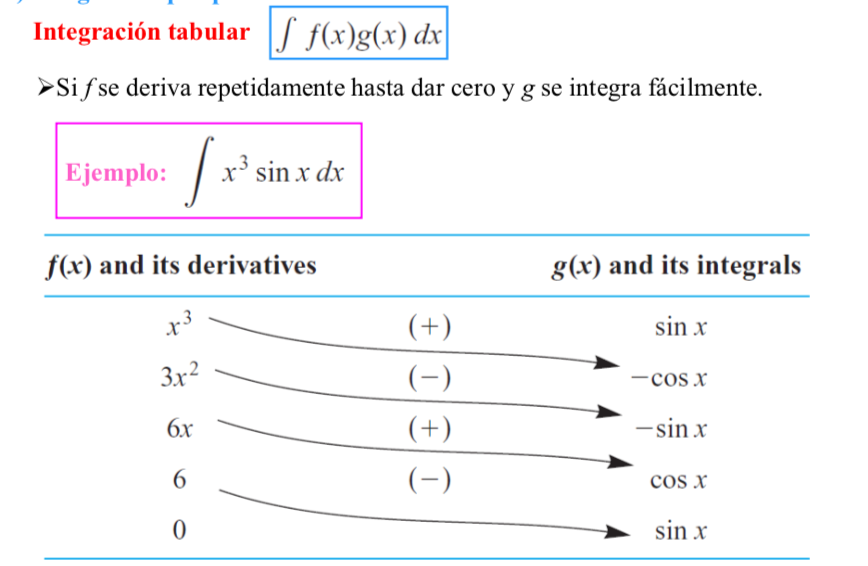
\includegraphics[width=1\textwidth]{imagenes/imagenes07/T07IM04.png}
	\end{figure}

\vspace{3mm}

\begin{ejre}
	
	Resolución ASTUTA de $\displaystyle \int 20 \tan^6 x \; \dd x = \; \to \; $
\end{ejre}

\begin{proofw}\renewcommand{\qedsymbol}{$\diamond$}	 

Efectuad la siguiente división (como si fuesen polinomios en la variable $\tan x$:

$\dfrac {\tan^6 x}{\tan^2 x + 1}= (\tan^4 x- \tan^2 x + 1) + \dfrac {-1}{\tan^2 x + 1} \to \; $  Prueba de la división ($D=d\cdot c+r$):

$\tan^6 x=  (\tan^4 x- \tan^2 x + 1)\cdot (\tan^2 x + 1) - 1\; $ Integrando:

\vspace{3mm}

\vspace{3mm}

$\to \; = \displaystyle 20 \int \left[  (\tan^4 x- \tan^2 x + 1)\cdot (\tan^2 x + 1) - 1 \right] \; \dd x =$

$=\displaystyle 20 \left[ \dfrac {\tan^5 x}{5} - \dfrac {\tan^3 x}{3} + \tan x -x  \right] + \mathcal C$
	
\end{proofw}

\begin{ejre}
	Integral resuelta de 4 formas distintas: $\displaystyle \int \sin x \; \cos x \; \dd x = \; \to $
\end{ejre}

\begin{proofw}\renewcommand{\qedsymbol}{$\diamond$}	 

Veamos los cuatro métodos:

\vspace{3mm}

$\circ \quad$ Cambio de variable: $\sin x = t \to \dd t= \cos x \dd x$	

$\to \; = \displaystyle \int t \; \dd t = \frac {t^2}{2}= \dfrac {\sin^2 x}{2} + \mathcal C$

\vspace{3mm} 
$\circ \quad$ Cambio de variable: $\cos x = t \to \dd t= -\sin x \dd x$	

$\to \; = \displaystyle - \int t\; \dd t = -\frac {t^2}{2}= -\dfrac {\cos^2 x}{2}+ \mathcal C$

\textcolor{gris}{Obviamente se trata de otra primitiva de la misma función pues la diferencia es una constante. Recuérdese el teorema fundamental del cálculo integral \ref{teor:fdmtalCI}} 

\vspace{3mm} 
$\circ \quad$ Método por partes: $u=\sin x \to \dd u = \cos x \; \dd x ; \qquad \dd v= \cos x \; \dd x \to v= \sin x $

$\to\; =\displaystyle \sin^2 x - \int \sin x \cos x \; \dd x\; $ Qué es la integral de partida, luego:

$I=\sin^2 x - I \; \to \; I=\displaystyle \int \sin x \; \cos x \; \dd x = \dfrac {\sin^2 x}{2} + \mathcal C$

\vspace{3mm} 
$\circ \quad$ Transformación en productos (apéndice \ref{Kit})

$\sin a \cdot \cos b = \frac 1 2 [\sin (a+b) + \sin(a-b)]$

$\to \; = \frac 1 2 \displaystyle \int \left( \sin 2x + \cancelto {0}{sin 0}  \right) \; \dd x= \frac 1 4 \int 2 \sin 2x \; \dd x=-\frac 1 4 \cos 2x +\mathcal C$

\textcolor{gris}{Obviamente se trata de otra primitiva de la misma función pues la diferencia es una constante (solo hay que recordar la fórmula del $\cos 2 x$). Recuérdese el teorema fundamental del cálculo integral \ref{teor:fdmtalCI}}

\end{proofw}




\begin{ejre}
	

 En los ejemplos que siguen se deducen cosas contradictorias, ?`dónde falla el razonamiento:

$\to \; I=\displaystyle \int \dfrac 1 x \, \dd x = \left[ \begin{matrix} u=\frac 1 x & \dd u = -\frac 1 {x^2} \dd v \\ \dd x & v= x = \end{matrix} \right] =1-\int x \left( - \frac 1 {x^2} \right) \dd x=1 + I \Rightarrow \boxed{\; 0=1\;} $

$\quad$


$\to \left[ \begin{matrix}
 I=\displaystyle \int (x+1)^2 \dd x =\frac {(x+1)^3}{3}=\frac 1 3 x^3 + x^2 + x + \frac 1 3  \\  
 I=\displaystyle \int (x^2+2x+1)\; \dd x= \frac 1 3 x^3 + x^2 + x  \end{matrix} \right] \Rightarrow \frac 1 3 = 0 \to  \boxed{\; 0 = 1 \;} $
\end{ejre}

 
 \begin{proofw}\renewcommand{\qedsymbol}{$\diamond$}
 
 
 \rotatebox{180}{\leftline{\textcolor{gris}{!` Falta la constante de integración en ambos casos !}}}
 

 
 \end{proofw}


\textbf{USOS DE LAS INTEGRALES.}

Una ecuación diferencial es una ecuación matemática que relaciona una función con sus derivadas. En las matemáticas aplicadas, las funciones usualmente representan cantidades físicas, las derivadas representan sus razones de cambio, y la ecuación define la relación entre ellas. Como estas relaciones son muy comunes, las ecuaciones diferenciales juegan un rol primordial en muchas disciplinas, incluyendo la ingeniería, la física, la economía, y la biología.

Veamos un \underline{ejemplo}:


Un veterinario de Valencia planea llevar un león marino a Barcelona. El animal debe viajar cubierto durante el viaje con una manta mojada. En cualquier tiempo $t$, la manta perderá humedad, debido a la evaporación, a una razón proporcional a la cantidad de agua $y(t)$ presente en la manta. Inicialmente la manta contendrá $40l$ de agua de mar y sabemos que esta cantidad se reducirá a la mitad a las dos horas del viaje. Estamos interesados en encontrar una ecuación diferencial que describa el problema y determinar si el león llegará en buen estado a su destino, para lo cual la humedad de la manta ha de ser superior a los $10l$ de agua marina.

\vspace{4mm}

$y(t)$ es la cantidad de agua en la manta en el instante $t$ ($t$ en $h$ y $y$ en $l$ de agua de mar.)

El cambio en la cantidad de agua $y(t)$, es decir, $y'(t)= \dfrac {\dd y}{\dd t}$ es proporcional a la cantidad de agua presente en la manta en ese momento:

$y'(t)=k\cdot y(t); \; $ con $k\le 0, \; y(0)=40, \; y(2)=20$ (*)

Usando `notación de Leibniz': $\dfrac {\dd y}{\dd t}=k \; y \to \dfrac {\dd y}{\dd t}= k \; \dd t\; $, integrando: (recordad la imagen \ref{mates-fisics})

$\displaystyle \int \dfrac {\dd y}{\dd t}= \int k \; \dd t \to \mathrm{ln}y= k\cdot t  \to y= e^{k\cdot t + \mathcal C}=e^{k\cdot t} \cdot e^{\mathcal C}\to  \boxed {\; y= A\cdot e^{k\cdot t}\; } $

De las condiciones del problema (*): $A=40; \; k=-0.35$

La ecuación que describe la cantidad de agua de la manta en cada momento es:  

\hspace{20mm} $\boxed {\; y= 40 e^{-0.35\; t}\; }$ 

Cuando $y=10\; h \; \to \; 10=40e^{-0.35 t} \; $. Tomando logaritmos: $ \; t = 4\; h$

En Google Maps encontramos Valencia-Barcelona, por A7, $351 \; km$ , a una media de $100\; km/h$ tardaríamos unas $3.5\; h$ aprox, con lo que el león marino llegaría en buenas condiciones.



\textbf{?`Te atreves tú?}: 

El $_{  }^{ 239 }{ Pu }$ se desintegra en $_{  }^{ 235 }{ U }$ y una partícula $\alpha$ (núcleo de Helio), según la reacción nuclear: $\;_{  }^{ 239 }{ Pu } \; \to \; _{  }^{ 235 }{U} \; + \; _{ 2 }^{ 4 } {He}\; $. Después de 15 años se determina que el $0.0043 \%$ de la cantidad inicial $A_0$ de plutonio se ha desintegrado. Determina la \emph{semivida} (tiempo en que la cantidad del isótopo radiactivo se reduce a la mitad) de este isótopo de  Plutonio si la rapidez de desintegración es proporcional a la cantidad de plutonio presente en la muestra.










